\chapter{Kế hoạch quản lý chi tiết}
\section{Kế hoạch quản lý phạm vi}
\subsection{Phạm vi công việc}
\subsubsection{Phạm vi công việc Khảo sát}
\begin{itemize}
    \item \textbf{Tên Công Việc:} Khảo sát
    \item \textbf{Mô tả công việc:}
          \begin{itemize}
              \item Trao đổi những vấn đề mà doanh nghiệp đang gặp phải trong quá trình quản lý Nhân sự - Tiền lương.
              \item Khảo sát về mong muốn, yêu cầu của doanh nghiệp đối với hệ thống.
              \item Tìm hiểu quy trình quản lý Nhân sự - Tiền lương của doanh nghiệp.
          \end{itemize}
    \item \textbf{Các Sản phẩm của công việc:}
          \begin{itemize}
              \item Báo cáo khảo sát chi tiết
              \item Tài liệu mô tả yêu cầu chức năng và phi chức năng
              \item Tài liệu mô tả quy trình nghiệp vụ
              \item Hồ sơ khảo sát hoàn chỉnh
          \end{itemize}
    \item \textbf{Yêu cầu đánh giá:}
          \begin{itemize}
              \item Báo cáo tài liệu phân tích yêu cầu khách hàng phải rõ ràng và dễ hiểu.
              \item Hoàn thành công việc trong thời gian quy định, không quá 5 ngày.
          \end{itemize}
\end{itemize}
\subsubsection{Phạm vi công việc Khảo sát}
\begin{itemize}
    \item \textbf{Tên Công Việc:} Khảo sát
    \item \textbf{Mô tả công việc:}
          \begin{itemize}
              \item Trao đổi những vấn đề mà doanh nghiệp đang gặp phải trong quá trình quản lý Nhân sự - Tiền lương.
              \item Khảo sát về mong muốn, yêu cầu của doanh nghiệp đối với hệ thống.
              \item Tìm hiểu quy trình quản lý Nhân sự - Tiền lương của doanh nghiệp.
          \end{itemize}
    \item \textbf{Các Sản phẩm của công việc:}
          \begin{itemize}
              \item Báo cáo khảo sát chi tiết
              \item Tài liệu mô tả yêu cầu chức năng và phi chức năng
              \item Tài liệu mô tả quy trình nghiệp vụ
              \item Hồ sơ khảo sát hoàn chỉnh
          \end{itemize}
    \item \textbf{Yêu cầu đánh giá:}
          \begin{itemize}
              \item Báo cáo tài liệu phân tích yêu cầu khách hàng phải rõ ràng và dễ hiểu.
              \item Hoàn thành công việc trong thời gian quy định, không quá 5 ngày.
          \end{itemize}
\end{itemize}

\subsubsection{Phạm vi công việc Phân tích và thiết kế hệ thống}
\begin{itemize}
    \item \textbf{Tên Công Việc:} Phân tích và thiết kế hệ thống
    \item \textbf{Mô tả công việc:}
          \begin{itemize}
              \item Phân tích từ yêu cầu và vấn đề khách hàng thành các yêu cầu cho hệ thống
              \item Thiết kế hệ thống dựa trên kết quả phân tích
          \end{itemize}
    \item \textbf{Các sản phẩm của công việc:}
          \begin{itemize}
              \item Báo cáo phân tích quy trình nghiệp vụ chi tiết cho các phần:
                    \begin{itemize}
                        \item Quản lý nhân sự
                        \item Quản lý phần chấm công
                        \item Quản lý hồ sơ tiền lương
                        \item Thanh toán lương
                    \end{itemize}
              \item Báo cáo phân tích yêu cầu chi tiết cho các phần:
                    \begin{itemize}
                        \item Yêu cầu giao diện
                        \item Yêu cầu chức năng
                    \end{itemize}
              \item Các biểu đồ thiết kế hệ thống bao gồm:
                    \begin{itemize}
                        \item Biểu đồ usecase
                        \item Biểu đồ lớp
                        \item Biểu đồ tuần tự
                        \item Biểu đồ hoạt động
                    \end{itemize}
              \item Thiết kế cơ sở dữ liệu chi tiết cho các phần:
                    \begin{itemize}
                        \item Nhân sự
                        \item Hồ sơ lương
                        \item Phần chấm công
                        \item Thanh toán lương
                    \end{itemize}
              \item Các thiết kế giao diện chi tiết cho các phần:
                    \begin{itemize}
                        \item Quản lý nhân sự
                        \item Quản lý hồ sơ lương
                        \item Quản lý phần chấm công
                        \item Thanh toán lương
                    \end{itemize}
              \item Báo cáo tổng hợp và lập bản báo cáo yêu cầu hệ thống
              \item Báo cáo tổng hợp và lập bản báo cáo kiến trúc hệ thống
              \item Báo cáo tổng hợp và lập bản thiết kế giao diện
              \item Hồ sơ phân tích thiết kế
          \end{itemize}
    \item \textbf{Yêu cầu đánh giá:}
    \begin{itemize}
        \item Tài liệu phân tích và thiết kế phải đúng theo tài liệu phân tích yêu cầu khách hàng
        \item Hoàn thành công việc trong thời gian quy định, không quá 15 ngày
    \end{itemize}
\end{itemize}
\subsubsection{Phạm vi công việc Xây dựng và phát triển}
\begin{itemize}
    \item \textbf{Tên Công Việc:} Xây dựng và phát triển
    \item \textbf{Mô tả công việc:}
    \begin{itemize}
        \item Lập trình các chức năng của hệ thống
        \item Tạo tài liệu thiết kế hệ thống
    \end{itemize}
    \item \textbf{Các sản phẩm của công việc:}
    \begin{itemize}
        \item Hệ thống hoàn chỉnh bao gồm các phần:
        \begin{itemize}
            \item Cơ sở dữ liệu
            \item Front-end
            \item Back-end
        \end{itemize}
        \item Báo cáo chi tiết về quá trình xây dựng và phát triển hệ thống
        \item Tài liệu hướng dẫn sử dụng và quản lý hệ thống
    \end{itemize}
    \item \textbf{Yêu cầu đánh giá:}
    \begin{itemize}
        \item Hoàn thành lập trình ứng dụng đúng với tài liệu đặc tả và thiết kế hệ thống
        \item Hoàn thành công việc trong thời gian quy định, không quá 25 ngày
    \end{itemize}
\end{itemize}

\subsubsection{Phạm vi công việc Kiểm thử}
\begin{itemize}
    \item \textbf{Tên Công Việc:} Kiểm thử
    \item \textbf{Mô tả công việc:}
    \begin{itemize}
        \item Kiểm tra và thử nghiệm hệ thống để đảm bảo tính chính xác và đáng tin cậy của hệ thống
        \item Xác định và khắc phục lỗi hoặc sai sót trong chức năng và giao diện hệ thống so với tài liệu đặc tả và yêu cầu ban đầu
    \end{itemize}
    \item \textbf{Các sản phẩm của công việc:}
    \begin{itemize}
        \item Phần mềm hoàn chỉnh sau kiểm thử bao gồm:
        \begin{itemize}
            \item Hồ sơ kiểm thử hoàn chỉnh
            \item Testcase chi tiết cho các chức năng của hệ thống
            \item Kết quả chạy testcase
            \item Báo cáo kiểm tra và sửa lỗi
            \item Báo cáo chi tiết về quá trình kiểm thử và sửa lỗi
            \item Tài liệu hướng dẫn sử dụng và quản lý phần mềm sau kiểm thử
        \end{itemize}
    \end{itemize}
    \item \textbf{Yêu cầu đánh giá:}
    \begin{itemize}
        \item Hoàn thành việc kiểm thử hệ thống, đảm bảo không còn bất kỳ sai sót nào
        \item Hoàn thành công việc trong thời gian quy định, không quá 7 ngày
    \end{itemize}
\end{itemize}
\subsubsection{Phạm vi công việc Triển khai và Bàn giao}
\begin{itemize}
    \item \textbf{Tên Công Việc:} Triển khai và bàn giao
    \item \textbf{Mô tả công việc:}
    \begin{itemize}
        \item Tiến hành cài đặt hệ thống
        \item Hướng dẫn sử dụng hệ thống
        \item Bàn giao hệ thống cho khách hàng
    \end{itemize}
    \item \textbf{Các sản phẩm của công việc:}
    \begin{itemize}
        \item Phần mềm hoàn chỉnh sau chuyển giao bao gồm:
        \begin{itemize}
            \item Hồ sơ triển khai và chuyển giao hoàn chỉnh
            \item Tài liệu hướng dẫn sử dụng
            \item Báo cáo chi tiết về quá trình bàn giao và cài đặt
            \item Báo cáo chi tiết về quá trình đào tạo và sử dụng
        \end{itemize}
        \item Báo cáo chi tiết về quá trình chuyển giao
        \item Tài liệu hướng dẫn sử dụng và quản lý hệ thống sau khi chuyển giao
    \end{itemize}
    \item \textbf{Yêu cầu đánh giá:}
    \begin{itemize}
        \item Hoàn thành việc cài đặt hệ thống và hướng dẫn sử dụng thành công
        \item Bàn giao hệ thống đúng với yêu cầu của khách hàng
        \item Hoàn thành công việc trong thời gian quy định, không quá 8 ngày
    \end{itemize}
\end{itemize}
\subsection{Sơ đồ phân rã công việc}
\begin{figure}[H]
    \centering
    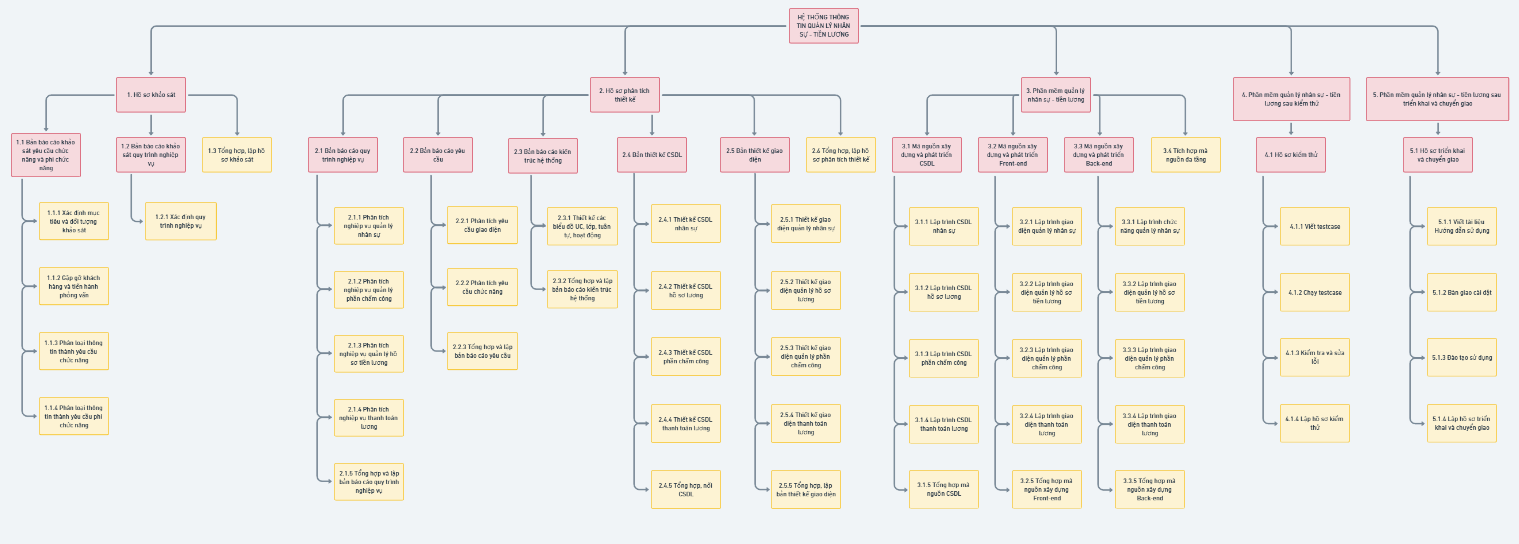
\includegraphics[width=\textwidth]{images/sodophanratongquat.png}
    \caption{Sơ đồ phân rã công việc}
\end{figure}
\begin{figure}[H]
    \centering
    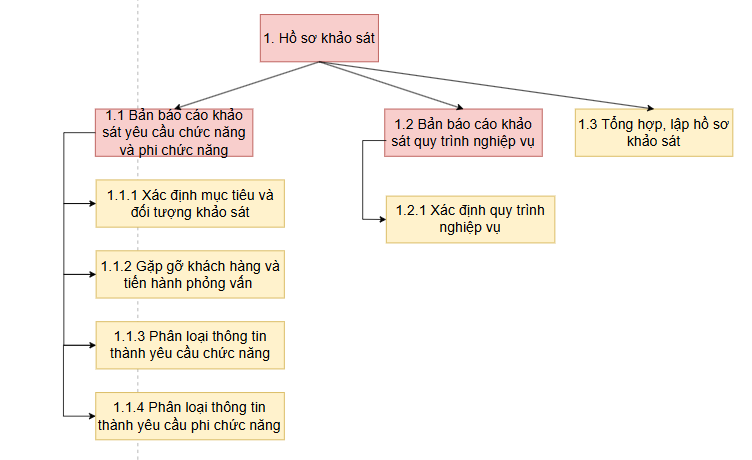
\includegraphics[width=\textwidth]{images/hskhaosat.png}
    \caption{Phân rã chi tiết Hồ sơ khảo sát}
\end{figure}
\begin{figure}[H]
    \centering
    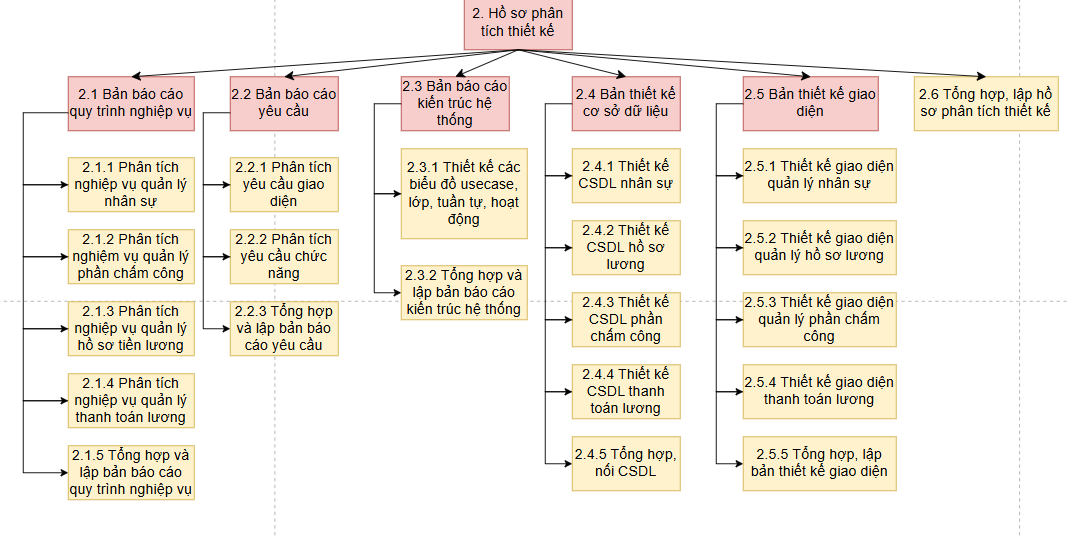
\includegraphics[width=\textwidth]{images/hspttk.png}
    \caption{Phân rã chi tiết hồ sơ phân tích thiết kế}
\end{figure}
\begin{figure}[H]
    \centering
    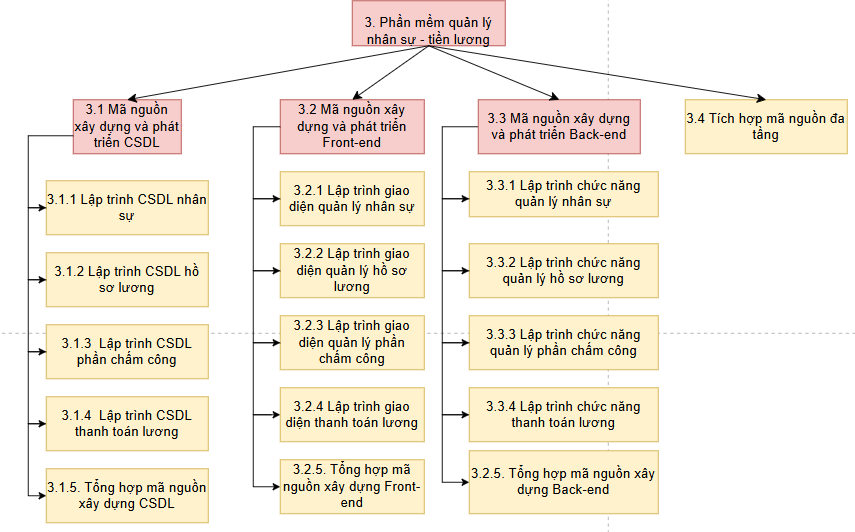
\includegraphics[width=\textwidth]{images/pmquanlyns-tl.png}
    \caption{Phân rã chi tiết phần mềm quản lý nhân sự - tiền lương}
\end{figure}
\begin{figure}[H]
    \centering
    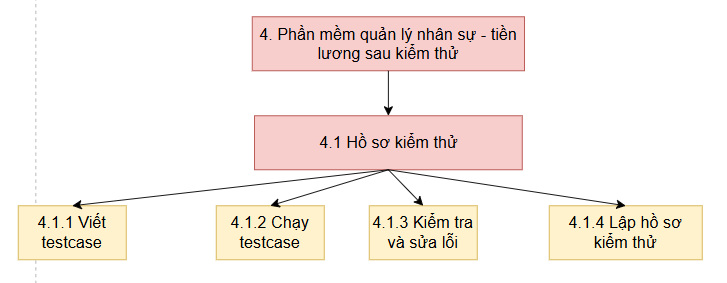
\includegraphics[width=\textwidth]{images/pmsaukiemthu.png}
    \caption{Phân rã chi tiết phần mềm quản lý nhân sự - tiền lương sau kiểm thử}
\end{figure}
\begin{figure}[H]
    \centering
    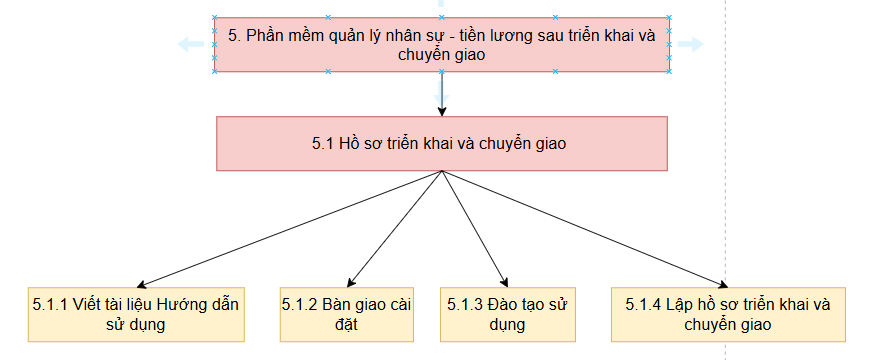
\includegraphics[width=\textwidth]{images/pmsautrienkhai.png}
    \caption{Phân rã chi tiết phần mềm quản lý nhân sự - tiền lương sau triển khai và chuyển giao}
\end{figure}
\subsection{Biên bản phạm vi công việc}
% Xác định mục tiêu và đối tượng khảo sát
\subsubsection{Xác định mục tiêu và đối tượng khảo sát}
\fbox{
    \begin{minipage}{\textwidth}
    \begin{center}
    \textbf{\huge BIÊN BẢN PHẠM VI CÔNG VIỆC}
    \end{center}
    \vspace{0.5cm}
    \noindent \textbf{Tên công việc:} Xác định mục tiêu và đối tượng khảo sát \\
    \textbf{Ngày bắt đầu:} 24/11/2024 \\
    \textbf{Ngày kết thúc:} 24/11/2024 \\
    \textbf{Người quản lý:} Hoàng Thu Phương \\
    \noindent\rule{\textwidth}{0.4pt}  % Đoạn này tạo đường kẻ ngang
    \noindent \textbf{Sản phẩm công việc:}
    \begin{itemize}
        \item Báo cáo xác định mục tiêu khảo sát chi tiết.
        \item Danh sách đối tượng khảo sát được phân loại.
        \item Tài liệu hướng dẫn thực hiện khảo sát dựa trên mục tiêu và đối tượng đã xác định.
    \end{itemize}
    \noindent \textbf{Tiêu chí của sản phẩm:}
    \begin{itemize}
        \item Báo cáo phải chi tiết, rõ ràng và chính xác về mục tiêu khảo sát.
        \item Danh sách đối tượng khảo sát phải đầy đủ và phân loại rõ ràng.
        \item Tài liệu hướng dẫn phải dễ hiểu và có thể áp dụng cho các bước tiếp theo của quá trình khảo sát.
    \end{itemize}
    \noindent \textbf{Mô tả công việc:}
    \begin{itemize}
        \item Thu thập thông tin từ các bên liên quan để xác định mục tiêu cụ thể.
        \item Lập danh sách đối tượng cần khảo sát.
        \item Đưa ra các phương pháp khảo sát phù hợp (ví dụ: khảo sát trực tuyến, phỏng vấn, bảng hỏi,...).
    \end{itemize}
    \noindent \textbf{Thời gian thực hiện:} 1 ngày \\
    \noindent \textbf{Nguồn lực:}
    \begin{itemize}
        \item \textbf{Công cụ:} Phần mềm khảo sát, bảng hỏi mẫu.
        \item \textbf{Nhân lực:} Nhân viên hỗ trợ khảo sát và phân tích dữ liệu.
        \item \textbf{Dữ liệu:} Thông tin cơ bản từ khách hàng, người dùng, đối tượng mục tiêu.
    \end{itemize}
\end{minipage}
}
\newpage %sang trang mới
\fbox{
    \begin{minipage}{\textwidth}
        \noindent \textbf{Ràng buộc:}
        \begin{itemize}
            \item Thời gian hoàn thành chỉ trong 1 ngày.
            \item Số lượng đối tượng khảo sát phù hợp với quy mô dự án.
            \item Đảm bảo độ chính xác và tính khả thi của kế hoạch khảo sát.
        \end{itemize}
        \noindent \textbf{Nhân sự:}
        \begin{longtable}{|c|c|}
        \hline
        \textbf{Người thực hiện} & \textbf{Vai trò} \\
        \hline
        Nguyễn Ngọc Quang & Xác định mục tiêu, đối tượng khảo sát \\
        \hline
        \end{longtable}
        \noindent \textbf{Chi phí người thực hiện:} 600.000 VNĐ
        \vspace{1cm}
        \begin{flushleft}
            \hspace{8cm} \textbf{NGƯỜI THỰC HIỆN} \\
            \hspace{8.8cm} (Ký tên, họ tên) \\
            \vspace{1cm}
        \end{flushleft}
    \end{minipage}
}
% Gặp gỡ khách hàng và tiến hành phỏng vấn
\subsubsection{Gặp gỡ khách hàng và tiến hành phỏng vấn}
\fbox{
    \begin{minipage}{\textwidth}
    \begin{center}
    \textbf{\huge BIÊN BẢN PHẠM VI CÔNG VIỆC}
    \end{center}
    \vspace{0.5cm}
    \noindent \textbf{Tên công việc:} Gặp gỡ khách hàng và tiến hành phỏng vấn \\
    \textbf{Ngày bắt đầu:} 25/11/2024 \\
    \textbf{Ngày kết thúc:} 25/11/2024 \\
    \textbf{Người quản lý:} Hoàng Thu Phương \\
    \noindent\rule{\textwidth}{0.4pt}  % Đoạn này tạo đường kẻ ngang
    \noindent \textbf{Sản phẩm công việc:}
    \begin{itemize}
        \item Báo cáo chi tiết về cuộc gặp gỡ và phỏng vấn khách hàng.
        \item Bản ghi chép các câu hỏi và câu trả lời từ khách hàng.
        \item Tài liệu tổng hợp các yêu cầu và mong muốn của khách hàng.
    \end{itemize}
    \noindent \textbf{Tiêu chí của sản phẩm:}
    \begin{itemize}
        \item Báo cáo phải chi tiết, rõ ràng và chính xác về nội dung cuộc gặp gỡ và phỏng vấn.
        \item Bản ghi chép phải đầy đủ và chính xác các câu hỏi và câu trả lời.
        \item Tài liệu tổng hợp phải dễ hiểu và có thể áp dụng cho các bước tiếp theo của dự án.
    \end{itemize}
    \end{minipage}
}
\newpage % Sang trang mới
\fbox{
    \begin{minipage}{\textwidth}
        \noindent \textbf{Mô tả công việc:}
        \begin{itemize}
            \item Lên lịch và sắp xếp cuộc gặp gỡ với khách hàng.
            \item Chuẩn bị các câu hỏi phỏng vấn liên quan đến dự án.
            \item Tiến hành phỏng vấn khách hàng để thu thập thông tin và yêu cầu.
            \item Ghi chép lại các câu hỏi và câu trả lời từ khách hàng.
            \item Tổng hợp và phân tích thông tin thu thập được từ cuộc phỏng vấn.
        \end{itemize}
        \noindent \textbf{Thời gian thực hiện:} 1 ngày \\
        \noindent \textbf{Nguồn lực:}
        \begin{itemize}
            \item \textbf{Thiết bị:} Máy tính xách tay, thiết bị ghi âm, công cụ ghi chú.
            \item \textbf{Tài liệu:} Danh sách câu hỏi phỏng vấn và các biểu mẫu cần thiết.
            \item \textbf{Nhân sự:} Người điều phối buổi phỏng vấn và người ghi nhận thông tin.
        \end{itemize}
        \noindent \textbf{Ràng buộc:}
        \begin{itemize}
            \item Đảm bảo thông tin thu thập được chính xác và đầy đủ.
            \item Thời gian hoàn thành trong 1 ngày.
            \item Đảm bảo tính chính xác và đầy đủ của thông tin thu thập được.
            \item Tuân thủ các nguyên tắc bảo mật và quyền riêng tư của khách hàng.
        \end{itemize}
        \noindent \textbf{Nhân sự:}
        \begin{longtable}{|c|c|}
        \hline
        \textbf{Người thực hiện} & \textbf{Vai trò} \\
        \hline
        Hoàng Đức Phong & Phỏng vấn, ghi nhận thông tin \\
        \hline
        \end{longtable}
        \noindent \textbf{Chi phí người thực hiện:} 600.000 VNĐ
        \vspace{1cm}
        \begin{flushleft}
            \hspace{8cm} \textbf{NGƯỜI THỰC HIỆN} \\
            \hspace{8.8cm} (Ký tên, họ tên) \\
            \vspace{1cm}
        \end{flushleft}
    \end{minipage}
}
% Phân loại thông tin thành yêu cầu chức năng
\subsubsection{Phân loại thông tin thành yêu cầu chức năng}
\fbox{
    \begin{minipage}{\textwidth}
    \begin{center}
    \textbf{\huge BIÊN BẢN PHẠM VI CÔNG VIỆC}
    \end{center}
    \vspace{0.5cm}
    \noindent \textbf{Tên công việc:} Phân loại thông tin thành yêu cầu chức năng \\
    \textbf{Ngày bắt đầu:} 26/11/2024 \\
    \textbf{Ngày kết thúc:} 26/11/2024 \\
    \textbf{Người quản lý:} Hoàng Thu Phương \\
    \noindent\rule{\textwidth}{0.4pt}  % Đoạn này tạo đường kẻ ngang
    \noindent \textbf{Sản phẩm công việc:}
    \begin{itemize}
        \item Danh sách yêu cầu chức năng được phân loại theo từng nhóm cụ thể.
        \item Báo cáo chi tiết về các yêu cầu chức năng và tài liệu mô tả đầy đủ.
    \end{itemize}
    \noindent \textbf{Tiêu chí của sản phẩm:}
    \begin{itemize}
        \item Danh sách yêu cầu chức năng phải đầy đủ, chi tiết và phân loại rõ ràng.
        \item Báo cáo phải rõ ràng, chính xác và dễ hiểu.
        \item Tài liệu hướng dẫn phải dễ hiểu và có thể áp dụng cho các bước tiếp theo của quá trình phát triển phần mềm.
    \end{itemize}
    \noindent \textbf{Mô tả công việc:}
    \begin{itemize}
        \item Xem xét và đánh giá lại thông tin đã thu thập từ khách hàng.
        \item Phân tích từng thông tin để xác định các yêu cầu chức năng phù hợp.
        \item Phân loại các yêu cầu chức năng thành nhóm (ví dụ: quản lý người dùng, quản lý dữ liệu, báo cáo,...).
        \item Xây dựng tài liệu chi tiết bao gồm các yêu cầu chức năng được xác định.
    \end{itemize}
    \noindent \textbf{Thời gian thực hiện:} 1 ngày \\
    \noindent \textbf{Nguồn lực:}
    \begin{itemize}
        \item \textbf{Tài liệu:} Thông tin đã thu thập từ buổi phỏng vấn và tài liệu liên quan.
        \item \textbf{Công cụ:} Phần mềm xử lý văn bản, bảng tính (Excel), công cụ quản lý yêu cầu (ví dụ: Trello, Jira,...).
        \item \textbf{Nhân sự:} Nhân viên phân tích yêu cầu và tổng hợp dữ liệu.
    \end{itemize}
    \end{minipage}
}
\newpage % Sang trang mới
\fbox{
    \begin{minipage}{\textwidth}
    \noindent \textbf{Ràng buộc:}
    \begin{itemize}
        \item Thời gian hoàn thành trong 1 ngày.
        \item Đảm bảo tính chính xác và đầy đủ của các yêu cầu chức năng.
        \item Các yêu cầu chức năng cần được mô tả rõ ràng, dễ hiểu và có tính khả thi.
    \end{itemize}
        \noindent \textbf{Nhân sự:}
        \begin{longtable}{|c|c|}
        \hline
        \textbf{Người thực hiện} & \textbf{Vai trò} \\
        \hline
        Hoàng Thu Phương & Người thực hiện phân tích \\
        \hline
        \end{longtable}
        \noindent \textbf{Chi phí người thực hiện:} 1.000.000 VNĐ
        \vspace{1cm}
        \begin{flushleft}
            \hspace{8cm} \textbf{NGƯỜI THỰC HIỆN} \\
            \hspace{8.8cm} (Ký tên, họ tên) \\
            \vspace{1cm}
        \end{flushleft}
    \end{minipage}
}
% Điều chỉnh căn khoảng cách sau
% Phân loại thông tin thành yêu cầu phi chức năng
\subsubsection{Phân loại thông tin thành yêu cầu phi chức năng}
\fbox{
    \begin{minipage}{\textwidth}
    \begin{center}
    \textbf{\huge BIÊN BẢN PHẠM VI CÔNG VIỆC}
    \end{center}
    \vspace{0.5cm}
    \noindent \textbf{Tên công việc:} Phân loại thông tin thành yêu cầu phi chức năng \\
    \textbf{Ngày bắt đầu:} 26/11/2024 \\
    \textbf{Ngày kết thúc:} 26/11/2024 \\
    \textbf{Người quản lý:} Hoàng Thu Phương \\
    \noindent\rule{\textwidth}{0.4pt}  % Đoạn này tạo đường kẻ ngang
    \noindent \textbf{Sản phẩm công việc:}
    \begin{itemize}
        \item Danh sách yêu cầu phi chức năng chi tiết và phân loại rõ ràng.
        \item Báo cáo mô tả các yêu cầu phi chức năng của hệ thống.
        \item Tài liệu làm cơ sở cho quá trình thiết kế, phát triển và kiểm thử phần mềm.
    \end{itemize}
    \noindent \textbf{Tiêu chí của sản phẩm:}
    \begin{itemize}
        \item Danh sách yêu cầu phi chức năng phải đầy đủ, chi tiết và phân loại rõ ràng.
        \item Báo cáo phải rõ ràng, chính xác và dễ hiểu.
        \item Tài liệu hướng dẫn phải dễ hiểu và có thể áp dụng cho các bước tiếp theo của quá trình phát triển phần mềm.
    \end{itemize}
    \noindent \textbf{Mô tả công việc:}
    \begin{itemize}
        \item Xem xét và đánh giá thông tin đã thu thập từ khách hàng.
        \item Phân tích thông tin để xác định các yêu cầu phi chức năng.
        \item Phân loại các yêu cầu phi chức năng theo từng nhóm cụ thể.
        \item Lập danh sách yêu cầu phi chức năng chi tiết.
        \item Xây dựng báo cáo mô tả các yêu cầu phi chức năng của hệ thống.
        \item Tạo tài liệu hướng dẫn sử dụng yêu cầu phi chức năng cho quá trình phát triển phần mềm.
    \end{itemize}
    \vspace{0.5cm}
    \noindent \textbf{Thời gian thực hiện:} 1 ngày \\
    \noindent \textbf{Nguồn lực:}
    \begin{itemize}
        \item \textbf{Tài liệu:} Thông tin từ các cuộc họp, phỏng vấn khách hàng.
        \item \textbf{Công cụ:} Phần mềm xử lý văn bản, bảng tính (Excel), công cụ quản lý yêu cầu.
        \item \textbf{Nhân sự:} Nhân viên phân tích yêu cầu và lập danh sách yêu cầu phi chức năng.
    \end{itemize}
    \vspace{0.5cm}
    \noindent \textbf{Ràng buộc:}
    \begin{itemize}
        \item Thời gian hoàn thành trong 1 ngày.
        \item Đảm bảo tính chính xác và đầy đủ của các yêu cầu phi chức năng.
        \item Thông tin thu thập và phân tích phải đầy đủ để đáp ứng tiêu chuẩn phát triển phần mềm.
    \end{itemize}
    \end{minipage}
}
\newpage % Sang trang mới
\fbox{
    \begin{minipage}{\textwidth}
        \noindent \textbf{Nhân sự:}
        \begin{longtable}{|c|c|}
        \hline
        \textbf{Người thực hiện} & \textbf{Vai trò} \\
        \hline
        Đỗ Tiến Phát & Người thực hiện phân tích \\
        \hline
        \end{longtable}
        \vspace{0.5cm}
        \noindent \textbf{Chi phí người thực hiện:} 600.000 VNĐ
        \vspace{1cm}
        \begin{flushleft}
            \hspace{8cm} \textbf{NGƯỜI THỰC HIỆN} \\
            \hspace{8.8cm} (Ký tên, họ tên) \\
            \vspace{1cm}
        \end{flushleft}
    \end{minipage}
}
% 
\subsubsection{Báo cáo khảo sát yêu cầu chức năng và phi chức năng}
\fbox{
    \begin{minipage}{\textwidth}
    \begin{center}
    \textbf{\huge BIÊN BẢN PHẠM VI CÔNG VIỆC}
    \end{center}
    \vspace{0.5cm}
    \noindent \textbf{Tên công việc:} Báo cáo khảo sát yêu cầu chức năng và phi chức năng \\
    \textbf{Ngày bắt đầu:} 24/11/2024 \\
    \textbf{Ngày kết thúc:} 26/11/2024 \\
    \textbf{Người quản lý:} Hoàng Thu Phương \\
    \noindent\rule{\textwidth}{0.4pt}  % Đoạn này tạo đường kẻ ngang
    \noindent \textbf{Sản phẩm công việc:}
    \begin{itemize}
        \item Bản báo cáo tổng hợp yêu cầu chức năng và phi chức năng của phần mềm.
        \item Phân loại chi tiết các yêu cầu chức năng theo nhóm cụ thể.
        \item Phân loại các yêu cầu phi chức năng theo tiêu chuẩn về hiệu suất, bảo mật, khả năng mở rộng,...
        \item Tài liệu hoàn chỉnh làm cơ sở cho giai đoạn thiết kế và phát triển phần mềm.
    \end{itemize}
    \noindent \textbf{Tiêu chí của sản phẩm:}
    \begin{itemize}
        \item Báo cáo phải chi tiết, rõ ràng và chính xác về các yêu cầu chức năng và phi chức năng.
        \item Tài liệu tổng hợp phải đầy đủ, dễ hiểu và có thể áp dụng cho các bước tiếp theo của quá trình phát triển phần mềm.
    \end{itemize}
    \noindent \textbf{Mô tả công việc:}
    \begin{itemize}
        \item Tổng hợp kết quả từ các công việc phân loại yêu cầu chức năng và phi chức năng.
        \item Đánh giá, kiểm tra lại các yêu cầu để đảm bảo tính chính xác và đầy đủ.
        \item Xây dựng bản báo cáo mô tả chi tiết:
        \begin{itemize}
            \item Yêu cầu chức năng: Các chức năng cụ thể phần mềm cần thực hiện.
            \item Yêu cầu phi chức năng: Các tiêu chí kỹ thuật như hiệu suất, bảo mật, khả năng bảo trì,...
        \end{itemize}
        \item Phối hợp với các bên liên quan để xác minh tính khả thi của các yêu cầu.
    \end{itemize}
    \vspace{0.5cm}
    \noindent \textbf{Thời gian thực hiện:} 3 ngày \\
    \noindent \textbf{Nguồn lực:}
    \begin{itemize}
        \item \textbf{Tài liệu:} Thông tin từ các buổi phỏng vấn, dữ liệu phân tích trước đó.
        \item \textbf{Công cụ:} Phần mềm xử lý văn bản, bảng tính (Excel), công cụ lập báo cáo.
        \item \textbf{Nhân sự:} Nhân viên phân tích yêu cầu và người lập báo cáo.
    \end{itemize}
    \vspace{0.5cm}
    \noindent \textbf{Ràng buộc:}
    \begin{itemize}
        \item Thời gian hoàn thành trong 3 ngày.
        \item Đảm bảo tính chính xác và đầy đủ của các yêu cầu chức năng và phi chức năng.
        \item Đảm bảo các báo cáo và tài liệu tổng hợp được lập chi tiết, rõ ràng và dễ hiểu.
    \end{itemize}
    \end{minipage}
}

\newpage % Sang trang mới

\fbox{
    \begin{minipage}{\textwidth}
        \noindent \textbf{Nhân sự:}
        \begin{longtable}{|c|c|}
        \hline
        \textbf{Người thực hiện} & \textbf{Vai trò} \\
        \hline
        Quang,Phong,Phương,Phát & Người thực hiện khảo sát \\
        \hline
        \end{longtable}
        \vspace{0.5cm}
        \noindent \textbf{Chi phí:} 5.800.000 VNĐ bao gồm:
        \begin{itemize}
            \item \textbf{Chi phí người quản lý:} 3.000.000 VNĐ
            \item \textbf{Chi phí người thực hiện:} 600.000 VNĐ x 3 = 2.800.000 VNĐ
        \end{itemize}
        \vspace{1cm}
        \begin{flushleft}
            \hspace{8cm} \textbf{NGƯỜI THỰC HIỆN} \\
            \hspace{8.8cm} (Ký tên, họ tên) \\
            \vspace{1cm}
        \end{flushleft}
    \end{minipage}
}
% 
\subsubsection{Xác định quy trình nghiệp vụ}
\fbox{
    \begin{minipage}{\textwidth}
    \begin{center}
    \textbf{\huge BIÊN BẢN PHẠM VI CÔNG VIỆC}
    \end{center}
    \vspace{0.5cm}
    \noindent \textbf{Tên công việc:} Xác định quy trình nghiệp vụ \\
    \textbf{Ngày bắt đầu:} 27/11/2024 \\
    \textbf{Ngày kết thúc:} 27/11/2024 \\
    \textbf{Người quản lý:} Hoàng Thu Phương \\
    \noindent\rule{\textwidth}{0.4pt}  % Đoạn này tạo đường kẻ ngang
    \noindent \textbf{Sản phẩm công việc:}
    \begin{itemize}
        \item Tài liệu mô tả quy trình nghiệp vụ chi tiết.
        \item Báo cáo chi tiết về quá trình xác định quy trình nghiệp vụ.
        \item Tài liệu hướng dẫn sử dụng và quản lý quy trình nghiệp vụ.
    \end{itemize}
    \noindent \textbf{Tiêu chí của sản phẩm:}
    \begin{itemize}
        \item Tài liệu mô tả quy trình nghiệp vụ phải đầy đủ, chi tiết và bao phủ tất cả các bước cần thiết.
        \item Báo cáo phải chi tiết, rõ ràng và chính xác về quá trình xác định quy trình nghiệp vụ.
        \item Tài liệu hướng dẫn phải dễ hiểu và có thể áp dụng cho các bước tiếp theo của quá trình quản lý và sử dụng quy trình nghiệp vụ.
    \end{itemize}
    \noindent \textbf{Mô tả công việc:}
    \begin{itemize}
        \item Phân tích các yêu cầu về quy trình nghiệp vụ.
        \item Thiết kế các bước quy trình nghiệp vụ chi tiết.
        \item Lập tài liệu mô tả quy trình nghiệp vụ theo thiết kế đã đề ra.
        \item Kiểm tra và xác nhận tài liệu mô tả quy trình nghiệp vụ để đảm bảo không có lỗi.
        \item Lập báo cáo chi tiết về quá trình xác định quy trình nghiệp vụ.
        \item Tạo tài liệu hướng dẫn sử dụng và quản lý quy trình nghiệp vụ.
    \end{itemize}
    \vspace{0.5cm}
    \noindent \textbf{Thời gian thực hiện:} 1 ngày \\
    \noindent \textbf{Nguồn lực:}
    \begin{itemize}
        \item \textbf{Công cụ:} Phần mềm xử lý văn bản (như Microsoft Word, Google Docs), phần mềm thiết kế quy trình (như Lucidchart).
        \item \textbf{Nhân lực:} Chuyên gia phân tích nghiệp vụ, người lập báo cáo.
        \item \textbf{Dữ liệu:} Thông tin từ các cuộc họp, phỏng vấn và tài liệu liên quan đến quy trình nghiệp vụ.
    \end{itemize}
    \vspace{0.5cm}
    \noindent \textbf{Ràng buộc:}
    \begin{itemize}
        \item Thời gian hoàn thành trong 1 ngày.
        \item Đảm bảo tính chính xác và đầy đủ của tài liệu mô tả quy trình nghiệp vụ.
        \item Đảm bảo báo cáo và tài liệu hướng dẫn được lập chi tiết, rõ ràng và dễ hiểu.
    \end{itemize}
    \end{minipage}
}

\newpage % Sang trang mới

\fbox{
    \begin{minipage}{\textwidth}
        \noindent \textbf{Nhân sự:}
        \begin{longtable}{|c|c|}
        \hline
        \textbf{Người thực hiện} & \textbf{Vai trò} \\
        \hline
        Hoàng Thu Phương & Người thực hiện phân tích \\
        \hline
        \end{longtable}
        \vspace{0.5cm}
        \noindent \textbf{Chi phí người thực hiện:} 1.000.000 VNĐ
        \vspace{1cm}
        \begin{flushleft}
            \hspace{8cm} \textbf{NGƯỜI THỰC HIỆN} \\
            \hspace{8.8cm} (Ký tên, họ tên) \\
            \vspace{1cm}
        \end{flushleft}
    \end{minipage}
}
% 
\subsubsection{Báo cáo khảo sát quy trình nghiệp vụ}
\fbox{
    \begin{minipage}{\textwidth}
    \begin{center}
    \textbf{\huge BIÊN BẢN PHẠM VI CÔNG VIỆC}
    \end{center}
    \vspace{0.5cm}
    \noindent \textbf{Tên công việc:} Báo cáo khảo sát quy trình nghiệp vụ \\
    \textbf{Ngày bắt đầu:} 27/11/2024 \\
    \textbf{Ngày kết thúc:} 27/11/2024 \\
    \textbf{Người quản lý:} Hoàng Thu Phương \\
    \noindent\rule{\textwidth}{0.4pt}  % Đoạn này tạo đường kẻ ngang
    \noindent \textbf{Sản phẩm công việc:}
    \begin{itemize}
        \item Báo cáo khảo sát quy trình nghiệp vụ chi tiết.
        \item Tài liệu mô tả quy trình nghiệp vụ hiện tại.
        \item Tài liệu đề xuất cải tiến quy trình nghiệp vụ (nếu có).
        \item Tài liệu mô tả quy trình nghiệp vụ chi tiết (sản phẩm của công việc xác định quy trình nghiệp vụ).
    \end{itemize}
    \noindent \textbf{Tiêu chí của sản phẩm:}
    \begin{itemize}
        \item Báo cáo phải chi tiết, rõ ràng và chính xác về quy trình nghiệp vụ hiện tại.
        \item Tài liệu mô tả quy trình nghiệp vụ phải đầy đủ, chi tiết và bao phủ tất cả các bước cần thiết.
        \item Tài liệu đề xuất cải tiến phải dễ hiểu và có thể áp dụng cho các bước tiếp theo của quá trình quản lý và sử dụng quy trình nghiệp vụ.
    \end{itemize}
    \noindent \textbf{Mô tả công việc:}
    \begin{itemize}
        \item Lập báo cáo chi tiết về quy trình nghiệp vụ hiện tại bao gồm các điểm mạnh, điểm yếu và đề xuất cải tiến (nếu có).
        \item Kiểm tra và xác nhận báo cáo khảo sát và tài liệu mô tả quy trình nghiệp vụ để đảm bảo không có lỗi.
        \item Tạo tài liệu hướng dẫn sử dụng và quản lý quy trình nghiệp vụ hiện tại và đề xuất cải tiến (nếu có).
    \end{itemize}
    \vspace{0.5cm}
    \noindent \textbf{Thời gian thực hiện:} 1 ngày \\
    \noindent \textbf{Nguồn lực:}
    \begin{itemize}
        \item \textbf{Công cụ:} Phần mềm xử lý văn bản (như Microsoft Word, Google Docs), phần mềm thiết kế quy trình (như Lucidchart).
        \item \textbf{Nhân lực:} Chuyên gia phân tích nghiệp vụ, người lập báo cáo.
        \item \textbf{Dữ liệu:} Thông tin từ các cuộc họp, phỏng vấn và tài liệu liên quan đến quy trình nghiệp vụ.
    \end{itemize}
    \vspace{0.5cm}
    \noindent \textbf{Ràng buộc:}
    \begin{itemize}
        \item Thời gian hoàn thành trong 1 ngày.
        \item Đảm bảo tính chính xác và đầy đủ của báo cáo khảo sát quy trình nghiệp vụ.
        \item Đảm bảo báo cáo và tài liệu hướng dẫn được lập chi tiết, rõ ràng và dễ hiểu.
    \end{itemize}
    \end{minipage}
}

\newpage % Sang trang mới

\fbox{
    \begin{minipage}{\textwidth}
        \noindent \textbf{Nhân sự:}
        \begin{longtable}{|c|c|}
        \hline
        \textbf{Người thực hiện} & \textbf{Vai trò} \\
        \hline
        Hoàng Thu Phương & Người thực hiện khảo sát quy trình nghiệp vụ \\
        \hline
        \end{longtable}
        \vspace{0.5cm}
        \noindent \textbf{Chi phí:} 2.000.000 VNĐ
        \begin{itemize}
            \item Chi phí người quản lý: 1.000.000 VNĐ
            \item Chi phí người thực hiện: 1.000.000 VNĐ
        \end{itemize}
        \vspace{1cm}
        \begin{flushleft}
            \hspace{8cm} \textbf{NGƯỜI THỰC HIỆN} \\
            \hspace{8.8cm} (Ký tên, họ tên) \\
            \vspace{1cm}
        \end{flushleft}
    \end{minipage}
}
% 
\subsubsection{Tổng hợp, lập hồ sơ khảo sát}
\fbox{
    \begin{minipage}{\textwidth}
    \begin{center}
    \textbf{\huge BIÊN BẢN PHẠM VI CÔNG VIỆC}
    \end{center}
    \vspace{0.5cm}
    \noindent \textbf{Tên công việc:} Tổng hợp, lập hồ sơ khảo sát \\
    \textbf{Ngày bắt đầu:} 28/11/2024 \\
    \textbf{Ngày kết thúc:} 28/11/2024 \\
    \textbf{Người quản lý:} Hoàng Thu Phương \\
    \noindent\rule{\textwidth}{0.4pt}  % Đoạn này tạo đường kẻ ngang
    \noindent \textbf{Sản phẩm công việc:}
    \begin{itemize}
        \item Hồ sơ khảo sát hoàn chỉnh bao gồm các thông tin chi tiết về đối tượng khảo sát, phương pháp khảo sát và kết quả khảo sát.
        \item Báo cáo phân tích kết quả khảo sát với các biểu đồ và số liệu minh họa.
        \item Tài liệu hướng dẫn sử dụng kết quả khảo sát cho các mục đích nghiên cứu và phát triển.
    \end{itemize}
    \noindent \textbf{Tiêu chí của sản phẩm:}
    \begin{itemize}
        \item Hồ sơ khảo sát phải chi tiết, rõ ràng và chính xác.
        \item Báo cáo phân tích phải có các biểu đồ và số liệu minh họa cụ thể.
        \item Tài liệu hướng dẫn phải dễ hiểu và có thể áp dụng cho các mục đích nghiên cứu và phát triển.
    \end{itemize}
    \noindent \textbf{Mô tả công việc:}
    \begin{itemize}
        \item Thu thập thông tin từ các cuộc khảo sát đã thực hiện.
        \item Tổng hợp và phân loại dữ liệu khảo sát.
        \item Phân tích dữ liệu để rút ra các kết luận chính.
        \item Lập hồ sơ khảo sát chi tiết bao gồm:
        \begin{itemize}
            \item Mục tiêu khảo sát.
            \item Đối tượng khảo sát.
            \item Phương pháp khảo sát.
            \item Kết quả khảo sát.
            \item Phân tích và kết luận.
        \end{itemize}
        \item Xây dựng báo cáo và tài liệu hướng dẫn sử dụng kết quả khảo sát.
    \end{itemize}
    \vspace{0.5cm}
    \noindent \textbf{Thời gian thực hiện:} 1 ngày \\
    \noindent \textbf{Nguồn lực:}
    \begin{itemize}
        \item \textbf{Tài liệu:} Thông tin từ các cuộc khảo sát, phỏng vấn đối tượng khảo sát.
        \item \textbf{Công cụ:} Phần mềm xử lý văn bản, bảng tính (Excel), phần mềm phân tích dữ liệu.
        \item \textbf{Nhân sự:} Nhóm phân tích dữ liệu, người lập hồ sơ khảo sát, người hỗ trợ tổng hợp dữ liệu.
    \end{itemize}
    \vspace{0.5cm}
    \noindent \textbf{Ràng buộc:}
    \begin{itemize}
        \item Thời gian hoàn thành trong 1 ngày.
        \item Đảm bảo hồ sơ khảo sát được lập chi tiết, rõ ràng và chính xác.
        \item Thông tin thu thập và phân tích phải đầy đủ để đáp ứng tiêu chuẩn nghiên cứu và phát triển.
    \end{itemize}
    \end{minipage}
}

\newpage % Sang trang mới

\fbox{
    \begin{minipage}{\textwidth}
        \noindent \textbf{Nhân sự:}
        \begin{longtable}{|c|c|}
        \hline
        \textbf{Người thực hiện} & \textbf{Vai trò} \\
        \hline
        Hoàng Đức Phong & Người tổng hợp và lập hồ sơ \\
        \hline
        \end{longtable}
        \vspace{0.5cm}
        \noindent \textbf{Chi phí:} 1.600.000 VNĐ
        \begin{itemize}
            \item Chi phí người quản lý: 1.000.000 VNĐ
            \item Chi phí người thực hiện: 600.000 VNĐ
        \end{itemize}
        \vspace{1cm}
        \begin{flushleft}
            \hspace{8cm} \textbf{NGƯỜI THỰC HIỆN} \\
            \hspace{8.8cm} (Ký tên, họ tên) \\
            \vspace{1cm}
        \end{flushleft}
    \end{minipage}
}
% 
\subsubsection{Khảo sát}
\fbox{
    \begin{minipage}{\textwidth}
    \begin{center}
    \textbf{\huge BIÊN BẢN PHẠM VI CÔNG VIỆC}
    \end{center}
    \vspace{0.5cm}
    \noindent \textbf{Tên công việc:} Khảo sát \\
    \textbf{Ngày bắt đầu:} 24/11/2024 \\
    \textbf{Ngày kết thúc:} 28/11/2024 \\
    \textbf{Người quản lý:} Hoàng Thu Phương \\
    \noindent\rule{\textwidth}{0.4pt}  % Đoạn này tạo đường kẻ ngang
    \noindent \textbf{Sản phẩm công việc:}
    \begin{itemize}
        \item Báo cáo khảo sát chi tiết
        \item Tài liệu mô tả yêu cầu chức năng và phi chức năng
        \item Tài liệu mô tả quy trình nghiệp vụ
        \item Hồ sơ khảo sát hoàn chỉnh
    \end{itemize}
    \noindent \textbf{Tiêu chí của sản phẩm:}
    \begin{itemize}
        \item Báo cáo phải chi tiết, rõ ràng và chính xác về các yêu cầu chức năng, phi chức năng và quy trình nghiệp vụ
        \item Tài liệu mô tả phải đầy đủ, chi tiết
        \item Hồ sơ khảo sát phải dễ hiểu và có thể áp dụng cho các bước tiếp theo của quá trình phát triển hệ thống
    \end{itemize}
    \noindent \textbf{Mô tả công việc:}
    \begin{itemize}
        \item Khảo sát được tổng hợp dựa trên các công việc đã thực hiện trước đó, bao gồm:
        \begin{itemize}
            \item \textbf{Xác định mục tiêu và đối tượng khảo sát:} Làm rõ mục đích khảo sát và nhóm đối tượng cần khảo sát.
            \item \textbf{Gặp gỡ khách hàng và tiến hành phỏng vấn:} Thu thập thông tin trực tiếp từ khách hàng thông qua các cuộc họp và phỏng vấn.
            \item \textbf{Phân loại thông tin thành yêu cầu chức năng:} Tổng hợp và xác định các yêu cầu chức năng của hệ thống.
            \item \textbf{Phân loại thông tin thành yêu cầu phi chức năng:} Xác định và phân loại các yêu cầu phi chức năng như hiệu suất, bảo mật, khả năng mở rộng,...
            \item \textbf{Xác định quy trình nghiệp vụ:} Phân tích, mô hình hóa và mô tả quy trình nghiệp vụ chi tiết.
            \item \textbf{Tổng hợp và lập hồ sơ khảo sát:} Hệ thống hóa toàn bộ thông tin, phân loại và xây dựng tài liệu hồ sơ khảo sát chi tiết.
        \end{itemize}
    \end{itemize}
    \vspace{0.5cm}
    \noindent \textbf{Thời gian thực hiện:} 5 ngày \\
    \noindent \textbf{Nguồn lực:}
    \begin{itemize}
        \item \textbf{Tài liệu:} Từ các cuộc họp và phỏng vấn khách hàng.
        \item \textbf{Công cụ:} Phần mềm xử lý văn bản, bảng tính (Excel), phần mềm vẽ sơ đồ quy trình.
        \item \textbf{Nhân sự:} Nhóm khảo sát, người phân tích dữ liệu, người lập báo cáo.
    \end{itemize}
    \vspace{0.5cm}
    \noindent \textbf{Ràng buộc:}
    \begin{itemize}
        \item Thời gian hoàn thành trong 5 ngày.
        \item Đảm bảo tính chính xác và đầy đủ của thông tin thu thập được.
        \item Đảm bảo sự hài lòng của khách hàng trong quá trình khảo sát.
    \end{itemize}
    \end{minipage}
}

\newpage % Sang trang mới

\fbox{
    \begin{minipage}{\textwidth}
        \noindent \textbf{Nhân sự:}
        \begin{longtable}{|c|c|}
        \hline
        \textbf{Người thực hiện} & \textbf{Vai trò} \\
        \hline
        Quang, Phong, Phương, Phát & Khảo sát, ghi nhận thông tin, tổng hợp và lập hồ sơ \\
        \hline
        \end{longtable}
        \vspace{0.5cm}
        \noindent \textbf{Chi phí:} 9.400.000 VNĐ
        \begin{itemize}
            \item Chi phí người quản lý: 5.000.000 VNĐ
            \item Chi phí người thực hiện: 4.400.000 VNĐ
        \end{itemize}
        \vspace{1cm}
        \begin{flushleft}
            \hspace{8cm} \textbf{NGƯỜI THỰC HIỆN} \\
            \hspace{8.8cm} (Ký tên, họ tên) \\
            \vspace{1cm}
        \end{flushleft}
    \end{minipage}
}
% 
\subsubsection{Phân tích nghiệp vụ quản lý nhân sự}
\fbox{
    \begin{minipage}{\textwidth}
    \begin{center}
    \textbf{\huge BIÊN BẢN PHẠM VI CÔNG VIỆC}
    \end{center}
    \vspace{0.5cm}
    \noindent \textbf{Tên công việc:} Phân tích nghiệp vụ quản lý nhân sự \\
    \textbf{Ngày bắt đầu:} 29/11/2024 \\
    \textbf{Ngày kết thúc:} 29/11/2024 \\
    \textbf{Người quản lý:} Hoàng Thu Phương \\
    \noindent\rule{\textwidth}{0.4pt}  % Đoạn này tạo đường kẻ ngang
    \noindent \textbf{Sản phẩm công việc:}
    \begin{itemize}
        \item Báo cáo phân tích nghiệp vụ quản lý nhân sự chi tiết.
        \item Danh sách các yêu cầu chức năng và phi chức năng cho hệ thống quản lý nhân sự.
        \item Tài liệu mô tả quy trình nghiệp vụ Quản lý nhân sự.
    \end{itemize}
    \noindent \textbf{Tiêu chí của sản phẩm:}
    \begin{itemize}
        \item Báo cáo phải chi tiết, rõ ràng và chính xác về các quy trình nghiệp vụ quản lý nhân sự.
        \item Danh sách yêu cầu phải đầy đủ, chi tiết và phân loại rõ ràng.
        \item Tài liệu hướng dẫn phải dễ hiểu và có thể áp dụng cho các bước tiếp theo của quá trình phát triển hệ thống.
    \end{itemize}
    \noindent \textbf{Mô tả công việc:}
    \begin{itemize}
        \item Tiến hành phân tích chi tiết nghiệp vụ quản lý nhân sự để xác định các yêu cầu và chức năng cần thiết cho hệ thống.
        \item Làm rõ các hoạt động chính trong quy trình quản lý nhân sự: tuyển dụng, đào tạo, đánh giá hiệu suất, chấm công, tính lương, và quản lý hồ sơ nhân viên.
        \item Phối hợp với khách hàng và các bên liên quan để thu thập thông tin, đánh giá yêu cầu và phân tích chi tiết.
        \item Xây dựng tài liệu mô tả nghiệp vụ, bao gồm sơ đồ quy trình, danh sách yêu cầu và các đề xuất cải tiến.
    \end{itemize}
    \vspace{0.5cm}
    \noindent \textbf{Thời gian thực hiện:} 1 ngày \\
    \noindent \textbf{Nguồn lực:}
    \begin{itemize}
        \item \textbf{Công cụ:} Phần mềm xử lý văn bản, bảng tính (Excel), công cụ quản lý yêu cầu.
        \item \textbf{Nhân lực:} Nhân viên phân tích nghiệp vụ.
        \item \textbf{Dữ liệu:} Thông tin từ các cuộc họp, phỏng vấn và tài liệu liên quan đến quản lý nhân sự.
    \end{itemize}
    \vspace{0.5cm}
    \noindent \textbf{Ràng buộc:}
    \begin{itemize}
        \item Thời gian hoàn thành trong 1 ngày.
        \item Đảm bảo tính chính xác và đầy đủ của các yêu cầu chức năng và phi chức năng.
        \item Đảm bảo báo cáo và tài liệu hướng dẫn được lập chi tiết, rõ ràng và dễ hiểu.
    \end{itemize}
    \end{minipage}
}

\newpage % Sang trang mới

\fbox{
    \begin{minipage}{\textwidth}
        \noindent \textbf{Nhân sự:}
        \begin{longtable}{|c|c|}
        \hline
        \textbf{Người thực hiện} & \textbf{Vai trò} \\
        \hline
        Hoàng Đức Phong & Phân tích nghiệp vụ \\
        \hline
        \end{longtable}
        \vspace{0.5cm}
        \noindent \textbf{Chi phí người thực hiện:} 600.000 VNĐ
        \vspace{1cm}
        \begin{flushleft}
            \hspace{8cm} \textbf{NGƯỜI THỰC HIỆN} \\
            \hspace{8.8cm} (Ký tên, họ tên) \\
            \vspace{1cm}
        \end{flushleft}
    \end{minipage}
}
% 
\subsubsection{Phân tích nghiệp vụ quản lý phần chấm công}
\fbox{
    \begin{minipage}{\textwidth}
    \begin{center}
    \textbf{\huge BIÊN BẢN PHẠM VI CÔNG VIỆC}
    \end{center}
    \vspace{0.5cm}
    \noindent \textbf{Tên công việc:} Phân tích nghiệp vụ quản lý phần chấm công \\
    \textbf{Ngày bắt đầu:} 29/11/2024 \\
    \textbf{Ngày kết thúc:} 29/11/2024 \\
    \textbf{Người quản lý:} Hoàng Thu Phương \\
    \noindent\rule{\textwidth}{0.4pt}  % Đoạn này tạo đường kẻ ngang
    \noindent \textbf{Sản phẩm công việc:}
    \begin{itemize}
        \item Báo cáo phân tích nghiệp vụ quản lý phần chấm công chi tiết.
        \item Danh sách các yêu cầu chức năng và phi chức năng cho hệ thống chấm công.
        \item Tài liệu hướng dẫn sử dụng kết quả phân tích cho quá trình thiết kế và phát triển hệ thống chấm công.
    \end{itemize}
    \noindent \textbf{Tiêu chí của sản phẩm:}
    \begin{itemize}
        \item Báo cáo phải chi tiết, rõ ràng và chính xác về các quy trình nghiệp vụ chấm công.
        \item Danh sách yêu cầu phải đầy đủ, chi tiết và phân loại rõ ràng.
        \item Tài liệu hướng dẫn phải dễ hiểu và có thể áp dụng cho các bước tiếp theo của quá trình phát triển hệ thống.
    \end{itemize}
    \noindent \textbf{Mô tả công việc:}
    \begin{itemize}
        \item Tiến hành phân tích chi tiết nghiệp vụ chấm công trong hệ thống quản lý nhân sự.
        \item Xác định các yêu cầu chức năng và phi chức năng cho phần mềm quản lý chấm công.
        \item Mô tả các hoạt động chính trong quy trình chấm công: ghi nhận giờ làm việc, xử lý dữ liệu chấm công, và xuất báo cáo chấm công.
        \item Phối hợp với khách hàng và các bên liên quan để thu thập thông tin, làm rõ quy trình và yêu cầu cụ thể.
        \item Xây dựng tài liệu phân tích nghiệp vụ bao gồm sơ đồ quy trình và danh sách yêu cầu.
    \end{itemize}
    \vspace{0.5cm}
    \noindent \textbf{Thời gian thực hiện:} 1 ngày \\
    \noindent \textbf{Nguồn lực:}
    \begin{itemize}
        \item \textbf{Công cụ:} Phần mềm xử lý văn bản, bảng tính (Excel), công cụ quản lý yêu cầu.
        \item \textbf{Nhân lực:} Nhân viên phân tích nghiệp vụ.
        \item \textbf{Dữ liệu:} Thông tin từ các cuộc họp, phỏng vấn và tài liệu liên quan đến quy trình chấm công.
    \end{itemize}
    \vspace{0.5cm}
    \noindent \textbf{Ràng buộc:}
    \begin{itemize}
        \item Thời gian hoàn thành trong 1 ngày.
        \item Đảm bảo tính chính xác và đầy đủ của các yêu cầu chức năng và phi chức năng.
        \item Đảm bảo báo cáo và tài liệu hướng dẫn được lập chi tiết, rõ ràng và dễ hiểu.
    \end{itemize}
    \end{minipage}
}

\newpage % Sang trang mới

\fbox{
    \begin{minipage}{\textwidth}
        \noindent \textbf{Nhân sự:}
        \begin{longtable}{|c|c|}
        \hline
        \textbf{Người thực hiện} & \textbf{Vai trò} \\
        \hline
        Nguyễn Ngọc Quang & Phân tích nghiệp vụ \\
        \hline
        \end{longtable}
        \vspace{0.5cm}
        \noindent \textbf{Chi phí người thực hiện:} 600.000 VNĐ
        \vspace{1cm}
        \begin{flushleft}
            \hspace{8cm} \textbf{NGƯỜI THỰC HIỆN} \\
            \hspace{8.8cm} (Ký tên, họ tên) \\
            \vspace{1cm}
        \end{flushleft}
    \end{minipage}
}
% 
\subsubsection{Phân tích nghiệp vụ quản lý hồ sơ tiền lương}
\fbox{
    \begin{minipage}{\textwidth}
    \begin{center}
    \textbf{\huge BIÊN BẢN PHẠM VI CÔNG VIỆC}
    \end{center}
    \vspace{0.5cm}
    \noindent \textbf{Tên công việc:} Phân tích nghiệp vụ quản lý hồ sơ tiền lương \\
    \textbf{Ngày bắt đầu:} 29/11/2024 \\
    \textbf{Ngày kết thúc:} 29/11/2024 \\
    \textbf{Người quản lý:} Hoàng Thu Phương \\
    \noindent\rule{\textwidth}{0.4pt}  % Đoạn này tạo đường kẻ ngang
    \noindent \textbf{Sản phẩm công việc:}
    \begin{itemize}
        \item Báo cáo phân tích nghiệp vụ quản lý hồ sơ tiền lương chi tiết.
        \item Danh sách các yêu cầu chức năng và phi chức năng cho hệ thống quản lý hồ sơ tiền lương.
        \item Tài liệu hướng dẫn sử dụng kết quả phân tích cho quá trình thiết kế và phát triển hệ thống quản lý hồ sơ tiền lương.
    \end{itemize}
    \noindent \textbf{Tiêu chí của sản phẩm:}
    \begin{itemize}
        \item Báo cáo phải chi tiết, rõ ràng và chính xác về các quy trình nghiệp vụ quản lý hồ sơ tiền lương.
        \item Danh sách yêu cầu phải đầy đủ, chi tiết và phân loại rõ ràng.
        \item Tài liệu hướng dẫn phải dễ hiểu và có thể áp dụng cho các bước tiếp theo của quá trình phát triển hệ thống.
    \end{itemize}
    \noindent \textbf{Mô tả công việc:}
    \begin{itemize}
        \item Phân tích chi tiết nghiệp vụ quản lý hồ sơ tiền lương trong hệ thống quản lý nhân sự.
        \item Xác định các yêu cầu chức năng và phi chức năng cần có cho hệ thống tiền lương.
        \item Phân tích nghiệp vụ quản lý phần chấm công, bao gồm:
        \begin{itemize}
            \item Thu thập thông tin từ khách hàng và các bên liên quan về quy trình tính lương hiện tại.
            \item Phân tích và mô tả chi tiết các bước trong quy trình quản lý hồ sơ tiền lương:
            \begin{itemize}
                \item Quản lý thông tin lương cơ bản (lương chính, phụ cấp).
                \item Tổng hợp dữ liệu chấm công, thời gian tăng ca, nghỉ phép,...
                \item Tính lương và các khoản khấu trừ (bảo hiểm, thuế TNCN,...).
                \item Quản lý hồ sơ tiền lương và lịch sử thanh toán.
                \item Xuất báo cáo lương cho nhân viên và bộ phận kế toán.
            \end{itemize}
            \item Thu thập thông tin từ khách hàng và các bên liên quan để làm rõ quy trình tính lương và quản lý hồ sơ tiền lương.
            \item Xây dựng tài liệu phân tích nghiệp vụ bao gồm mô tả quy trình, danh sách yêu cầu và sơ đồ quy trình nghiệp vụ.
        \end{itemize}
    \end{itemize}
    \vspace{0.5cm}
    \noindent \textbf{Thời gian thực hiện:} 1 ngày \\
    \noindent \textbf{Nguồn lực:}
    \begin{itemize}
        \item \textbf{Tài liệu:} Tài liệu về chính sách lương thưởng và khấu trừ hiện tại của doanh nghiệp
        \item \textbf{Công cụ:} Phần mềm mô hình hóa quy trình (Lucidchart), phần mềm xử lý văn bản và bảng tính.
        \item \textbf{Nhân sự:} Phân tích viên nghiệp vụ và người hỗ trợ.
    \end{itemize}
    \vspace{0.5cm}
    \noindent \textbf{Ràng buộc:}
    \begin{itemize}
        \item Thời gian hoàn thành trong 1 ngày.
        \item Đảm bảo tính chính xác và đầy đủ của các yêu cầu chức năng và phi chức năng.
        \item Đảm bảo báo cáo và tài liệu hướng dẫn được lập chi tiết, rõ ràng và dễ hiểu.
    \end{itemize}
    \end{minipage}
}

\newpage % Sang trang mới

\fbox{
    \begin{minipage}{\textwidth}
        \noindent \textbf{Nhân sự:}
        \begin{longtable}{|c|c|}
        \hline
        \textbf{Người thực hiện} & \textbf{Vai trò} \\
        \hline
        Nguyễn Văn Hải & Phân tích nghiệp vụ \\
        \hline
        \end{longtable}
        \vspace{0.5cm}
        \noindent \textbf{Chi phí người thực hiện:} 600.000 VNĐ
        \vspace{1cm}
        \begin{flushleft}
            \hspace{8cm} \textbf{NGƯỜI THỰC HIỆN} \\
            \hspace{8.8cm} (Ký tên, họ tên) \\
            \vspace{1cm}
        \end{flushleft}
    \end{minipage}
}
% 
\subsubsection{Phân tích nghiệp vụ thanh toán lương}
\fbox{
    \begin{minipage}{\textwidth}
    \begin{center}
    \textbf{\huge BIÊN BẢN PHẠM VI CÔNG VIỆC}
    \end{center}
    \vspace{0.5cm}
    \noindent \textbf{Tên công việc:} Phân tích nghiệp vụ thanh toán lương \\
    \textbf{Ngày bắt đầu:} 29/11/2024 \\
    \textbf{Ngày kết thúc:} 29/11/2024 \\
    \textbf{Người quản lý:} Hoàng Thu Phương \\
    \noindent\rule{\textwidth}{0.4pt}  % Đoạn này tạo đường kẻ ngang
    \noindent \textbf{Sản phẩm công việc:}
    \begin{itemize}
        \item Báo cáo phân tích nghiệp vụ thanh toán lương chi tiết.
        \item Danh sách các yêu cầu chức năng và phi chức năng cho hệ thống thanh toán lương.
        \item Tài liệu hướng dẫn sử dụng kết quả phân tích cho quá trình thiết kế và phát triển hệ thống thanh toán lương.
    \end{itemize}
    \noindent \textbf{Tiêu chí của sản phẩm:}
    \begin{itemize}
        \item Báo cáo phải chi tiết, rõ ràng và chính xác về các quy trình nghiệp vụ thanh toán lương.
        \item Danh sách yêu cầu phải đầy đủ, chi tiết và phân loại rõ ràng.
        \item Tài liệu hướng dẫn phải dễ hiểu và có thể áp dụng cho các bước tiếp theo của quá trình phát triển hệ thống.
    \end{itemize}
    \noindent \textbf{Mô tả công việc:}
    \begin{itemize}
        \item Tiến hành phân tích chi tiết nghiệp vụ thanh toán lương trong hệ thống quản lý nhân sự.
        \item Xác định các yêu cầu chức năng và phi chức năng cho phần mềm thanh toán lương.
        \item Mô tả các hoạt động chính trong quy trình thanh toán lương, bao gồm: chuyển khoản, in phiếu lương, và gửi thông báo thanh toán cho nhân viên.
        \item Phối hợp với khách hàng và các bên liên quan để làm rõ quy trình và yêu cầu cụ thể về thanh toán lương.
        \item Xây dựng tài liệu phân tích nghiệp vụ, bao gồm sơ đồ quy trình thanh toán và danh sách yêu cầu.
    \end{itemize}
    \vspace{0.5cm}
    \noindent \textbf{Thời gian thực hiện:} 1 ngày \\
    \noindent \textbf{Nguồn lực:}
    \begin{itemize}
        \item \textbf{Tài liệu:} Tài liệu về chính sách thanh toán lương và quy trình hiện tại của doanh nghiệp
        \item \textbf{Công cụ:} Phần mềm mô hình hóa quy trình (Visio, Lucidchart), phần mềm xử lý văn bản và bảng tính.
        \item \textbf{Nhân sự:} Phân tích viên nghiệp vụ và người hỗ trợ thu thập thông tin.
    \end{itemize}
    \vspace{0.5cm}
    \noindent \textbf{Ràng buộc:}
    \begin{itemize}
        \item Thời gian hoàn thành trong 1 ngày.
        \item Đảm bảo tính chính xác và đầy đủ của các yêu cầu chức năng và phi chức năng.
        \item Đảm bảo báo cáo và tài liệu hướng dẫn được lập chi tiết, rõ ràng và dễ hiểu.
    \end{itemize}
    \end{minipage}
}

\newpage % Sang trang mới

\fbox{
    \begin{minipage}{\textwidth}
        \noindent \textbf{Nhân sự:}
        \begin{longtable}{|c|c|}
        \hline
        \textbf{Người thực hiện} & \textbf{Vai trò} \\
        \hline
        Đỗ Tiến Phát & Phân tích nghiệp vụ \\
        \hline
        \end{longtable}
        \vspace{0.5cm}
        \noindent \textbf{Chi phí người thực hiện:} 600.000 VNĐ
        \vspace{1cm}
        \begin{flushleft}
            \hspace{8cm} \textbf{NGƯỜI THỰC HIỆN} \\
            \hspace{8.8cm} (Ký tên, họ tên) \\
            \vspace{1cm}
        \end{flushleft}
    \end{minipage}
}
% 
\subsubsection{Tổng hợp và báo cáo thiết kế hệ thống}
\fbox{
    \begin{minipage}{\textwidth}
    \begin{center}
    \textbf{\huge BIÊN BẢN PHẠM VI CÔNG VIỆC}
    \end{center}
    \vspace{0.5cm}
    \noindent \textbf{Tên công việc:} Tổng hợp và báo cáo thiết kế hệ thống \\
    \textbf{Ngày bắt đầu:} 30/11/2024 \\
    \textbf{Ngày kết thúc:} 30/11/2024 \\
    \textbf{Người quản lý:} Hoàng Thu Phương \\
    \noindent\rule{\textwidth}{0.4pt}  % Đoạn này tạo đường kẻ ngang
    \noindent \textbf{Sản phẩm công việc:}
    \begin{itemize}
        \item Báo cáo tổng hợp thiết kế hệ thống chi tiết.
        \item Tài liệu thiết kế hệ thống bao gồm các mô hình, sơ đồ và mô tả chi tiết.
        \item Tài liệu hướng dẫn sử dụng thiết kế hệ thống cho quá trình phát triển và triển khai.
    \end{itemize}
    \noindent \textbf{Tiêu chí của sản phẩm:}
    \begin{itemize}
        \item Báo cáo phải chi tiết, rõ ràng và chính xác về thiết kế hệ thống.
        \item Tài liệu thiết kế phải đầy đủ, chi tiết và phân loại rõ ràng.
        \item Tài liệu hướng dẫn phải dễ hiểu và có thể áp dụng cho các bước tiếp theo của quá trình phát triển và triển khai hệ thống.
    \end{itemize}
    \noindent \textbf{Mô tả công việc:}
    \begin{itemize}
        \item Tổng hợp kết quả phân tích từ 4 công việc đã thực hiện:
        \begin{itemize}
            \item Phân tích nghiệp vụ quản lý nhân sự.
            \item Phân tích nghiệp vụ quản lý phần chấm công.
            \item Phân tích nghiệp vụ quản lý hồ sơ tiền lương.
            \item Phân tích nghiệp vụ thanh toán lương.
        \end{itemize}
        \item Chuẩn hóa và hệ thống hóa thông tin đã phân tích thành một báo cáo tổng hợp.
        \item Đánh giá và rà soát tính thống nhất giữa các quy trình đã phân tích.
        \item Xây dựng báo cáo chi tiết kết quả phân tích nghiệp vụ dưới dạng tài liệu hệ thống, bao gồm:
        \begin{itemize}
            \item Mô tả tổng quan về hệ thống quản lý nhân sự và lương thưởng.
            \item Tổng hợp các yêu cầu chức năng và phi chức năng từ từng phần.
            \item Sơ đồ hệ thống hóa quy trình nghiệp vụ, luồng dữ liệu liên quan giữa các phần.
        \end{itemize}
    \end{itemize}
    \vspace{0.5cm}
    \noindent \textbf{Thời gian thực hiện:} 1 ngày \\
    \noindent \textbf{Nguồn lực:}
    \begin{itemize}
        \item \textbf{Kết quả phân tích:} từ 4 công việc trước đó.
        \item \textbf{Công cụ:} Phần mềm xử lý văn bản, mô hình hóa quy trình (Visio, Lucidchart), công cụ tạo báo cáo.
        \item \textbf{Nhân sự:} Phân tích viên nghiệp vụ và người hỗ trợ tổng hợp thông tin.
    \end{itemize}
    \vspace{0.5cm}
    \noindent \textbf{Ràng buộc:}
    \begin{itemize}
        \item Thời gian hoàn thành trong 1 ngày.
        \item Đảm bảo tính chính xác và đầy đủ của các yêu cầu thiết kế hệ thống.
        \item Đảm bảo báo cáo và tài liệu hướng dẫn được lập chi tiết, rõ ràng và dễ hiểu.
    \end{itemize}
    \end{minipage}
}

\newpage % Sang trang mới

\fbox{
    \begin{minipage}{\textwidth}
        \noindent \textbf{Nhân sự:}
        \begin{longtable}{|c|c|}
        \hline
        \textbf{Người thực hiện} & \textbf{Vai trò} \\
        \hline
        Hoàng Thu Phương & Tổng hợp phân tích nghiệp vụ \\
        \hline
        \end{longtable}
        \vspace{0.5cm}
        \noindent \textbf{Chi phí người thực hiện:} 1.000.000 VNĐ
        \vspace{1cm}
        \begin{flushleft}
            \hspace{8cm} \textbf{NGƯỜI THỰC HIỆN} \\
            \hspace{8.8cm} (Ký tên, họ tên) \\
            \vspace{1cm}
        \end{flushleft}
    \end{minipage}
}
% 
\subsubsection{Phân tích quy trình nghiệp vụ}
\fbox{
    \begin{minipage}{\textwidth}
    \begin{center}
    \textbf{\huge BIÊN BẢN PHẠM VI CÔNG VIỆC}
    \end{center}
    \vspace{0.5cm}
    \noindent \textbf{Tên công việc:} Phân tích quy trình nghiệp vụ \\
    \textbf{Ngày bắt đầu:} 29/11/2024 \\
    \textbf{Ngày kết thúc:} 30/11/2024 \\
    \textbf{Người quản lý:} Hoàng Thu Phương \\
    \noindent\rule{\textwidth}{0.4pt}  % Đoạn này tạo đường kẻ ngang
    \noindent \textbf{Sản phẩm công việc:}
    \begin{itemize}
        \item Báo cáo phân tích nghiệp vụ chi tiết cho các phần:
        \begin{itemize}
            \item Quản lý nhân sự
            \item Quản lý phần chấm công
            \item Quản lý hồ sơ tiền lương
            \item Thanh toán lương
        \end{itemize}
        \item Tài liệu mô tả quy trình nghiệp vụ cho từng phần
        \item Báo cáo tổng hợp và thiết kế hệ thống
    \end{itemize}
    \noindent \textbf{Tiêu chí của sản phẩm:}
    \begin{itemize}
        \item Báo cáo phải chi tiết, rõ ràng và chính xác về quy trình nghiệp vụ của từng phần.
        \item Tài liệu mô tả quy trình nghiệp vụ phải đầy đủ, chi tiết và bao phủ tất cả các bước cần thiết.
        \item Báo cáo tổng hợp và thiết kế hệ thống phải dễ hiểu và có thể áp dụng cho các bước tiếp theo của quá trình phát triển hệ thống.
    \end{itemize}
    \noindent \textbf{Mô tả công việc:}
    \begin{itemize}
        \item Tổng hợp kết quả phân tích từ 5 công việc đã thực hiện:
        \begin{itemize}
            \item Phân tích nghiệp vụ quản lý nhân sự
            \item Phân tích nghiệp vụ quản lý phần chấm công
            \item Phân tích nghiệp vụ quản lý hồ sơ tiền lương
            \item Phân tích nghiệp vụ thanh toán lương
            \item Tổng hợp và báo cáo thiết kế hệ thống
        \end{itemize}
    \end{itemize}
    \vspace{0.5cm}
    \noindent \textbf{Thời gian thực hiện:} 2 ngày \\
    \noindent \textbf{Nguồn lực:}
    \begin{itemize}
        \item \textbf{Công cụ:} Phần mềm xử lý văn bản, bảng tính (Excel), công cụ quản lý yêu cầu.
        \item \textbf{Nhân lực:} Nhân viên phân tích nghiệp vụ, người lập báo cáo.
        \item \textbf{Dữ liệu:} Thông tin từ các cuộc họp, phỏng vấn và tài liệu liên quan đến quy trình nghiệp vụ.
    \end{itemize}
    \vspace{0.5cm}
    \noindent \textbf{Ràng buộc:}
    \begin{itemize}
        \item Thời gian hoàn thành trong 2 ngày.
        \item Đảm bảo tính chính xác và đầy đủ của các yêu cầu chức năng và phi chức năng.
        \item Đảm bảo báo cáo và tài liệu hướng dẫn được lập chi tiết, rõ ràng và dễ hiểu.
    \end{itemize}
    \end{minipage}
}

\newpage % Sang trang mới

\fbox{
    \begin{minipage}{\textwidth}
        \noindent \textbf{Nhân sự:}
        \begin{longtable}{|c|c|}
        \hline
        \textbf{Người thực hiện} & \textbf{Vai trò} \\
        \hline
        Cả nhóm & Thực hiện phân tích quy trình nghiệp vụ \\
        \hline
        \end{longtable}
        \vspace{0.5cm}
        \noindent \textbf{Chi phí:}
        \begin{itemize}
            \item Chi phí người quản lý: 2.000.000 VNĐ
            \item Chi phí người thực hiện: 3.400.000 VNĐ
            \item Tổng chi phí: 5.400.000 VNĐ
        \end{itemize}
        \vspace{1cm}
        \begin{flushleft}
            \hspace{8cm} \textbf{NGƯỜI THỰC HIỆN} \\
            \hspace{8.8cm} (Ký tên, họ tên) \\
            \vspace{1cm}
        \end{flushleft}
    \end{minipage}
}
% 
\subsubsection{Phân tích yêu cầu giao diện}
\fbox{
    \begin{minipage}{\textwidth}
    \begin{center}
    \textbf{\huge BIÊN BẢN PHẠM VI CÔNG VIỆC}
    \end{center}
    \vspace{0.5cm}
    \noindent \textbf{Tên công việc:} Phân tích yêu cầu giao diện \\
    \textbf{Ngày bắt đầu:} 1/12/2024 \\
    \textbf{Ngày kết thúc:} 1/12/2024 \\
    \textbf{Người viết:} Hoàng Thu Phương \\
    \noindent\rule{\textwidth}{0.4pt}  % Đoạn này tạo đường kẻ ngang
    \noindent \textbf{Sản phẩm công việc:}
    \begin{itemize}
        \item Báo cáo phân tích yêu cầu giao diện chi tiết
        \item Danh sách các thành phần UI và luồng tương tác người dùng
        \item Bản mẫu giao diện (wireframes/mockups)
        \item Tài liệu hướng dẫn thiết kế và phát triển UI
    \end{itemize}
    \noindent \textbf{Tiêu chí của sản phẩm:}
    \begin{itemize}
        \item Báo cáo phải chi tiết, rõ ràng về yêu cầu UI/UX
        \item Danh sách thành phần UI đầy đủ và phân loại rõ ràng
        \item Bản mẫu giao diện trực quan, dễ hiểu
        \item Tài liệu hướng dẫn phải áp dụng được cho giai đoạn thiết kế
    \end{itemize}
    \noindent \textbf{Mô tả công việc:}
    \begin{itemize}
        \item Thu thập thông tin từ người dùng và các bên liên quan về nhu cầu giao diện
        \item Phân tích trải nghiệm người dùng (UX)
        \item Thiết kế luồng tương tác và cấu trúc giao diện
        \item Xây dựng bản mẫu giao diện (wireframes/mockups)
        \item Lập tài liệu hướng dẫn thiết kế giao diện
    \end{itemize}
    \vspace{0.5cm}
    \noindent \textbf{Thời gian thực hiện:} 1 ngày \\
    \noindent \textbf{Nguồn lực:}
    \begin{itemize}
        \item \textbf{Công cụ:} Phần mềm thiết kế UI, công cụ tạo wireframe
        \item \textbf{Nhân lực:} Chuyên gia UI/UX, người lập báo cáo
        \item \textbf{Dữ liệu:} Phản hồi người dùng, tài liệu tham khảo
    \end{itemize}
    \vspace{0.5cm}
    \noindent \textbf{Ràng buộc:}
    \begin{itemize}
        \item Hoàn thành đúng thời hạn 1 ngày
        \item Đảm bảo UI thân thiện với người dùng
        \item Tuân thủ các tiêu chuẩn thiết kế
    \end{itemize}
    \end{minipage}
}

\newpage % Sang trang mới

\fbox{
    \begin{minipage}{\textwidth}
        \noindent \textbf{Nhân sự:}
        \begin{longtable}{|c|c|}
        \hline
        \textbf{Người thực hiện} & \textbf{Vai trò} \\
        \hline
        Nguyễn Văn Hải & Phân tích giao diện \\
        \hline
        \end{longtable}
        \vspace{0.5cm}
        \noindent \textbf{Chi phí:}
        \begin{itemize}
            \item Chi phí người thực hiện: 600.000 VNĐ
        \end{itemize}
        \vspace{1cm}
        \begin{flushleft}
            \hspace{8cm} \textbf{NGƯỜI THỰC HIỆN} \\
            \hspace{8.8cm} (Ký tên, họ tên) \\
            \vspace{1cm}
        \end{flushleft}
    \end{minipage}
}
% 
\subsubsection{Phân tích yêu cầu chức năng}
\fbox{
    \begin{minipage}{\textwidth}
    \begin{center}
    \textbf{\huge BIÊN BẢN PHẠM VI CÔNG VIỆC}
    \end{center}
    \vspace{0.5cm}
    \noindent \textbf{Tên công việc:} Phân tích yêu cầu chức năng \\
    \textbf{Ngày bắt đầu:} 1/12/2024 \\
    \textbf{Ngày kết thúc:} 1/12/2024 \\
    \textbf{Người quản lý:} Hoàng Thu Phương \\
    \noindent\rule{\textwidth}{0.4pt}  % Đoạn này tạo đường kẻ ngang
    \noindent \textbf{Sản phẩm công việc:}
    \begin{itemize}
        \item Báo cáo phân tích yêu cầu chức năng chi tiết
        \item Danh sách các yêu cầu chức năng của hệ thống
        \item Tài liệu hướng dẫn sử dụng kết quả phân tích cho quá trình thiết kế và phát triển hệ thống
    \end{itemize}
    \noindent \textbf{Tiêu chí sản phẩm:}
    \begin{itemize}
        \item Báo cáo phải chi tiết, rõ ràng và chính xác về các yêu cầu chức năng
        \item Danh sách yêu cầu phải đầy đủ, chi tiết và phân loại rõ ràng
        \item Tài liệu hướng dẫn phải dễ hiểu và có thể áp dụng cho các bước tiếp theo của quá trình phát triển hệ thống
    \end{itemize}
    \vspace{0.5cm}
    \noindent \textbf{Thời gian thực hiện:} 1 ngày \\
    \noindent \textbf{Phạm vi công việc:}
    \begin{itemize}
        \item Thu thập, phân tích và xác định các yêu cầu chức năng của hệ thống phần mềm.
        \item Làm việc với khách hàng và các bên liên quan để làm rõ các yêu cầu cụ thể.
        \item Mô tả chi tiết các chức năng hệ thống cần phát triển.
        \item Phân loại và chuẩn hóa các yêu cầu chức năng theo từng nhóm nghiệp vụ.
        \item Xây dựng tài liệu mô tả yêu cầu chức năng và sơ đồ minh họa.
    \end{itemize}
    \vspace{0.5cm}
    \noindent \textbf{Mô tả công việc:}
    \begin{itemize}
        \item Phân tích và mô tả chi tiết từng chức năng của hệ thống:
        \begin{itemize}
            \item Các chức năng nhập liệu: thêm, sửa, xóa, tìm kiếm thông tin.
            \item Các chức năng hiển thị và báo cáo: xuất danh sách, thống kê dữ liệu.
            \item Các chức năng xử lý: tính toán lương, xử lý chấm công tự động,...
        \end{itemize}
        \item Xây dựng mô hình Use Case để minh họa mối quan hệ giữa người dùng và chức năng.
        \item Xác định đầu vào, đầu ra và các quy tắc xử lý dữ liệu cho từng chức năng.
        \item Tổng hợp và chuẩn hóa thành tài liệu yêu cầu chức năng hoàn chỉnh.
    \end{itemize}
    \vspace{0.5cm}
    \noindent \textbf{Nguồn lực:}
    \begin{itemize}
        \item Thông tin từ khách hàng và tài liệu khảo sát nghiệp vụ.
        \item Công cụ mô hình hóa: Visio, Lucidchart, hoặc phần mềm thiết kế Use Case.
        \item Tiêu chuẩn tài liệu yêu cầu phần mềm (SRS - Software Requirement Specification).
    \end{itemize}
    \vspace{0.5cm}
    \noindent \textbf{Ràng buộc:}
    \begin{itemize}
        \item Thời gian hoàn thành trong 1 ngày
        \item Đảm bảo tính chính xác và đầy đủ của các yêu cầu chức năng
        \item Đảm bảo báo cáo và tài liệu hướng dẫn được lập chi tiết, rõ ràng và dễ hiểu
    \end{itemize}
    \end{minipage}
}

\newpage % Sang trang mới

\fbox{
    \begin{minipage}{\textwidth}
        \noindent \textbf{Nhân sự:}
        \begin{longtable}{|c|c|}
        \hline
        \textbf{Người thực hiện} & \textbf{Vai trò} \\
        \hline
        Đỗ Tiến Phát & Phân tích chức năng \\
        \hline
        \end{longtable}
        \vspace{0.5cm}
        \noindent \textbf{Chi phí:}
        \begin{itemize}
            \item Chi phí người thực hiện: 600.000 VNĐ
        \end{itemize}
        \vspace{1cm}
        \begin{flushleft}
            \hspace{8cm} \textbf{NGƯỜI THỰC HIỆN} \\
            \hspace{8.8cm} (Ký tên, họ tên) \\
            \vspace{1cm}
        \end{flushleft}
    \end{minipage}
}
% 
\subsubsection{Tổng hợp và lập bản báo cáo yêu cầu}
\fbox{
    \begin{minipage}{\textwidth}
    \begin{center}
    \textbf{\huge BIÊN BẢN PHẠM VI CÔNG VIỆC}
    \end{center}
    \vspace{0.5cm}
    \noindent \textbf{Tên công việc:} Tổng hợp và lập bản báo cáo yêu cầu \\
    \textbf{Ngày bắt đầu:} 2/12/2024 \\
    \textbf{Ngày kết thúc:} 2/12/2024 \\
    \textbf{Người quản lý:} Hoàng Thu Phương \\
    \noindent\rule{\textwidth}{0.4pt}  % Đoạn này tạo đường kẻ ngang
    \noindent \textbf{Sản phẩm công việc:}
    \begin{itemize}
        \item Báo cáo yêu cầu chi tiết
        \item Danh sách các yêu cầu chức năng và phi chức năng
        \item Tài liệu hướng dẫn sử dụng kết quả báo cáo cho quá trình thiết kế và phát triển hệ thống
    \end{itemize}
    \noindent \textbf{Tiêu chí sản phẩm:}
    \begin{itemize}
        \item Báo cáo phải chi tiết, rõ ràng và chính xác về các yêu cầu
        \item Danh sách yêu cầu phải đầy đủ, chi tiết và phân loại rõ ràng
        \item Tài liệu hướng dẫn phải dễ hiểu và có thể áp dụng cho các bước tiếp theo của quá trình phát triển hệ thống
    \end{itemize}
    \vspace{0.5cm}
    \noindent \textbf{Phạm vi công việc:}
    \begin{itemize}
        \item Tổng hợp và rà soát thông tin từ tài liệu phân tích yêu cầu chức năng.
        \item Tổng hợp và chuẩn hóa thông tin từ tài liệu phân tích yêu cầu giao diện.
        \item Xây dựng mối liên kết giữa giao diện người dùng và chức năng hệ thống.
        \item Lập báo cáo đầy đủ, minh bạch và có hệ thống để trình bày với khách hàng và các bên liên quan.
    \end{itemize}
    \vspace{0.5cm}
    \noindent \textbf{Mô tả công việc:}
    \begin{itemize}
        \item Tổng hợp kết quả từ phân tích yêu cầu chức năng và phân tích yêu cầu giao diện.
        \item Xây dựng bản báo cáo yêu cầu đầy đủ và chi tiết của hệ thống phần mềm.
        \item Chuẩn hóa thông tin đã phân tích để đảm bảo tính thống nhất và rõ ràng giữa yêu cầu chức năng và giao diện.
        \item Thống kê, mô tả và minh họa các yêu cầu theo từng phần:
        \begin{itemize}
            \item Yêu cầu chức năng: Các chức năng chính và luồng xử lý.
            \item Yêu cầu giao diện: Bố cục, thành phần UI và trải nghiệm người dùng (UX).
        \end{itemize}
        \item Đánh giá tính khả thi và mức độ ưu tiên của từng yêu cầu.
    \end{itemize}
    \vspace{0.5cm}
    \noindent \textbf{Thời gian thực hiện:} 1 ngày \\
    \noindent \textbf{Nguồn lực:}
    \begin{itemize}
        \item Tài liệu phân tích yêu cầu chức năng.
        \item Tài liệu phân tích yêu cầu giao diện.
        \item Công cụ xử lý văn bản và mô hình hóa: MS Word, Excel, Visio, Lucidchart.
        \item Tiêu chuẩn tài liệu yêu cầu phần mềm (SRS).
    \end{itemize}
    \vspace{0.5cm}
    \noindent \textbf{Ràng buộc:}
    \begin{itemize}
        \item Thời gian hoàn thành trong 1 ngày
        \item Đảm bảo tính chính xác và đầy đủ của các yêu cầu
        \item Đảm bảo báo cáo và tài liệu hướng dẫn được lập chi tiết, rõ ràng và dễ hiểu
    \end{itemize}
    \end{minipage}
}

\newpage % Sang trang mới

\fbox{
    \begin{minipage}{\textwidth}
        \noindent \textbf{Nhân sự:}
        \begin{longtable}{|c|c|}
        \hline
        \textbf{Người thực hiện} & \textbf{Vai trò} \\
        \hline
        Hoàng Thu Phương & Tổng hợp phân tích yêu cầu \\
        \hline
        \end{longtable}
        \vspace{0.5cm}
        \noindent \textbf{Chi phí:}
        \begin{itemize}
            \item Chi phí người thực hiện: 1.000.000 VNĐ
        \end{itemize}
        \vspace{1cm}
        \begin{flushleft}
            \hspace{8cm} \textbf{NGƯỜI THỰC HIỆN} \\
            \hspace{8.8cm} (Ký tên, họ tên) \\
            \vspace{1cm}
        \end{flushleft}
    \end{minipage}
}
% 
\subsubsection{Phân tích yêu cầu}
\fbox{
    \begin{minipage}{\textwidth}
    \begin{center}
    \textbf{\huge BIÊN BẢN PHẠM VI CÔNG VIỆC}
    \end{center}
    \vspace{0.5cm}
    \noindent \textbf{Tên công việc:} Phân tích yêu cầu \\
    \textbf{Ngày bắt đầu:} 1/12/2024 \\
    \textbf{Ngày kết thúc:} 2/12/2024 \\
    \textbf{Người quản lý:} Hoàng Thu Phương \\
    \noindent\rule{\textwidth}{0.4pt}  % Đoạn này tạo đường kẻ ngang
    \noindent \textbf{Sản phẩm công việc:}
    \begin{itemize}
        \item Báo cáo phân tích yêu cầu chi tiết cho các phần:
        \begin{itemize}
            \item Yêu cầu giao diện
            \item Yêu cầu chức năng
        \end{itemize}
        \item Báo cáo tổng hợp và lập bản báo cáo yêu cầu hệ thống
    \end{itemize}
    \noindent \textbf{Tiêu chí của sản phẩm:}
    \begin{itemize}
        \item Báo cáo phải chi tiết, rõ ràng và chính xác về các yêu cầu giao diện và chức năng của hệ thống
        \item Báo cáo tổng hợp và lập bản báo cáo yêu cầu phải dễ hiểu và có thể áp dụng cho các bước tiếp theo của quá trình phát triển hệ thống
    \end{itemize}
    \vspace{0.5cm}
    \noindent \textbf{Mô tả công việc:}
    \begin{itemize}
        \item Tổng hợp kết quả từ 3 công việc:
        \begin{itemize}
            \item Phân tích yêu cầu giao diện
            \item Phân tích yêu cầu chức năng
            \item Tổng hợp và lập báo cáo yêu cầu
        \end{itemize}
    \end{itemize}
    \vspace{0.5cm}
    \noindent \textbf{Thời gian thực hiện:} 2 ngày \\
    \noindent \textbf{Nguồn lực cần thiết:}
    \begin{itemize}
        \item Tài liệu yêu cầu từ khách hàng
        \item Các công cụ hỗ trợ phân tích, các công cụ phân tích nghiệp vụ
        \item Sự tham gia của các bên liên quan để thu thập thông tin và xác nhận yêu cầu
    \end{itemize}
    \vspace{0.5cm}
    \noindent \textbf{Ràng buộc:}
    \begin{itemize}
        \item Thời gian hoàn thành trong 2 ngày
        \item Đảm bảo tính chính xác và đầy đủ của các yêu cầu
        \item Đảm bảo báo cáo và tài liệu hướng dẫn được lập chi tiết, rõ ràng và dễ hiểu
    \end{itemize}
    \vspace{0.5cm}
    \noindent \textbf{Nhân sự:}
    \begin{longtable}{|c|c|}
    \hline
    \textbf{Người thực hiện} & \textbf{Vai trò} \\
    \hline
    Hải, Phát, Phương & Phân tích yêu cầu \\
    \hline
    \end{longtable}
    \vspace{0.5cm}
    \noindent \textbf{Chi phí:}
    \begin{itemize}
        \item Chi phí người quản lý: 2.000.000 VNĐ
        \item Chi phí người thực hiện: 1.200.000 VNĐ
        \item Tổng chi phí: 4.200.000 VNĐ
    \end{itemize}
    \vspace{1cm}
    \begin{flushleft}
        \hspace{8cm} \textbf{NGƯỜI THỰC HIỆN} \\
        \hspace{8.8cm} (Ký tên, họ tên) \\
        \vspace{1cm}
    \end{flushleft}
    \end{minipage}
}
% 
\subsubsection{Thiết kế biểu đồ usecase, BĐ lớp, BĐ tuần tự, BĐ hoạt động}
\fbox{
    \begin{minipage}{\textwidth}
    \begin{center}
    \textbf{\huge BIÊN BẢN PHẠM VI CÔNG VIỆC}
    \end{center}
    \vspace{0.5cm}
    \noindent \textbf{Tên công việc:} Thiết kế biểu đồ usecase, BĐ lớp, BĐ tuần tự, BĐ hoạt động \\
    \textbf{Ngày bắt đầu:} 3/12/2024 \\
    \textbf{Ngày kết thúc:} 3/12/2024 \\
    \textbf{Người viết:} Hoàng Thu Phương \\
    \noindent\rule{\textwidth}{0.4pt}  % Đoạn này tạo đường kẻ ngang
    \noindent \textbf{Sản phẩm công việc:}
    \begin{itemize}
        \item Biểu đồ Use Case chi tiết
        \item Biểu đồ Lớp chi tiết
        \item Biểu đồ Tuần tự chi tiết
        \item Biểu đồ Hoạt động chi tiết
        \item Tài liệu hướng dẫn sử dụng các biểu đồ cho quá trình phát triển hệ thống
    \end{itemize}
    \noindent \textbf{Tiêu chí sản phẩm:}
    \begin{itemize}
        \item Các biểu đồ phải chi tiết, rõ ràng và chính xác
        \item Tài liệu hướng dẫn phải dễ hiểu và có thể áp dụng cho các bước tiếp theo của quá trình phát triển hệ thống
    \end{itemize}
    \vspace{0.5cm}
    \noindent \textbf{Mô tả công việc:}
    \begin{itemize}
        \item Thiết kế biểu đồ Use Case: Xác định các tác nhân và các trường hợp sử dụng, vẽ biểu đồ Use Case chi tiết.
        \item Thiết kế biểu đồ Lớp: Xác định các lớp, thuộc tính và phương thức, vẽ biểu đồ Lớp chi tiết.
        \item Thiết kế biểu đồ Tuần tự: Xác định các đối tượng và thông điệp trao đổi giữa chúng, vẽ biểu đồ Tuần tự chi tiết.
        \item Thiết kế biểu đồ Hoạt động: Xác định các hoạt động và luồng công việc, vẽ biểu đồ Hoạt động chi tiết.
        \item Lập tài liệu hướng dẫn: Tạo tài liệu hướng dẫn sử dụng các biểu đồ cho quá trình thiết kế và phát triển hệ thống.
    \end{itemize}
    \vspace{0.5cm}
    \noindent \textbf{Thời gian thực hiện:} 1 ngày \\
    \noindent \textbf{Nguồn lực:}
    \begin{itemize}
        \item Công cụ: Phần mềm thiết kế UML (như StarUML, Lucidchart), phần mềm xử lý văn bản
        \item Nhân lực: Chuyên gia phân tích và thiết kế hệ thống, người lập báo cáo
        \item Dữ liệu: Thông tin từ các cuộc họp, phỏng vấn và tài liệu liên quan
    \end{itemize}
    \vspace{0.5cm}
    \noindent \textbf{Ràng buộc:}
    \begin{itemize}
        \item Thời gian hoàn thành trong 1 ngày
        \item Đảm bảo tính chính xác và đầy đủ của các biểu đồ
        \item Đảm bảo các biểu đồ và tài liệu hướng dẫn được lập chi tiết, rõ ràng và dễ hiểu
    \end{itemize}
    \vspace{0.5cm}
    \noindent \textbf{Nhân sự:}
    \begin{longtable}{|c|c|}
    \hline
    \textbf{Người thực hiện} & \textbf{Vai trò} \\
    \hline
    Hoàng Đức Phong & Thiết kế biểu đồ usecase, BĐ lớp, BĐ tuần tự, BĐ hoạt động \\
    \hline
    \end{longtable}
    \vspace{0.5cm}
    \noindent \textbf{Chi phí:}
    \begin{itemize}
        \item Chi phí người thực hiện: 600.000 VNĐ
    \end{itemize}
    \vspace{1cm}
    \begin{flushleft}
        \hspace{8cm} \textbf{NGƯỜI THỰC HIỆN} \\
        \hspace{8.8cm} (Ký tên, họ tên) \\
        \vspace{1cm}
    \end{flushleft}
    \end{minipage}
}
% 
\subsubsection{Tổng hợp, lập bản báo cáo kiến trúc hệ thống}
\fbox{
    \begin{minipage}{\textwidth}
    \begin{center}
    \textbf{\huge BIÊN BẢN PHẠM VI CÔNG VIỆC}
    \end{center}
    \vspace{0.5cm}
    \noindent \textbf{Tên công việc:} Tổng hợp, lập bản báo cáo kiến trúc hệ thống \\
    \textbf{Ngày bắt đầu:} 4/12/2024 \\
    \textbf{Ngày kết thúc:} 4/12/2024 \\
    \textbf{Người quản lý:} Hoàng Thu Phương \\
    \noindent\rule{\textwidth}{0.4pt}  % Đoạn này tạo đường kẻ ngang
    \noindent \textbf{Sản phẩm công việc:}
    \begin{itemize}
        \item Báo cáo kiến trúc hệ thống chi tiết
        \item Sơ đồ kiến trúc hệ thống
        \item Tài liệu hướng dẫn sử dụng kiến trúc hệ thống cho quá trình phát triển và triển khai
    \end{itemize}
    \noindent \textbf{Tiêu chí sản phẩm:}
    \begin{itemize}
        \item Báo cáo phải chi tiết, rõ ràng và chính xác về kiến trúc hệ thống
        \item Sơ đồ kiến trúc phải đầy đủ, chi tiết và phân loại rõ ràng
        \item Tài liệu hướng dẫn phải dễ hiểu và có thể áp dụng cho các bước tiếp theo của quá trình phát triển và triển khai hệ thống
    \end{itemize}
    \vspace{0.5cm}
    \noindent \textbf{Mô tả công việc:}
    \begin{itemize}
        \item Phân tích và tổng hợp: Phân tích và tổng hợp các yêu cầu kiến trúc hệ thống
        \item Lập báo cáo kiến trúc: Lập báo cáo kiến trúc hệ thống chi tiết, bao gồm các thành phần chính, mối quan hệ giữa các thành phần và luồng dữ liệu
        \item Xây dựng sơ đồ kiến trúc: Xây dựng sơ đồ kiến trúc hệ thống
        \item Tạo tài liệu hướng dẫn: Tạo tài liệu hướng dẫn sử dụng kiến trúc hệ thống cho quá trình phát triển và triển khai
    \end{itemize}
    \vspace{0.5cm}
    \noindent \textbf{Thời gian thực hiện:} 1 ngày \\
    \noindent \textbf{Nguồn lực:}
    \begin{itemize}
        \item Công cụ: Phần mềm xử lý văn bản, phần mềm thiết kế kiến trúc (như Microsoft Visio, Lucidchart)
        \item Nhân lực: Chuyên gia thiết kế kiến trúc hệ thống, người lập báo cáo
        \item Dữ liệu: Thông tin từ các cuộc họp, phỏng vấn và tài liệu liên quan đến kiến trúc hệ thống
    \end{itemize}
    \vspace{0.5cm}
    \noindent \textbf{Ràng buộc:}
    \begin{itemize}
        \item Thời gian hoàn thành trong 1 ngày
        \item Đảm bảo tính chính xác và đầy đủ của các yêu cầu kiến trúc hệ thống
        \item Đảm bảo báo cáo và tài liệu hướng dẫn được lập chi tiết, rõ ràng và dễ hiểu
    \end{itemize}
    \vspace{0.5cm}
    \noindent \textbf{Nhân sự:}
    \begin{longtable}{|c|c|}
    \hline
    \textbf{Người thực hiện} & \textbf{Vai trò} \\
    \hline
    Nguyễn Văn Hải & Tổng hợp, lập bản báo cáo thiết kế hệ thống \\
    \hline
    \end{longtable}
    \vspace{0.5cm}
    \noindent \textbf{Chi phí:}
    \begin{itemize}
        \item Chi phí người thực hiện: 600.000 VNĐ
    \end{itemize}
    \vspace{1cm}
    \begin{flushleft}
        \hspace{8cm} \textbf{NGƯỜI THỰC HIỆN} \\
        \hspace{8.8cm} (Ký tên, họ tên) \\
        \vspace{1cm}
    \end{flushleft}
    \end{minipage}
}
% 
\subsubsection{Thiết kế kiến trúc hệ thống}
\fbox{
    \begin{minipage}{\textwidth}
    \begin{center}
    \textbf{\huge BIÊN BẢN PHẠM VI CÔNG VIỆC}
    \end{center}
    \vspace{0.5cm}
    \noindent \textbf{Tên công việc:} Thiết kế kiến trúc hệ thống \\
    \textbf{Ngày bắt đầu:} 3/12/2024 \\
    \textbf{Ngày kết thúc:} 4/12/2024 \\
    \textbf{Người quản lý:} Hoàng Thu Phương \\
    \noindent\rule{\textwidth}{0.4pt}  % Đoạn này tạo đường kẻ ngang
    \noindent \textbf{Sản phẩm công việc:}
    \begin{itemize}
        \item Báo cáo kiến trúc hệ thống chi tiết
        \item Biểu đồ Use Case
        \item Biểu đồ Lớp
        \item Biểu đồ Tuần tự
        \item Biểu đồ Hoạt động
        \item Tài liệu thiết kế hệ thống bao gồm các mô hình, sơ đồ và mô tả chi tiết
        \item Tài liệu hướng dẫn sử dụng kiến trúc hệ thống cho quá trình phát triển và triển khai
    \end{itemize}
    \noindent \textbf{Tiêu chí sản phẩm:}
    \begin{itemize}
        \item Báo cáo phải chi tiết, rõ ràng và chính xác về kiến trúc hệ thống
        \item Các biểu đồ phải đầy đủ, chi tiết và phân loại rõ ràng
        \item Tài liệu hướng dẫn phải dễ hiểu và có thể áp dụng cho các bước tiếp theo của quá trình phát triển và triển khai hệ thống
    \end{itemize}
    \vspace{0.5cm}
    \noindent \textbf{Mô tả công việc:}
    \begin{itemize}
        \item Tổng hợp kết quả các công việc:
        \begin{itemize}
            \item Thiết kế biểu đồ usecase, BĐ lớp, BĐ tuần tự, BĐ hoạt động
            \item Tổng hợp, lập bản báo cáo kiến trúc hệ thống
            \item Viết tài liệu chi tiết thiết kế hệ thống
            \item Viết tài liệu hướng dẫn sử dụng chi tiết
        \end{itemize}
    \end{itemize}
    \vspace{0.5cm}
    \noindent \textbf{Thời gian thực hiện:} 2 ngày \\
    \noindent \textbf{Nguồn lực:}
    \begin{itemize}
        \item Công cụ: Phần mềm xử lý văn bản
        \item Nhân lực: Chuyên gia thiết kế kiến trúc hệ thống, người lập báo cáo
        \item Dữ liệu: Thông tin từ các cuộc họp, phỏng vấn và tài liệu liên quan đến kiến trúc hệ thống
    \end{itemize}
    \vspace{0.5cm}
    \noindent \textbf{Ràng buộc:}
    \begin{itemize}
        \item Thời gian hoàn thành trong 2 ngày
        \item Đảm bảo tính chính xác và đầy đủ của các yêu cầu kiến trúc hệ thống
        \item Đảm bảo báo cáo và tài liệu hướng dẫn được lập chi tiết, rõ ràng và dễ hiểu
    \end{itemize}
    \vspace{0.5cm}
    \noindent \textbf{Nhân sự:}
    \begin{longtable}{|c|c|}
    \hline
    \textbf{Người thực hiện} & \textbf{Vai trò} \\
    \hline
    Hải, Phong & Thiết kế kiến trúc hệ thống \\
    \hline
    \end{longtable}
    \vspace{0.5cm}
    \noindent \textbf{Chi phí:}
    \begin{itemize}
        \item Chi phí người thực hiện: 1.200.000 VNĐ
        \item Chi phí người quản lý: 2.000.000 VNĐ
        \item Tổng chi phí: 3.200.000 VNĐ
    \end{itemize}
    \vspace{1cm}
    \begin{flushleft}
        \hspace{8cm} \textbf{NGƯỜI THỰC HIỆN} \\
        \hspace{8.8cm} (Ký tên, họ tên) \\
        \vspace{1cm}
    \end{flushleft}
    \end{minipage}
}
% 
\subsubsection{Thiết kế CSDL Nhân sự}
\fbox{
    \begin{minipage}{\textwidth}
    \begin{center}
    \textbf{\huge BIÊN BẢN PHẠM VI CÔNG VIỆC}
    \end{center}
    \vspace{0.5cm}
    \noindent \textbf{Tên công việc:} Thiết kế CSDL Nhân sự \\
    \textbf{Ngày bắt đầu:} 5/12/2024 \\
    \textbf{Ngày kết thúc:} 6/12/2024 \\
    \textbf{Người quản lý:} Hoàng Thu Phương \\
    \noindent\rule{\textwidth}{0.4pt}  % Đoạn này tạo đường kẻ ngang
    \noindent \textbf{Sản phẩm công việc:}
    \begin{itemize}
        \item Báo cáo thiết kế CSDL Nhân sự chi tiết
        \item Sơ đồ ERD (Entity-Relationship Diagram) của CSDL Nhân sự
        \item Tài liệu mô tả chi tiết các bảng, trường, mối quan hệ và ràng buộc trong CSDL
        \item Tài liệu hướng dẫn sử dụng CSDL cho quá trình phát triển và triển khai
    \end{itemize}
    \noindent \textbf{Tiêu chí sản phẩm:}
    \begin{itemize}
        \item Báo cáo phải chi tiết, rõ ràng và chính xác về thiết kế CSDL Nhân sự
        \item Sơ đồ ERD phải đầy đủ, chi tiết và phân loại rõ ràng
        \item Tài liệu mô tả phải dễ hiểu và có thể áp dụng cho các bước tiếp theo của quá trình phát triển và triển khai hệ thống
    \end{itemize}
    \vspace{0.5cm}
    \noindent \textbf{Mô tả công việc:}
    \begin{itemize}
        \item Phân tích yêu cầu: Phân tích các yêu cầu về dữ liệu và mối quan hệ giữa các thực thể trong hệ thống Nhân sự
        \item Thiết kế sơ đồ ERD: Thiết kế sơ đồ ERD chi tiết, xác định các thực thể, thuộc tính và mối quan hệ
        \item Lập báo cáo thiết kế: Lập báo cáo thiết kế CSDL Nhân sự chi tiết
        \item Xây dựng tài liệu mô tả: Xây dựng tài liệu mô tả chi tiết các bảng, trường, mối quan hệ và ràng buộc trong CSDL
        \item Tạo tài liệu hướng dẫn: Tạo tài liệu hướng dẫn sử dụng CSDL cho quá trình phát triển và triển khai
    \end{itemize}
    \vspace{0.5cm}
    \noindent \textbf{Thời gian thực hiện:} 2 ngày \\
    \noindent \textbf{Nguồn lực:}
    \begin{itemize}
        \item Công cụ: Phần mềm thiết kế CSDL (như Microsoft Visio, MySQL Workbench), phần mềm xử lý văn bản
        \item Nhân lực: Chuyên gia thiết kế CSDL, người lập báo cáo
        \item Dữ liệu: Thông tin từ các cuộc họp, phỏng vấn và tài liệu liên quan đến yêu cầu CSDL Nhân sự
    \end{itemize}
    \vspace{0.5cm}
    \noindent \textbf{Ràng buộc:}
    \begin{itemize}
        \item Thời gian hoàn thành trong 2 ngày
        \item Đảm bảo tính chính xác và đầy đủ của các yêu cầu thiết kế CSDL
        \item Đảm bảo báo cáo và tài liệu hướng dẫn được lập chi tiết, rõ ràng và dễ hiểu
    \end{itemize}
    \vspace{0.5cm}
    \noindent \textbf{Nhân sự:}
    \begin{longtable}{|c|c|}
    \hline
    \textbf{Người thực hiện} & \textbf{Vai trò} \\
    \hline
    Hoàng Đức Phong & Thiết kế CSDL Nhân sự \\
    \hline
    \end{longtable}
    \vspace{0.5cm}
    \noindent \textbf{Chi phí:}
    \begin{itemize}
        \item Chi phí người thực hiện: 1.200.000 VNĐ
    \end{itemize}
    \vspace{1cm}
    \begin{flushleft}
        \hspace{8cm} \textbf{NGƯỜI THỰC HIỆN} \\
        \hspace{8.8cm} (Ký tên, họ tên) \\
        \vspace{1cm}
    \end{flushleft}
    \end{minipage}
}
% 
\subsubsection{Thiết kế CSDL Hồ sơ lương}
\fbox{
    \begin{minipage}{\textwidth}
    \begin{center}
    \textbf{\huge BIÊN BẢN PHẠM VI CÔNG VIỆC}
    \end{center}
    \vspace{0.5cm}
    \noindent \textbf{Tên công việc:} Thiết kế CSDL Hồ sơ lương \\
    \textbf{Ngày bắt đầu:} 5/12/2024 \\
    \textbf{Ngày kết thúc:} 6/12/2024 \\
    \textbf{Người quản lý:} Hoàng Thu Phương \\
    \noindent\rule{\textwidth}{0.4pt}  % Đoạn này tạo đường kẻ ngang
    \noindent \textbf{Sản phẩm công việc:}
    \begin{itemize}
        \item Báo cáo thiết kế CSDL Hồ sơ lương chi tiết
        \item Sơ đồ ERD (Entity-Relationship Diagram) của CSDL Hồ sơ lương
        \item Tài liệu mô tả chi tiết các bảng, trường, mối quan hệ và ràng buộc trong CSDL
        \item Tài liệu hướng dẫn sử dụng CSDL cho quá trình phát triển và triển khai
    \end{itemize}
    \noindent \textbf{Tiêu chí sản phẩm:}
    \begin{itemize}
        \item Báo cáo phải chi tiết, rõ ràng và chính xác về thiết kế CSDL Hồ sơ lương
        \item Sơ đồ ERD phải đầy đủ, chi tiết và phân loại rõ ràng
        \item Tài liệu mô tả phải dễ hiểu và có thể áp dụng cho các bước tiếp theo của quá trình phát triển và triển khai hệ thống
    \end{itemize}
    \vspace{0.5cm}
    \noindent \textbf{Mô tả công việc:}
    \begin{itemize}
        \item Phân tích yêu cầu: Phân tích các yêu cầu về dữ liệu và mối quan hệ giữa các thực thể trong hệ thống Hồ sơ lương
        \item Thiết kế sơ đồ ERD: Thiết kế sơ đồ ERD chi tiết, xác định các thực thể, thuộc tính và mối quan hệ
        \item Lập báo cáo thiết kế: Lập báo cáo thiết kế CSDL Hồ sơ lương chi tiết
        \item Xây dựng tài liệu mô tả: Xây dựng tài liệu mô tả chi tiết các bảng, trường, mối quan hệ và ràng buộc trong CSDL
        \item Tạo tài liệu hướng dẫn: Tạo tài liệu hướng dẫn sử dụng CSDL cho quá trình phát triển và triển khai
    \end{itemize}
    \vspace{0.5cm}
    \noindent \textbf{Thời gian thực hiện:} 2 ngày \\
    \noindent \textbf{Nguồn lực:}
    \begin{itemize}
        \item Công cụ: Phần mềm thiết kế CSDL (như Microsoft Visio, MySQL Workbench), phần mềm xử lý văn bản
        \item Nhân lực: Chuyên gia thiết kế CSDL, người lập báo cáo
        \item Dữ liệu: Thông tin từ các cuộc họp, phỏng vấn và tài liệu liên quan đến yêu cầu CSDL Hồ sơ lương
    \end{itemize}
    \vspace{0.5cm}
    \noindent \textbf{Ràng buộc:}
    \begin{itemize}
        \item Thời gian hoàn thành trong 2 ngày
        \item Đảm bảo tính chính xác và đầy đủ của các yêu cầu thiết kế CSDL
        \item Đảm bảo báo cáo và tài liệu hướng dẫn được lập chi tiết, rõ ràng và dễ hiểu
    \end{itemize}
    \vspace{0.5cm}
    \noindent \textbf{Nhân sự:}
    \begin{longtable}{|c|c|}
    \hline
    \textbf{Người thực hiện} & \textbf{Vai trò} \\
    \hline
    Nguyễn Văn Hải & Thiết kế CSDL Hồ sơ lương \\
    \hline
    \end{longtable}
    \vspace{0.5cm}
    \noindent \textbf{Chi phí:}
    \begin{itemize}
        \item Chi phí người thực hiện: 1.200.000 VNĐ
    \end{itemize}
    \vspace{1cm}
    \begin{flushleft}
        \hspace{8cm} \textbf{NGƯỜI THỰC HIỆN} \\
        \hspace{8.8cm} (Ký tên, họ tên) \\
        \vspace{1cm}
    \end{flushleft}
    \end{minipage}
}
%
\subsubsection{Thiết kế CSDL Phần chấm công}
\fbox{
    \begin{minipage}{\textwidth}
    \begin{center}
    \textbf{\huge BIÊN BẢN PHẠM VI CÔNG VIỆC}
    \end{center}
    \vspace{0.5cm}
    \noindent \textbf{Tên công việc:} Thiết kế CSDL Phần chấm công \\
    \textbf{Ngày bắt đầu:} 5/12/2024 \\
    \textbf{Ngày kết thúc:} 6/12/2024 \\
    \textbf{Người quản lý:} Hoàng Thu Phương \\
    \noindent\rule{\textwidth}{0.4pt}  % Đoạn này tạo đường kẻ ngang
    \noindent \textbf{Sản phẩm công việc:}
    \begin{itemize}
        \item Báo cáo thiết kế CSDL Phần chấm công chi tiết
        \item Sơ đồ ERD (Entity-Relationship Diagram) của CSDL Phần chấm công
        \item Tài liệu mô tả chi tiết các bảng, trường, mối quan hệ và ràng buộc trong CSDL
        \item Tài liệu hướng dẫn sử dụng CSDL cho quá trình phát triển và triển khai
    \end{itemize}
    \noindent \textbf{Tiêu chí sản phẩm:}
    \begin{itemize}
        \item Báo cáo phải chi tiết, rõ ràng và chính xác về thiết kế CSDL Phần chấm công
        \item Sơ đồ ERD phải đầy đủ, chi tiết và phân loại rõ ràng
        \item Tài liệu mô tả phải dễ hiểu và có thể áp dụng cho các bước tiếp theo của quá trình phát triển và triển khai hệ thống
    \end{itemize}
    \vspace{0.5cm}
    \noindent \textbf{Mô tả công việc:}
    \begin{itemize}
        \item Phân tích yêu cầu: Phân tích các yêu cầu về dữ liệu và mối quan hệ giữa các thực thể trong hệ thống Phần chấm công
        \item Thiết kế sơ đồ ERD: Thiết kế sơ đồ ERD chi tiết, xác định các thực thể, thuộc tính và mối quan hệ
        \item Lập báo cáo thiết kế: Lập báo cáo thiết kế CSDL Phần chấm công chi tiết
        \item Xây dựng tài liệu mô tả: Xây dựng tài liệu mô tả chi tiết các bảng, trường, mối quan hệ và ràng buộc trong CSDL
        \item Tạo tài liệu hướng dẫn: Tạo tài liệu hướng dẫn sử dụng CSDL cho quá trình phát triển và triển khai
    \end{itemize}
    \vspace{0.5cm}
    \noindent \textbf{Thời gian thực hiện:} 2 ngày \\
    \noindent \textbf{Nguồn lực:}
    \begin{itemize}
        \item Công cụ: Phần mềm thiết kế CSDL (như Microsoft Visio, MySQL Workbench), phần mềm xử lý văn bản
        \item Nhân lực: Chuyên gia thiết kế CSDL, người lập báo cáo
        \item Dữ liệu: Thông tin từ các cuộc họp, phỏng vấn và tài liệu liên quan đến yêu cầu CSDL Phần chấm công
    \end{itemize}
    \vspace{0.5cm}
    \noindent \textbf{Ràng buộc:}
    \begin{itemize}
        \item Thời gian hoàn thành trong 2 ngày
        \item Đảm bảo tính chính xác và đầy đủ của các yêu cầu thiết kế CSDL
        \item Đảm bảo báo cáo và tài liệu hướng dẫn được lập chi tiết, rõ ràng và dễ hiểu
    \end{itemize}
    \vspace{0.5cm}
    \noindent \textbf{Nhân sự:}
    \begin{longtable}{|c|c|}
    \hline
    \textbf{Người thực hiện} & \textbf{Vai trò} \\
    \hline
    Nguyễn Ngọc Quang & Thiết kế cơ sở dữ liệu phần chấm công \\
    \hline
    \end{longtable}
    \vspace{0.5cm}
    \noindent \textbf{Chi phí:}
    \begin{itemize}
        \item Chi phí người thực hiện: 1.200.000 VNĐ
    \end{itemize}
    \vspace{1cm}
    \begin{flushleft}
        \hspace{8cm} \textbf{NGƯỜI THỰC HIỆN} \\
        \hspace{8.8cm} (Ký tên, họ tên) \\
        \vspace{1cm}
    \end{flushleft}
    \end{minipage}
}
% 
\subsubsection{Thiết kế CSDL Thanh toán lương}
\fbox{
    \begin{minipage}{\textwidth}
    \begin{center}
    \textbf{\huge BIÊN BẢN PHẠM VI CÔNG VIỆC}
    \end{center}
    \vspace{0.5cm}
    \noindent \textbf{Tên công việc:} Thiết kế CSDL Thanh toán lương \\
    \textbf{Ngày bắt đầu:} 5/12/2024 \\
    \textbf{Ngày kết thúc:} 6/12/2024 \\
    \textbf{Người quản lý:} Hoàng Thu Phương \\
    \noindent\rule{\textwidth}{0.4pt}  % Đoạn này tạo đường kẻ ngang
    \noindent \textbf{Sản phẩm công việc:}
    \begin{itemize}
        \item Báo cáo thiết kế CSDL Thanh toán lương chi tiết
        \item Sơ đồ ERD (Entity-Relationship Diagram) của CSDL Thanh toán lương
        \item Tài liệu mô tả chi tiết các bảng, trường, mối quan hệ và ràng buộc trong CSDL
        \item Tài liệu hướng dẫn sử dụng CSDL cho quá trình phát triển và triển khai
    \end{itemize}
    \noindent \textbf{Tiêu chí sản phẩm:}
    \begin{itemize}
        \item Báo cáo phải chi tiết, rõ ràng và chính xác về thiết kế CSDL Thanh toán lương
        \item Sơ đồ ERD phải đầy đủ, chi tiết và phân loại rõ ràng
        \item Tài liệu mô tả phải dễ hiểu và có thể áp dụng cho các bước tiếp theo của quá trình phát triển và triển khai hệ thống
    \end{itemize}
    \vspace{0.5cm}
    \noindent \textbf{Mô tả công việc:}
    \begin{itemize}
        \item Phân tích yêu cầu: Phân tích các yêu cầu về dữ liệu và mối quan hệ giữa các thực thể trong hệ thống Thanh toán lương
        \item Thiết kế sơ đồ ERD: Thiết kế sơ đồ ERD chi tiết, xác định các thực thể, thuộc tính và mối quan hệ
        \item Lập báo cáo thiết kế: Lập báo cáo thiết kế CSDL Thanh toán lương chi tiết
        \item Xây dựng tài liệu mô tả: Xây dựng tài liệu mô tả chi tiết các bảng, trường, mối quan hệ và ràng buộc trong CSDL
        \item Tạo tài liệu hướng dẫn: Tạo tài liệu hướng dẫn sử dụng CSDL cho quá trình phát triển và triển khai
    \end{itemize}
    \vspace{0.5cm}
    \noindent \textbf{Thời gian thực hiện:} 2 ngày \\
    \noindent \textbf{Nguồn lực:}
    \begin{itemize}
        \item Công cụ: Phần mềm thiết kế CSDL (như Microsoft Visio, MySQL Workbench), phần mềm xử lý văn bản
        \item Nhân lực: Chuyên gia thiết kế CSDL, người lập báo cáo
        \item Dữ liệu: Thông tin từ các cuộc họp, phỏng vấn và tài liệu liên quan đến yêu cầu CSDL Thanh toán lương
    \end{itemize}
    \vspace{0.5cm}
    \noindent \textbf{Ràng buộc:}
    \begin{itemize}
        \item Thời gian hoàn thành trong 2 ngày
        \item Đảm bảo tính chính xác và đầy đủ của các yêu cầu thiết kế CSDL
        \item Đảm bảo báo cáo và tài liệu hướng dẫn được lập chi tiết, rõ ràng và dễ hiểu
    \end{itemize}
    \vspace{0.5cm}
    \noindent \textbf{Nhân sự:}
    \begin{longtable}{|c|c|}
    \hline
    \textbf{Người thực hiện} & \textbf{Vai trò} \\
    \hline
    Đỗ Tiến Phát & Thiết kế CSDL thanh toán lương \\
    \hline
    \end{longtable}
    \vspace{0.5cm}
    \noindent \textbf{Chi phí:}
    \begin{itemize}
        \item Chi phí người thực hiện: 1.200.000 VNĐ
    \end{itemize}
    \vspace{1cm}
    \begin{flushleft}
        \hspace{8cm} \textbf{NGƯỜI THỰC HIỆN} \\
        \hspace{8.8cm} (Ký tên, họ tên) \\
        \vspace{1cm}
    \end{flushleft}
    \end{minipage}
}
% 
\subsubsection{Tổng hợp, nối CSDL}
\fbox{
    \begin{minipage}{\textwidth}
    \begin{center}
    \textbf{\huge BIÊN BẢN PHẠM VI CÔNG VIỆC}
    \end{center}
    \vspace{0.5cm}
    \noindent \textbf{Tên công việc:} Tổng hợp, nối CSDL \\
    \textbf{Ngày bắt đầu:} 7/12/2024 \\
    \textbf{Ngày kết thúc:} 7/12/2024 \\
    \textbf{Người viết:} Hoàng Thu Phương \\
    \noindent\rule{\textwidth}{0.4pt}  % Đoạn này tạo đường kẻ ngang
    \noindent \textbf{Sản phẩm công việc:}
    \begin{itemize}
        \item Bản thiết kế CSDL
        \item Tài liệu hướng dẫn sử dụng và quản lý CSDL sau khi nối
    \end{itemize}
    \noindent \textbf{Tiêu chí sản phẩm:}
    \begin{itemize}
        \item Báo cáo phải chi tiết, rõ ràng và chính xác về quá trình tổng hợp và nối CSDL
        \item CSDL phải được tổng hợp và nối hoàn chỉnh, không có lỗi
        \item Tài liệu hướng dẫn phải dễ hiểu và có thể áp dụng cho các bước tiếp theo của quá trình quản lý và sử dụng CSDL
    \end{itemize}
    \vspace{0.5cm}
    \noindent \textbf{Mô tả công việc:}
    \begin{itemize}
        \item Phân tích và đánh giá: Phân tích và đánh giá các CSDL hiện có để xác định phương pháp tổng hợp và nối phù hợp
        \item Thiết kế kế hoạch tổng hợp và nối: Thiết kế kế hoạch chi tiết cho quá trình tổng hợp và nối CSDL
        \item Thực hiện tổng hợp và nối CSDL: Thực hiện quá trình tổng hợp và nối các CSDL theo kế hoạch đã thiết kế
        \item Kiểm tra và xác nhận: Kiểm tra và xác nhận CSDL sau khi tổng hợp và nối để đảm bảo không có lỗi
        \item Lập báo cáo và tài liệu hướng dẫn: Lập báo cáo chi tiết về quá trình tổng hợp và nối CSDL, và tạo tài liệu hướng dẫn sử dụng và quản lý CSDL sau khi nối
    \end{itemize}
    \vspace{0.5cm}
    \noindent \textbf{Thời gian thực hiện:} 1 ngày \\
    \noindent \textbf{Nguồn lực:}
    \begin{itemize}
        \item Công cụ: Phần mềm quản lý và xử lý CSDL (như MySQL, PostgreSQL), phần mềm xử lý văn bản
        \item Nhân lực: Chuyên gia CSDL, người lập báo cáo
        \item Dữ liệu: Thông tin từ các cuộc họp, phỏng vấn và tài liệu liên quan đến các CSDL cần tổng hợp và nối
    \end{itemize}
    \vspace{0.5cm}
    \noindent \textbf{Ràng buộc:}
    \begin{itemize}
        \item Thời gian hoàn thành trong 1 ngày
        \item Đảm bảo tính chính xác và đầy đủ của quá trình tổng hợp và nối CSDL
        \item Đảm bảo báo cáo và tài liệu hướng dẫn được lập chi tiết, rõ ràng và dễ hiểu
    \end{itemize}
    \vspace{0.5cm}
    \noindent \textbf{Nhân sự:}
    \begin{longtable}{|c|c|}
    \hline
    \textbf{Người thực hiện} & \textbf{Vai trò} \\
    \hline
    Hoàng Thu Phương & Tổng hợp, nối CSDL \\
    \hline
    \end{longtable}
    \vspace{0.5cm}
    \noindent \textbf{Chi phí:}
    \begin{itemize}
        \item Chi phí người thực hiện: 1.000.000 VNĐ
    \end{itemize}
    \vspace{1cm}
    \begin{flushleft}
        \hspace{8cm} \textbf{NGƯỜI THỰC HIỆN} \\
        \hspace{8.8cm} (Ký tên, họ tên) \\
        \vspace{1cm}
    \end{flushleft}
    \end{minipage}
}
% 
\subsubsection{Thiết kế CSDL}
\fbox{
    \begin{minipage}{\textwidth}
    \begin{center}
    \textbf{\huge BIÊN BẢN PHẠM VI CÔNG VIỆC}
    \end{center}
    \vspace{0.5cm}
    \noindent \textbf{Tên công việc:} Thiết kế CSDL \\
    \textbf{Ngày bắt đầu:} 5/12/2024 \\
    \textbf{Ngày kết thúc:} 7/12/2024 \\
    \textbf{Người quản lý:} Hoàng Thu Phương \\
    \noindent\rule{\textwidth}{0.4pt}  % Đoạn này tạo đường kẻ ngang
    \noindent \textbf{Sản phẩm công việc:}
    \begin{itemize}
        \item Báo cáo thiết kế CSDL chi tiết
        \item Sơ đồ ERD (Entity-Relationship Diagram) của CSDL
        \item Tài liệu mô tả chi tiết các bảng, trường, mối quan hệ và ràng buộc trong CSDL
        \item CSDL đã được tổng hợp và nối hoàn chỉnh
        \item Tài liệu hướng dẫn sử dụng và quản lý CSDL sau khi nối
    \end{itemize}
    \noindent \textbf{Tiêu chí sản phẩm:}
    \begin{itemize}
        \item Báo cáo phải chi tiết, rõ ràng và chính xác về thiết kế CSDL
        \item Sơ đồ ERD phải đầy đủ, chi tiết và phân loại rõ ràng
        \item CSDL phải được tổng hợp và nối hoàn chỉnh, không có lỗi
        \item Tài liệu hướng dẫn phải dễ hiểu và có thể áp dụng cho các bước tiếp theo của quá trình phát triển và triển khai hệ thống
    \end{itemize}
    \vspace{0.5cm}
    \noindent \textbf{Mô tả công việc:}
    \begin{itemize}
        \item Phân tích các yêu cầu về dữ liệu và mối quan hệ giữa các thực thể trong hệ thống
        \item Thiết kế sơ đồ ERD chi tiết, xác định các thực thể, thuộc tính và mối quan hệ
        \item Lập báo cáo thiết kế CSDL chi tiết
        \item Xây dựng tài liệu mô tả chi tiết các bảng, trường, mối quan hệ và ràng buộc trong CSDL
        \item Thực hiện quá trình tổng hợp và nối các CSDL theo kế hoạch đã thiết kế
        \item Kiểm tra và xác nhận CSDL sau khi tổng hợp và nối để đảm bảo không có lỗi
        \item Lập báo cáo chi tiết về quá trình tổng hợp và nối CSDL, và tạo tài liệu hướng dẫn sử dụng và quản lý CSDL sau khi nối
    \end{itemize}
    \vspace{0.5cm}
    \noindent \textbf{Thời gian thực hiện:} 3 ngày \\
    \noindent \textbf{Nguồn lực:}
    \begin{itemize}
        \item Công cụ: Phần mềm thiết kế CSDL (như Microsoft Visio, MySQL Workbench), phần mềm quản lý và xử lý CSDL (như MySQL, PostgreSQL), phần mềm xử lý văn bản
        \item Nhân lực: Chuyên gia thiết kế CSDL, người lập báo cáo
        \item Dữ liệu: Thông tin từ các cuộc họp, phỏng vấn và tài liệu liên quan đến yêu cầu CSDL
    \end{itemize}
    \vspace{0.5cm}
    \noindent \textbf{Ràng buộc:}
    \begin{itemize}
        \item Thời gian hoàn thành trong 3 ngày
        \item Đảm bảo tính chính xác và đầy đủ của các yêu cầu thiết kế CSDL
        \item Đảm bảo báo cáo và tài liệu hướng dẫn được lập chi tiết, rõ ràng và dễ hiểu
    \end{itemize}
    \vspace{0.5cm}
    \noindent \textbf{Nhân sự:}
    \begin{longtable}{|c|c|}
    \hline
    \textbf{Người thực hiện} & \textbf{Vai trò} \\
    \hline
    Cả nhóm & Thiết kế cơ sở dữ liệu \\
    \hline
    \end{longtable}
    \vspace{0.5cm}
    \noindent \textbf{Chi phí:}
    \begin{itemize}
        \item Chi phí người quản lý: 3.000.000 VNĐ
        \item Chi phí người thực hiện: 5.800.000 VNĐ
        \item Tổng chi phí: 8.800.000 VNĐ
    \end{itemize}
    \vspace{1cm}
    \begin{flushleft}
        \hspace{8cm} \textbf{NGƯỜI THỰC HIỆN} \\
        \hspace{8.8cm} (Ký tên, họ tên) \\
        \vspace{1cm}
    \end{flushleft}
    \end{minipage}
}
% 
\subsubsection{Thiết kế giao diện quản lý nhân sự}
\fbox{
    \begin{minipage}{\textwidth}
    \begin{center}
    \textbf{\huge BIÊN BẢN PHẠM VI CÔNG VIỆC}
    \end{center}
    \vspace{0.5cm}
    \noindent \textbf{Tên công việc:} Thiết kế giao diện quản lý nhân sự \\
    \textbf{Ngày bắt đầu:} 8/12/2024 \\
    \textbf{Ngày kết thúc:} 9/12/2024 \\
    \textbf{Người quản lý:} Hoàng Thu Phương \\
    \noindent\rule{\textwidth}{0.4pt}  % Đoạn này tạo đường kẻ ngang
    \noindent \textbf{Sản phẩm công việc:}
    \begin{itemize}
        \item Báo cáo thiết kế giao diện quản lý nhân sự chi tiết
        \item Bản mẫu giao diện (wireframes/mockups)
        \item Tài liệu mô tả chi tiết các thành phần giao diện và luồng tương tác người dùng
        \item Tài liệu hướng dẫn sử dụng giao diện cho quá trình phát triển và triển khai
    \end{itemize}
    \noindent \textbf{Tiêu chí sản phẩm:}
    \begin{itemize}
        \item Báo cáo phải chi tiết, rõ ràng và chính xác về thiết kế giao diện
        \item Bản mẫu giao diện phải trực quan, dễ hiểu và đầy đủ các thành phần cần thiết
        \item Tài liệu mô tả phải dễ hiểu và có thể áp dụng cho các bước tiếp theo của quá trình phát triển và triển khai hệ thống
    \end{itemize}
    \vspace{0.5cm}
    \noindent \textbf{Mô tả công việc:}
    \begin{itemize}
        \item Phân tích các yêu cầu về giao diện và trải nghiệm người dùng (UX)
        \item Thiết kế bản mẫu giao diện (wireframes/mockups) chi tiết, xác định các thành phần giao diện và luồng tương tác người dùng
        \item Lập báo cáo thiết kế giao diện chi tiết
        \item Xây dựng tài liệu mô tả chi tiết các thành phần giao diện và luồng tương tác người dùng
        \item Tạo tài liệu hướng dẫn sử dụng giao diện cho quá trình phát triển và triển khai
    \end{itemize}
    \vspace{0.5cm}
    \noindent \textbf{Thời gian thực hiện:} 2 ngày \\
    \noindent \textbf{Nguồn lực:}
    \begin{itemize}
        \item Công cụ: Phần mềm thiết kế giao diện (như Adobe XD, Figma), phần mềm xử lý văn bản
        \item Nhân lực: Chuyên gia thiết kế giao diện, người lập báo cáo
        \item Dữ liệu: Thông tin từ các cuộc họp, phỏng vấn và tài liệu liên quan đến yêu cầu giao diện quản lý nhân sự
    \end{itemize}
    \vspace{0.5cm}
    \noindent \textbf{Ràng buộc:}
    \begin{itemize}
        \item Thời gian hoàn thành trong 2 ngày
        \item Đảm bảo tính chính xác và đầy đủ của các yêu cầu thiết kế giao diện
        \item Đảm bảo báo cáo và tài liệu hướng dẫn được lập chi tiết, rõ ràng và dễ hiểu
    \end{itemize}
    \vspace{0.5cm}
    \noindent \textbf{Nhân sự:}
    \begin{longtable}{|c|c|}
    \hline
    \textbf{Người thực hiện} & \textbf{Vai trò} \\
    \hline
    Hoàng Đức Phong & Thiết kế giao diện quản lý nhân sự \\
    \hline
    \end{longtable}
    \vspace{0.5cm}
    \noindent \textbf{Chi phí người thực hiện:} 1.200.000 VNĐ
    \vspace{1cm}
    \begin{flushleft}
        \hspace{8cm} \textbf{NGƯỜI THỰC HIỆN} \\
        \hspace{8.8cm} (Ký tên, họ tên) \\
        \vspace{1cm}
    \end{flushleft}
    \end{minipage}
}
% 
\subsubsection{Thiết kế giao diện quản lý hồ sơ lương}
\fbox{
    \begin{minipage}{\textwidth}
    \begin{center}
    \textbf{\huge BIÊN BẢN PHẠM VI CÔNG VIỆC}
    \end{center}
    \vspace{0.5cm}
    \noindent \textbf{Tên công việc:} Thiết kế giao diện quản lý hồ sơ lương \\
    \textbf{Ngày bắt đầu:} 8/12/2024 \\
    \textbf{Ngày kết thúc:} 9/12/2024 \\
    \textbf{Người quản lý:} Hoàng Thu Phương \\
    \noindent\rule{\textwidth}{0.4pt}  % Đoạn này tạo đường kẻ ngang
    \noindent \textbf{Sản phẩm công việc:}
    \begin{itemize}
        \item Báo cáo thiết kế giao diện quản lý hồ sơ lương chi tiết
        \item Bản mẫu giao diện (wireframes/mockups)
        \item Tài liệu mô tả chi tiết các thành phần giao diện và luồng tương tác người dùng
        \item Tài liệu hướng dẫn sử dụng giao diện cho quá trình phát triển và triển khai
    \end{itemize}
    \noindent \textbf{Tiêu chí sản phẩm:}
    \begin{itemize}
        \item Báo cáo phải chi tiết, rõ ràng và chính xác về thiết kế giao diện
        \item Bản mẫu giao diện phải trực quan, dễ hiểu và đầy đủ các thành phần cần thiết
        \item Tài liệu mô tả phải dễ hiểu và có thể áp dụng cho các bước tiếp theo của quá trình phát triển và triển khai hệ thống
    \end{itemize}
    \vspace{0.5cm}
    \noindent \textbf{Mô tả công việc:}
    \begin{itemize}
        \item Phân tích các yêu cầu về giao diện và trải nghiệm người dùng (UX)
        \item Thiết kế bản mẫu giao diện (wireframes/mockups) chi tiết, xác định các thành phần giao diện và luồng tương tác người dùng
        \item Lập báo cáo thiết kế giao diện chi tiết
        \item Xây dựng tài liệu mô tả chi tiết các thành phần giao diện và luồng tương tác người dùng
        \item Tạo tài liệu hướng dẫn sử dụng giao diện cho quá trình phát triển và triển khai
    \end{itemize}
    \vspace{0.5cm}
    \noindent \textbf{Thời gian thực hiện:} 2 ngày \\
    \noindent \textbf{Nguồn lực:}
    \begin{itemize}
        \item Công cụ: Phần mềm thiết kế giao diện (như Adobe XD, Figma), phần mềm xử lý văn bản
        \item Nhân lực: Chuyên gia thiết kế giao diện, người lập báo cáo
        \item Dữ liệu: Thông tin từ các cuộc họp, phỏng vấn và tài liệu liên quan đến yêu cầu giao diện quản lý hồ sơ lương
    \end{itemize}
    \vspace{0.5cm}
    \noindent \textbf{Ràng buộc:}
    \begin{itemize}
        \item Thời gian hoàn thành trong 2 ngày
        \item Đảm bảo tính chính xác và đầy đủ của các yêu cầu thiết kế giao diện
        \item Đảm bảo báo cáo và tài liệu hướng dẫn được lập chi tiết, rõ ràng và dễ hiểu
    \end{itemize}
    \vspace{0.5cm}
    \noindent \textbf{Nhân sự:}
    \begin{longtable}{|c|c|}
    \hline
    \textbf{Người thực hiện} & \textbf{Vai trò} \\
    \hline
    Nguyễn Văn Hải & Thiết kế giao diện quản lý hồ sơ lương \\
    \hline
    \end{longtable}
    \vspace{0.5cm}
    \noindent \textbf{Chi phí người thực hiện:} 1.200.000 VNĐ
    \vspace{1cm}
    \begin{flushleft}
        \hspace{8cm} \textbf{NGƯỜI THỰC HIỆN} \\
        \hspace{8.8cm} (Ký tên, họ tên) \\
        \vspace{1cm}
    \end{flushleft}
    \end{minipage}
}
% 
\subsubsection{Thiết kế giao diện quản lý phần chấm công}
\fbox{
    \begin{minipage}{\textwidth}
    \begin{center}
    \textbf{\huge BIÊN BẢN PHẠM VI CÔNG VIỆC}
    \end{center}
    \vspace{0.5cm}
    \noindent \textbf{Tên công việc:} Thiết kế giao diện quản lý phần chấm công \\
    \textbf{Ngày bắt đầu:} 8/12/2024 \\
    \textbf{Ngày kết thúc:} 9/12/2024 \\
    \textbf{Người quản lý:} Hoàng Thu Phương \\
    \noindent\rule{\textwidth}{0.4pt}  % Đoạn này tạo đường kẻ ngang
    \noindent \textbf{Sản phẩm công việc:}
    \begin{itemize}
        \item Báo cáo thiết kế giao diện quản lý phần chấm công chi tiết
        \item Bản mẫu giao diện (wireframes/mockups)
        \item Tài liệu mô tả chi tiết các thành phần giao diện và luồng tương tác người dùng
        \item Tài liệu hướng dẫn sử dụng giao diện cho quá trình phát triển và triển khai
    \end{itemize}
    \noindent \textbf{Tiêu chí sản phẩm:}
    \begin{itemize}
        \item Báo cáo phải chi tiết, rõ ràng và chính xác về thiết kế giao diện
        \item Bản mẫu giao diện phải trực quan, dễ hiểu và đầy đủ các thành phần cần thiết
        \item Tài liệu mô tả phải dễ hiểu và có thể áp dụng cho các bước tiếp theo của quá trình phát triển và triển khai hệ thống
    \end{itemize}
    \vspace{0.5cm}
    \noindent \textbf{Mô tả công việc:}
    \begin{itemize}
        \item Phân tích các yêu cầu về giao diện và trải nghiệm người dùng (UX)
        \item Thiết kế bản mẫu giao diện (wireframes/mockups) chi tiết, xác định các thành phần giao diện và luồng tương tác người dùng
        \item Lập báo cáo thiết kế giao diện chi tiết
        \item Xây dựng tài liệu mô tả chi tiết các thành phần giao diện và luồng tương tác người dùng
        \item Tạo tài liệu hướng dẫn sử dụng giao diện cho quá trình phát triển và triển khai
    \end{itemize}
    \vspace{0.5cm}
    \noindent \textbf{Thời gian thực hiện:} 2 ngày \\
    \noindent \textbf{Nguồn lực:}
    \begin{itemize}
        \item Công cụ: Phần mềm thiết kế giao diện (như Adobe XD, Figma), phần mềm xử lý văn bản
        \item Nhân lực: Chuyên gia thiết kế giao diện, người lập báo cáo
        \item Dữ liệu: Thông tin từ các cuộc họp, phỏng vấn và tài liệu liên quan đến yêu cầu giao diện quản lý phần chấm công
    \end{itemize}
    \vspace{0.5cm}
    \noindent \textbf{Ràng buộc:}
    \begin{itemize}
        \item Thời gian hoàn thành trong 2 ngày
        \item Đảm bảo tính chính xác và đầy đủ của các yêu cầu thiết kế giao diện
        \item Đảm bảo báo cáo và tài liệu hướng dẫn được lập chi tiết, rõ ràng và dễ hiểu
    \end{itemize}
    \vspace{0.5cm}
    \noindent \textbf{Nhân sự:}
    \begin{longtable}{|c|c|}
    \hline
    \textbf{Người thực hiện} & \textbf{Vai trò} \\
    \hline
    Nguyễn Ngọc Quang & Thiết kế giao diện quản lý phần chấm công \\
    \hline
    \end{longtable}
    \vspace{0.5cm}
    \noindent \textbf{Chi phí người thực hiện:} 1.200.000 VNĐ
    \vspace{1cm}
    \begin{flushleft}
        \hspace{8cm} \textbf{NGƯỜI THỰC HIỆN} \\
        \hspace{8.8cm} (Ký tên, họ tên) \\
        \vspace{1cm}
    \end{flushleft}
    \end{minipage}
}
% 
\subsubsection{Thiết kế giao diện thanh toán lương}
\fbox{
    \begin{minipage}{\textwidth}
    \begin{center}
    \textbf{\huge BIÊN BẢN PHẠM VI CÔNG VIỆC}
    \end{center}
    \vspace{0.5cm}
    \noindent \textbf{Tên công việc:} Thiết kế giao diện thanh toán lương \\
    \textbf{Ngày bắt đầu:} 8/12/2024 \\
    \textbf{Ngày kết thúc:} 9/12/2024 \\
    \textbf{Người viết:} Hoàng Thu Phương \\
    \noindent\rule{\textwidth}{0.4pt}  % Đoạn này tạo đường kẻ ngang
    \noindent \textbf{Sản phẩm công việc:}
    \begin{itemize}
        \item Báo cáo thiết kế giao diện thanh toán lương chi tiết
        \item Bản mẫu giao diện (wireframes/mockups)
        \item Tài liệu mô tả chi tiết các thành phần giao diện và luồng tương tác người dùng
        \item Tài liệu hướng dẫn sử dụng giao diện cho quá trình phát triển và triển khai
    \end{itemize}
    \noindent \textbf{Tiêu chí sản phẩm:}
    \begin{itemize}
        \item Báo cáo phải chi tiết, rõ ràng và chính xác về thiết kế giao diện
        \item Bản mẫu giao diện phải trực quan, dễ hiểu và đầy đủ các thành phần cần thiết
        \item Tài liệu mô tả phải dễ hiểu và có thể áp dụng cho các bước tiếp theo của quá trình phát triển và triển khai hệ thống
    \end{itemize}
    \vspace{0.5cm}
    \noindent \textbf{Mô tả công việc:}
    \begin{itemize}
        \item Phân tích các yêu cầu về giao diện và trải nghiệm người dùng (UX)
        \item Thiết kế bản mẫu giao diện (wireframes/mockups) chi tiết, xác định các thành phần giao diện và luồng tương tác người dùng
        \item Lập báo cáo thiết kế giao diện chi tiết
        \item Xây dựng tài liệu mô tả chi tiết các thành phần giao diện và luồng tương tác người dùng
        \item Tạo tài liệu hướng dẫn sử dụng giao diện cho quá trình phát triển và triển khai
    \end{itemize}
    \vspace{0.5cm}
    \noindent \textbf{Thời gian thực hiện:} 2 ngày \\
    \noindent \textbf{Nguồn lực:}
    \begin{itemize}
        \item Công cụ: Phần mềm thiết kế giao diện (như Adobe XD, Figma), phần mềm xử lý văn bản
        \item Nhân lực: Chuyên gia thiết kế giao diện, người lập báo cáo
        \item Dữ liệu: Thông tin từ các cuộc họp, phỏng vấn và tài liệu liên quan đến yêu cầu giao diện thanh toán lương
    \end{itemize}
    \vspace{0.5cm}
    \noindent \textbf{Ràng buộc:}
    \begin{itemize}
        \item Thời gian hoàn thành trong 2 ngày
        \item Đảm bảo tính chính xác và đầy đủ của các yêu cầu thiết kế giao diện
        \item Đảm bảo báo cáo và tài liệu hướng dẫn được lập chi tiết, rõ ràng và dễ hiểu
    \end{itemize}
    \vspace{0.5cm}
    \noindent \textbf{Nhân sự:}
    \begin{longtable}{|c|c|}
    \hline
    \textbf{Người thực hiện} & \textbf{Vai trò} \\
    \hline
    Đỗ Tiến Phát & Thiết kế giao diện thanh toán lương \\
    \hline
    \end{longtable}
    \vspace{0.5cm}
    \noindent \textbf{Chi phí người thực hiện:} 1.200.000 VNĐ
    \vspace{1cm}
    \begin{flushleft}
        \hspace{8cm} \textbf{NGƯỜI THỰC HIỆN} \\
        \hspace{8.8cm} (Ký tên, họ tên) \\
        \vspace{1cm}
    \end{flushleft}
    \end{minipage}
}
% 
\subsubsection{Thiết kế giao diện quản lý nhân sự}
\fbox{
    \begin{minipage}{\textwidth}
    \begin{center}
    \textbf{\huge BIÊN BẢN PHẠM VI CÔNG VIỆC}
    \end{center}
    \vspace{0.5cm}
    \noindent \textbf{Tên công việc:} Thiết kế giao diện quản lý nhân sự \\
    \textbf{Ngày bắt đầu:} 10/12/2024 \\
    \textbf{Ngày kết thúc:} 10/12/2024 \\
    \textbf{Người quản lý:} Hoàng Thu Phương \\
    \noindent\rule{\textwidth}{0.4pt}  % Đoạn này tạo đường kẻ ngang
    \noindent \textbf{Sản phẩm công việc:}
    \begin{itemize}
        \item Báo cáo thiết kế giao diện quản lý nhân sự chi tiết
        \item Bản mẫu giao diện (wireframes/mockups)
        \item Tài liệu mô tả chi tiết các thành phần giao diện và luồng tương tác người dùng
        \item Tài liệu hướng dẫn sử dụng giao diện cho quá trình phát triển và triển khai
    \end{itemize}
    \noindent \textbf{Tiêu chí sản phẩm:}
    \begin{itemize}
        \item Báo cáo phải chi tiết, rõ ràng và chính xác về thiết kế giao diện
        \item Bản mẫu giao diện phải trực quan, dễ hiểu và đầy đủ các thành phần cần thiết
        \item Tài liệu mô tả phải dễ hiểu và có thể áp dụng cho các bước tiếp theo của quá trình phát triển và triển khai hệ thống
    \end{itemize}
    \vspace{0.5cm}
    \noindent \textbf{Mô tả công việc:}
    \begin{itemize}
        \item Phân tích các yêu cầu về giao diện và trải nghiệm người dùng (UX)
        \item Thiết kế bản mẫu giao diện (wireframes/mockups) chi tiết, xác định các thành phần giao diện và luồng tương tác người dùng
        \item Lập báo cáo thiết kế giao diện chi tiết
        \item Xây dựng tài liệu mô tả chi tiết các thành phần giao diện và luồng tương tác người dùng
        \item Tạo tài liệu hướng dẫn sử dụng giao diện cho quá trình phát triển và triển khai
    \end{itemize}
    \vspace{0.5cm}
    \noindent \textbf{Thời gian thực hiện:} 1 ngày \\
    \noindent \textbf{Nguồn lực:}
    \begin{itemize}
        \item Công cụ: Phần mềm thiết kế giao diện (như Adobe XD, Figma), phần mềm xử lý văn bản
        \item Nhân lực: Chuyên gia thiết kế giao diện, người lập báo cáo
        \item Dữ liệu: Thông tin từ các cuộc họp, phỏng vấn và tài liệu liên quan đến yêu cầu giao diện quản lý nhân sự
    \end{itemize}
    \vspace{0.5cm}
    \noindent \textbf{Ràng buộc:}
    \begin{itemize}
        \item Thời gian hoàn thành trong 1 ngày
        \item Đảm bảo tính chính xác và đầy đủ của các yêu cầu thiết kế giao diện
        \item Đảm bảo báo cáo và tài liệu hướng dẫn được lập chi tiết, rõ ràng và dễ hiểu
    \end{itemize}
    \vspace{0.5cm}
    \noindent \textbf{Nhân sự:}
    \begin{longtable}{|c|c|}
    \hline
    \textbf{Người thực hiện} & \textbf{Vai trò} \\
    \hline
    Hoàng Thu Phương & Thiết kế giao diện quản lý nhân sự \\
    \hline
    \end{longtable}
    \vspace{0.5cm}
    \noindent \textbf{Chi phí người thực hiện:} 1.000.000 VNĐ
    \vspace{1cm}
    \begin{flushleft}
        \hspace{8cm} \textbf{NGƯỜI THỰC HIỆN} \\
        \hspace{8.8cm} (Ký tên, họ tên) \\
        \vspace{1cm}
    \end{flushleft}
    \end{minipage}
}
% 
\subsubsection{Lập hồ sơ phân tích thiết kế}
\fbox{
    \begin{minipage}{\textwidth}
    \begin{center}
    \textbf{\huge BIÊN BẢN PHẠM VI CÔNG VIỆC}
    \end{center}
    \vspace{0.5cm}
    \noindent \textbf{Tên công việc:} Lập hồ sơ phân tích thiết kế \\
    \textbf{Ngày bắt đầu:} 11/12/2024 \\
    \textbf{Ngày kết thúc:} 11/12/2024 \\
    \textbf{Người quản lý:} Hoàng Thu Phương \\
    \noindent\rule{\textwidth}{0.4pt}  % Đoạn này tạo đường kẻ ngang
    \noindent \textbf{Sản phẩm công việc:}
    \begin{itemize}
        \item Báo cáo phân tích thiết kế chi tiết
        \item Hồ sơ phân tích yêu cầu hệ thống
        \item Hồ sơ thiết kế hệ thống bao gồm các mô hình, sơ đồ và mô tả chi tiết
        \item Tài liệu hướng dẫn sử dụng kết quả phân tích thiết kế cho quá trình phát triển và triển khai
    \end{itemize}
    \noindent \textbf{Tiêu chí sản phẩm:}
    \begin{itemize}
        \item Báo cáo phải chi tiết, rõ ràng và chính xác về phân tích thiết kế
        \item Hồ sơ phân tích và thiết kế phải đầy đủ, chi tiết và phân loại rõ ràng
        \item Tài liệu hướng dẫn phải dễ hiểu và có thể áp dụng cho các bước tiếp theo của quá trình phát triển và triển khai hệ thống
    \end{itemize}
    \vspace{0.5cm}
    \noindent \textbf{Mô tả công việc:}
    \begin{itemize}
        \item Phân tích các yêu cầu chức năng và phi chức năng của hệ thống
        \item Thiết kế hệ thống bao gồm các mô hình, sơ đồ và mô tả chi tiết
        \item Lập báo cáo phân tích thiết kế chi tiết
        \item Xây dựng hồ sơ phân tích yêu cầu và thiết kế hệ thống
        \item Tạo tài liệu hướng dẫn sử dụng kết quả phân tích thiết kế cho quá trình phát triển và triển khai
    \end{itemize}
    \vspace{0.5cm}
    \noindent \textbf{Thời gian thực hiện:} 1 ngày \\
    \noindent \textbf{Nguồn lực:}
    \begin{itemize}
        \item Công cụ: Phần mềm xử lý văn bản, phần mềm thiết kế hệ thống (như Microsoft Visio, Lucidchart)
        \item Nhân lực: Chuyên gia phân tích và thiết kế hệ thống, người lập báo cáo
        \item Dữ liệu: Thông tin từ các cuộc họp, phỏng vấn và tài liệu liên quan đến yêu cầu hệ thống
    \end{itemize}
    \vspace{0.5cm}
    \noindent \textbf{Ràng buộc:}
    \begin{itemize}
        \item Thời gian hoàn thành trong 1 ngày
        \item Đảm bảo tính chính xác và đầy đủ của các yêu cầu phân tích và thiết kế
        \item Đảm bảo báo cáo và tài liệu hướng dẫn được lập chi tiết, rõ ràng và dễ hiểu
    \end{itemize}
    \vspace{0.5cm}
    \noindent \textbf{Nhân sự:}
    \begin{longtable}{|c|c|}
    \hline
    \textbf{Người thực hiện} & \textbf{Vai trò} \\
    \hline
    Hoàng Thu Phương & Lập hồ sơ phân tích thiết kế \\
    \hline
    \end{longtable}
    \vspace{0.5cm}
    \noindent \textbf{Chi phí người thực hiện:} 1.000.000 VNĐ
    \vspace{1cm}
    \begin{flushleft}
        \hspace{8cm} \textbf{NGƯỜI THỰC HIỆN} \\
        \hspace{8.8cm} (Ký tên, họ tên) \\
        \vspace{1cm}
    \end{flushleft}
    \end{minipage}
}
% 
\subsubsection{Phân tích và thiết kế hệ thống}
\fbox{
    \begin{minipage}{\textwidth}
    \begin{center}
    \textbf{\huge BIÊN BẢN PHẠM VI CÔNG VIỆC}
    \end{center}
    \vspace{0.5cm}
    \noindent \textbf{Tên công việc:} Phân tích và thiết kế hệ thống \\
    \textbf{Ngày bắt đầu:} 29/11/2024 \\
    \textbf{Ngày kết thúc:} 11/12/2024 \\
    \textbf{Người quản lý:} Hoàng Thu Phương \\
    \noindent\rule{\textwidth}{0.4pt}  % Đoạn này tạo đường kẻ ngang
    \noindent \textbf{Sản phẩm công việc:}
    \begin{itemize}
        \item Báo cáo phân tích quy trình nghiệp vụ chi tiết cho các phần:
        \begin{itemize}
            \item Quản lý nhân sự
            \item Quản lý phần chấm công
            \item Quản lý hồ sơ tiền lương
            \item Thanh toán lương
        \end{itemize}
        \item Báo cáo phân tích yêu cầu chi tiết cho các phần:
        \begin{itemize}
            \item Yêu cầu giao diện
            \item Yêu cầu chức năng
        \end{itemize}
        \item Các biểu đồ thiết kế hệ thống bao gồm:
        \begin{itemize}
            \item Biểu đồ usecase
            \item Biểu đồ lớp
            \item Biểu đồ tuần tự
            \item Biểu đồ hoạt động
        \end{itemize}
        \item Thiết kế cơ sở dữ liệu chi tiết cho các phần:
        \begin{itemize}
            \item Nhân sự
            \item Hồ sơ lương
            \item Phần chấm công
            \item Thanh toán lương
        \end{itemize}
        \item Các thiết kế giao diện chi tiết cho các phần:
        \begin{itemize}
            \item Quản lý nhân sự
            \item Quản lý hồ sơ lương
            \item Quản lý phần chấm công
            \item Thanh toán lương
        \end{itemize}
        \item Báo cáo tổng hợp và lập bản báo cáo yêu cầu hệ thống
        \item Báo cáo tổng hợp và lập bản báo cáo kiến trúc hệ thống
        \item Báo cáo tổng hợp và lập bản thiết kế giao diện
        \item Hồ sơ phân tích thiết kế
    \end{itemize}
    \vspace{0.5cm}
    \noindent \textbf{Tiêu chí sản phẩm:}
    \begin{itemize}
        \item Báo cáo phải chi tiết, rõ ràng và chính xác về quy trình nghiệp vụ, yêu cầu hệ thống, kiến trúc hệ thống và thiết kế giao diện
        \item Các biểu đồ thiết kế và tài liệu mô tả phải đầy đủ, chi tiết và bao phủ tất cả các khía cạnh của hệ thống
        \item Báo cáo tổng hợp và lập bản báo cáo phải dễ hiểu và có thể áp dụng cho các bước tiếp theo của quá trình phát triển hệ thống
        \item Hồ sơ phân tích thiết kế phải đầy đủ và chi tiết
    \end{itemize}
    \vspace{0.5cm}
    \noindent \textbf{Mô tả công việc:}
    \begin{itemize}
        \item Phân tích quy trình nghiệp vụ: quản lý nhân sự, quản lý phần chấm công, quản lý hồ sơ lương, thanh toán lương, tổng hợp và lập báo cáo thiết kế hệ thống
        \item Phân tích yêu cầu: giao diện, chức năng, tổng hợp và lập báo cáo yêu cầu
        \item Thiết kế kiến trúc hệ thống: biểu đồ usecase, biểu đồ lớp, biểu đồ tuần tự, biểu đồ hoạt động, tổng hợp và lập báo cáo kiến trúc hệ thống
        \item Thiết kế cơ sở dữ liệu: nhân sự, hồ sơ lương, phần chấm công, thanh toán lương, tổng hợp và nối cơ sở dữ liệu
        \item Thiết kế giao diện: quản lý nhân sự, hồ sơ lương, phần chấm công, thanh toán lương, tổng hợp và lập bản thiết kế giao diện, lập hồ sơ phân tích thiết kế
    \end{itemize}
    \vspace{0.5cm}
    \noindent \textbf{Thời gian thực hiện:} 13 ngày \\
    \noindent \textbf{Nguồn lực:}
    \begin{itemize}
        \item Công cụ: Phần mềm xử lý văn bản, phần mềm thiết kế hệ thống (như Microsoft Visio, Lucidchart)
        \item Nhân lực: Chuyên gia phân tích và thiết kế hệ thống, người lập báo cáo
        \item Dữ liệu: Thông tin từ các cuộc họp, phỏng vấn và tài liệu liên quan đến yêu cầu hệ thống
    \end{itemize}
    \vspace{0.5cm}
    \noindent \textbf{Ràng buộc:}
    \begin{itemize}
        \item Thời gian hoàn thành trong 13 ngày
        \item Đảm bảo tính chính xác và đầy đủ của các yêu cầu phân tích và thiết kế
        \item Đảm bảo báo cáo và tài liệu hướng dẫn được lập chi tiết, rõ ràng và dễ hiểu
    \end{itemize}
    \vspace{0.5cm}
    \noindent \textbf{Nhân sự:}
    \begin{longtable}{|c|c|}
    \hline
    \textbf{Người thực hiện} & \textbf{Vai trò} \\
    \hline
    Cả nhóm & Phân tích thiết kế hệ thống \\
    \hline
    \end{longtable}
    \vspace{0.5cm}
    \noindent \textbf{Chi phí:}
    \begin{itemize}
        \item Chi phí tổng: 32.400.000 VNĐ
        \item Chi phí người quản lý: 13.000.000 VNĐ
        \item Chi phí người thực hiện: 19.400.000 VNĐ
    \end{itemize}
    \vspace{1cm}
    \begin{flushleft}
        \hspace{8cm} \textbf{NGƯỜI THỰC HIỆN} \\
        \hspace{8.8cm} (Ký tên, họ tên) \\
        \vspace{1cm}
    \end{flushleft}
    \end{minipage}
}
% 
\subsubsection{Lập trình CSDL nhân sự}
\fbox{
    \begin{minipage}{\textwidth}
    \begin{center}
    \textbf{\huge BIÊN BẢN PHẠM VI CÔNG VIỆC}
    \end{center}
    \vspace{0.5cm}
    \noindent \textbf{Tên công việc:} Lập trình CSDL nhân sự \\
    \textbf{Ngày bắt đầu:} 12/12/2024 \\
    \textbf{Ngày kết thúc:} 14/12/2024 \\
    \textbf{Người quản lý:} Hoàng Thu Phương \\
    \noindent\rule{\textwidth}{0.4pt}  % Đoạn này tạo đường kẻ ngang
    \noindent \textbf{Sản phẩm công việc:}
    \begin{itemize}
        \item Cơ sở dữ liệu nhân sự hoàn chỉnh
        \item Báo cáo chi tiết về quá trình lập trình CSDL
        \item Tài liệu hướng dẫn sử dụng và quản lý CSDL nhân sự
    \end{itemize}
    \vspace{0.5cm}
    \noindent \textbf{Tiêu chí sản phẩm:}
    \begin{itemize}
        \item CSDL phải hoàn chỉnh, không có lỗi và đáp ứng đầy đủ các yêu cầu đã đề ra
        \item Báo cáo phải chi tiết, rõ ràng và chính xác về quá trình lập trình CSDL
        \item Tài liệu hướng dẫn phải dễ hiểu và có thể áp dụng cho các bước tiếp theo của quá trình quản lý và sử dụng CSDL
    \end{itemize}
    \vspace{0.5cm}
    \noindent \textbf{Mô tả công việc:}
    \begin{itemize}
        \item Thực hiện lập trình CSDL nhân sự theo thiết kế đã đề ra
        \item Kiểm tra và xác nhận CSDL sau khi lập trình để đảm bảo không có lỗi
        \item Lập báo cáo chi tiết về quá trình lập trình CSDL
        \item Tạo tài liệu hướng dẫn sử dụng và quản lý CSDL nhân sự
    \end{itemize}
    \vspace{0.5cm}
    \noindent \textbf{Thời gian thực hiện:} 3 ngày \\
    \noindent \textbf{Nguồn lực:}
    \begin{itemize}
        \item Công cụ: Phần mềm quản lý và xử lý CSDL (như MySQL, PostgreSQL), phần mềm xử lý văn bản
        \item Nhân lực: Chuyên gia lập trình CSDL, người lập báo cáo
        \item Dữ liệu: Thông tin từ các cuộc họp, phỏng vấn và tài liệu liên quan đến yêu cầu CSDL nhân sự
    \end{itemize}
    \vspace{0.5cm}
    \noindent \textbf{Ràng buộc:}
    \begin{itemize}
        \item Thời gian hoàn thành trong 3 ngày
        \item Đảm bảo tính chính xác và đầy đủ của quá trình lập trình CSDL
        \item Đảm bảo báo cáo và tài liệu hướng dẫn được lập chi tiết, rõ ràng và dễ hiểu
    \end{itemize}
    \vspace{0.5cm}
    \noindent \textbf{Nhân sự:}
    \begin{longtable}{|c|c|}
    \hline
    \textbf{Người thực hiện} & \textbf{Vai trò} \\
    \hline
    Hoàng Đức Phong & Lập trình CSDL nhân sự \\
    \hline
    \end{longtable}
    \vspace{0.5cm}
    \noindent \textbf{Chi phí:}
    \begin{itemize}
        \item Chi phí người thực hiện: 1.800.000 VNĐ
    \end{itemize}
    \vspace{1cm}
    \begin{flushleft}
        \hspace{8cm} \textbf{NGƯỜI THỰC HIỆN} \\
        \hspace{8.8cm} (Ký tên, họ tên) \\
        \vspace{1cm}
    \end{flushleft}
    \end{minipage}
}
% 
\subsubsection{Lập trình CSDL hồ sơ lương}
\fbox{
    \begin{minipage}{\textwidth}
    \begin{center}
    \textbf{\huge BIÊN BẢN PHẠM VI CÔNG VIỆC}
    \end{center}
    \vspace{0.5cm}
    \noindent \textbf{Tên công việc:} Lập trình CSDL hồ sơ lương \\
    \textbf{Ngày bắt đầu:} 12/12/2024 \\
    \textbf{Ngày kết thúc:} 14/12/2024 \\
    \textbf{Người quản lý:} Hoàng Thu Phương \\
    \noindent\rule{\textwidth}{0.4pt}  % Đoạn này tạo đường kẻ ngang
    \noindent \textbf{Sản phẩm công việc:}
    \begin{itemize}
        \item Cơ sở dữ liệu hồ sơ lương hoàn chỉnh
        \item Báo cáo chi tiết về quá trình lập trình CSDL
        \item Tài liệu hướng dẫn sử dụng và quản lý CSDL hồ sơ lương
    \end{itemize}
    \vspace{0.5cm}
    \noindent \textbf{Tiêu chí sản phẩm:}
    \begin{itemize}
        \item CSDL phải hoàn chỉnh, không có lỗi và đáp ứng đầy đủ các yêu cầu đã đề ra
        \item Báo cáo phải chi tiết, rõ ràng và chính xác về quá trình lập trình CSDL
        \item Tài liệu hướng dẫn phải dễ hiểu và có thể áp dụng cho các bước tiếp theo của quá trình quản lý và sử dụng CSDL
    \end{itemize}
    \vspace{0.5cm}
    \noindent \textbf{Mô tả công việc:}
    \begin{itemize}
        \item Thực hiện lập trình CSDL hồ sơ lương theo thiết kế đã đề ra
        \item Kiểm tra và xác nhận CSDL sau khi lập trình để đảm bảo không có lỗi
        \item Lập báo cáo chi tiết về quá trình lập trình CSDL
        \item Tạo tài liệu hướng dẫn sử dụng và quản lý CSDL hồ sơ lương
    \end{itemize}
    \vspace{0.5cm}
    \noindent \textbf{Thời gian thực hiện:} 3 ngày \\
    \noindent \textbf{Nguồn lực:}
    \begin{itemize}
        \item Công cụ: Phần mềm quản lý và xử lý CSDL (như MySQL, PostgreSQL), phần mềm xử lý văn bản
        \item Nhân lực: Chuyên gia lập trình CSDL, người lập báo cáo
        \item Dữ liệu: Thông tin từ các cuộc họp, phỏng vấn và tài liệu liên quan đến yêu cầu CSDL hồ sơ lương
    \end{itemize}
    \vspace{0.5cm}
    \noindent \textbf{Ràng buộc:}
    \begin{itemize}
        \item Thời gian hoàn thành trong 3 ngày
        \item Đảm bảo tính chính xác và đầy đủ của quá trình lập trình CSDL
        \item Đảm bảo báo cáo và tài liệu hướng dẫn được lập chi tiết, rõ ràng và dễ hiểu
    \end{itemize}
    \vspace{0.5cm}
    \noindent \textbf{Nhân sự:}
    \begin{longtable}{|c|c|}
    \hline
    \textbf{Người thực hiện} & \textbf{Vai trò} \\
    \hline
    Nguyễn Văn Hải & Lập trình CSDL hồ sơ lương \\
    \hline
    \end{longtable}
    \vspace{0.5cm}
    \noindent \textbf{Chi phí:}
    \begin{itemize}
        \item Chi phí người thực hiện: 1.800.000 VNĐ
    \end{itemize}
    \vspace{1cm}
    \begin{flushleft}
        \hspace{8cm} \textbf{NGƯỜI THỰC HIỆN} \\
        \hspace{8.8cm} (Ký tên, họ tên) \\
        \vspace{1cm}
    \end{flushleft}
    \end{minipage}
}
% 
\subsubsection{Lập trình CSDL phần chấm công}
\fbox{
    \begin{minipage}{\textwidth}
    \begin{center}
    \textbf{\huge BIÊN BẢN PHẠM VI CÔNG VIỆC}
    \end{center}
    \vspace{0.5cm}
    \noindent \textbf{Tên công việc:} Lập trình CSDL phần chấm công \\
    \textbf{Ngày bắt đầu:} 12/12/2024 \\
    \textbf{Ngày kết thúc:} 14/12/2024 \\
    \textbf{Người quản lý:} Hoàng Thu Phương \\
    \noindent\rule{\textwidth}{0.4pt}  % Đoạn này tạo đường kẻ ngang
    \noindent \textbf{Sản phẩm công việc:}
    \begin{itemize}
        \item Cơ sở dữ liệu phần chấm công hoàn chỉnh
        \item Báo cáo chi tiết về quá trình lập trình CSDL
        \item Tài liệu hướng dẫn sử dụng và quản lý CSDL phần chấm công
    \end{itemize}
    \vspace{0.5cm}
    \noindent \textbf{Tiêu chí sản phẩm:}
    \begin{itemize}
        \item CSDL phải hoàn chỉnh, không có lỗi và đáp ứng đầy đủ các yêu cầu đã đề ra
        \item Báo cáo phải chi tiết, rõ ràng và chính xác về quá trình lập trình CSDL
        \item Tài liệu hướng dẫn phải dễ hiểu và có thể áp dụng cho các bước tiếp theo của quá trình quản lý và sử dụng CSDL
    \end{itemize}
    \vspace{0.5cm}
    \noindent \textbf{Mô tả công việc:}
    \begin{itemize}
        \item Thực hiện lập trình CSDL phần chấm công theo thiết kế đã đề ra
        \item Kiểm tra và xác nhận CSDL sau khi lập trình để đảm bảo không có lỗi
        \item Lập báo cáo chi tiết về quá trình lập trình CSDL
        \item Tạo tài liệu hướng dẫn sử dụng và quản lý CSDL phần chấm công
    \end{itemize}
    \vspace{0.5cm}
    \noindent \textbf{Thời gian thực hiện:} 3 ngày \\
    \noindent \textbf{Nguồn lực:}
    \begin{itemize}
        \item Công cụ: Phần mềm quản lý và xử lý CSDL (như MySQL, PostgreSQL), phần mềm xử lý văn bản
        \item Nhân lực: Chuyên gia lập trình CSDL, người lập báo cáo
        \item Dữ liệu: Thông tin từ các cuộc họp, phỏng vấn và tài liệu liên quan đến yêu cầu CSDL phần chấm công
    \end{itemize}
    \vspace{0.5cm}
    \noindent \textbf{Ràng buộc:}
    \begin{itemize}
        \item Thời gian hoàn thành trong 3 ngày
        \item Đảm bảo tính chính xác và đầy đủ của quá trình lập trình CSDL
        \item Đảm bảo báo cáo và tài liệu hướng dẫn được lập chi tiết, rõ ràng và dễ hiểu
    \end{itemize}
    \vspace{0.5cm}
    \noindent \textbf{Nhân sự:}
    \begin{longtable}{|c|c|}
    \hline
    \textbf{Người thực hiện} & \textbf{Vai trò} \\
    \hline
    Nguyễn Ngọc Quang & Lập trình CSDL phần chấm công \\
    \hline
    \end{longtable}
    \vspace{0.5cm}
    \noindent \textbf{Chi phí:}
    \begin{itemize}
        \item Chi phí người thực hiện: 1.800.000 VNĐ
    \end{itemize}
    \vspace{1cm}
    \begin{flushleft}
        \hspace{8cm} \textbf{NGƯỜI THỰC HIỆN} \\
        \hspace{8.8cm} (Ký tên, họ tên) \\
        \vspace{1cm}
    \end{flushleft}
    \end{minipage}
}
% 
\subsubsection{Lập trình CSDL thanh toán lương}
\fbox{
    \begin{minipage}{\textwidth}
    \begin{center}
    \textbf{\huge BIÊN BẢN PHẠM VI CÔNG VIỆC}
    \end{center}
    \vspace{0.5cm}
    \noindent \textbf{Tên công việc:} Lập trình CSDL thanh toán lương \\
    \textbf{Ngày bắt đầu:} 12/12/2024 \\
    \textbf{Ngày kết thúc:} 14/12/2024 \\
    \textbf{Người quản lý:} Hoàng Thu Phương \\
    \noindent\rule{\textwidth}{0.4pt}  % Đoạn này tạo đường kẻ ngang
    \noindent \textbf{Sản phẩm công việc:}
    \begin{itemize}
        \item Cơ sở dữ liệu thanh toán lương hoàn chỉnh
        \item Báo cáo chi tiết về quá trình lập trình CSDL
        \item Tài liệu hướng dẫn sử dụng và quản lý CSDL thanh toán lương
    \end{itemize}
    \vspace{0.5cm}
    \noindent \textbf{Tiêu chí sản phẩm:}
    \begin{itemize}
        \item CSDL phải hoàn chỉnh, không có lỗi và đáp ứng đầy đủ các yêu cầu đã đề ra
        \item Báo cáo phải chi tiết, rõ ràng và chính xác về quá trình lập trình CSDL
        \item Tài liệu hướng dẫn phải dễ hiểu và có thể áp dụng cho các bước tiếp theo của quá trình quản lý và sử dụng CSDL
    \end{itemize}
    \vspace{0.5cm}
    \noindent \textbf{Mô tả công việc:}
    \begin{itemize}
        \item Thiết kế CSDL thanh toán lương bao gồm các bảng, trường, mối quan hệ và ràng buộc
        \item Thực hiện lập trình CSDL thanh toán lương theo thiết kế đã đề ra
        \item Kiểm tra và xác nhận CSDL sau khi lập trình để đảm bảo không có lỗi
        \item Lập báo cáo chi tiết về quá trình lập trình CSDL
        \item Tạo tài liệu hướng dẫn sử dụng và quản lý CSDL thanh toán lương
    \end{itemize}
    \vspace{0.5cm}
    \noindent \textbf{Thời gian thực hiện:} 3 ngày \\
    \noindent \textbf{Nguồn lực:}
    \begin{itemize}
        \item Công cụ: Phần mềm quản lý và xử lý CSDL (như MySQL, PostgreSQL), phần mềm xử lý văn bản
        \item Nhân lực: Chuyên gia lập trình CSDL, người lập báo cáo
        \item Dữ liệu: Thông tin từ các cuộc họp, phỏng vấn và tài liệu liên quan đến yêu cầu CSDL thanh toán lương
    \end{itemize}
    \vspace{0.5cm}
    \noindent \textbf{Ràng buộc:}
    \begin{itemize}
        \item Thời gian hoàn thành trong 3 ngày
        \item Đảm bảo tính chính xác và đầy đủ của quá trình lập trình CSDL
        \item Đảm bảo báo cáo và tài liệu hướng dẫn được lập chi tiết, rõ ràng và dễ hiểu
    \end{itemize}
    \vspace{0.5cm}
    \noindent \textbf{Nhân sự:}
    \begin{longtable}{|c|c|}
    \hline
    \textbf{Người thực hiện} & \textbf{Vai trò} \\
    \hline
    Đỗ Tiến Phát & Lập trình CSDL thanh toán lương \\
    \hline
    \end{longtable}
    \vspace{0.5cm}
    \noindent \textbf{Chi phí:}
    \begin{itemize}
        \item Chi phí người thực hiện: 1.800.000 VNĐ
    \end{itemize}
    \vspace{1cm}
    \begin{flushleft}
        \hspace{8cm} \textbf{NGƯỜI THỰC HIỆN} \\
        \hspace{8.8cm} (Ký tên, họ tên) \\
        \vspace{1cm}
    \end{flushleft}
    \end{minipage}
}
% 
\subsubsection{Tổng hợp mã nguồn xây dựng CSDL}
\fbox{
    \begin{minipage}{\textwidth}
    \begin{center}
    \textbf{\huge BIÊN BẢN PHẠM VI CÔNG VIỆC}
    \end{center}
    \vspace{0.5cm}
    \noindent \textbf{Tên công việc:} Tổng hợp mã nguồn xây dựng CSDL \\
    \textbf{Ngày bắt đầu:} 15/12/2024 \\
    \textbf{Ngày kết thúc:} 15/12/2024 \\
    \textbf{Người quản lý:} Hoàng Thu Phương \\
    \noindent\rule{\textwidth}{0.4pt}  % Đoạn này tạo đường kẻ ngang
    \noindent \textbf{Sản phẩm công việc:}
    \begin{itemize}
        \item Mã nguồn hoàn chỉnh cho việc xây dựng CSDL
        \item Báo cáo chi tiết về quá trình tổng hợp mã nguồn
        \item Tài liệu hướng dẫn sử dụng mã nguồn để xây dựng và triển khai CSDL
    \end{itemize}
    \vspace{0.5cm}
    \noindent \textbf{Tiêu chí sản phẩm:}
    \begin{itemize}
        \item Mã nguồn phải hoàn chỉnh, không có lỗi và đáp ứng đầy đủ các yêu cầu đã đề ra
        \item Báo cáo phải chi tiết, rõ ràng và chính xác về quá trình tổng hợp mã nguồn
        \item Tài liệu hướng dẫn phải dễ hiểu và có thể áp dụng cho các bước tiếp theo của quá trình xây dựng và triển khai CSDL
    \end{itemize}
    \vspace{0.5cm}
    \noindent \textbf{Mô tả công việc:}
    \begin{itemize}
        \item Thu thập mã nguồn từ các dự án, tài liệu và nguồn khác liên quan đến xây dựng CSDL
        \item Phân tích và đánh giá mã nguồn để đảm bảo tính khả dụng và hiệu quả
        \item Tổng hợp mã nguồn từ các nguồn khác nhau thành một bộ mã nguồn hoàn chỉnh
        \item Kiểm tra và xác nhận mã nguồn sau khi tổng hợp để đảm bảo không có lỗi
        \item Lập báo cáo chi tiết về quá trình tổng hợp mã nguồn
        \item Tạo tài liệu hướng dẫn sử dụng mã nguồn để xây dựng và triển khai CSDL
    \end{itemize}
    \vspace{0.5cm}
    \noindent \textbf{Thời gian thực hiện:} 1 ngày \\
    \noindent \textbf{Nguồn lực:}
    \begin{itemize}
        \item Công cụ: Phần mềm quản lý mã nguồn (như Git), phần mềm xử lý văn bản
        \item Nhân lực: Chuyên gia lập trình CSDL, người lập báo cáo
        \item Dữ liệu: Mã nguồn từ các dự án, tài liệu và nguồn khác liên quan đến xây dựng CSDL
    \end{itemize}
    \vspace{0.5cm}
    \noindent \textbf{Ràng buộc:}
    \begin{itemize}
        \item Thời gian hoàn thành trong 1 ngày
        \item Đảm bảo tính chính xác và đầy đủ của quá trình tổng hợp mã nguồn
        \item Đảm bảo báo cáo và tài liệu hướng dẫn được lập chi tiết, rõ ràng và dễ hiểu
    \end{itemize}
    \vspace{0.5cm}
    \noindent \textbf{Nhân sự:}
    \begin{longtable}{|c|c|}
    \hline
    \textbf{Người thực hiện} & \textbf{Vai trò} \\
    \hline
    Hoàng Thu Phương & Tổng hợp mã nguồn xây dựng CSDL \\
    \hline
    \end{longtable}
    \vspace{0.5cm}
    \noindent \textbf{Chi phí:}
    \begin{itemize}
        \item Chi phí người thực hiện: 1.000.000 VNĐ
    \end{itemize}
    \vspace{1cm}
    \begin{flushleft}
        \hspace{8cm} \textbf{NGƯỜI THỰC HIỆN} \\
        \hspace{8.8cm} (Ký tên, họ tên) \\
        \vspace{1cm}
    \end{flushleft}
    \end{minipage}
}
% 
\subsubsection{Xây dựng và phát triển CSDL}
\fbox{
    \begin{minipage}{\textwidth}
    \begin{center}
    \textbf{\huge BIÊN BẢN PHẠM VI CÔNG VIỆC}
    \end{center}
    \vspace{0.5cm}
    \noindent \textbf{Tên công việc:} Xây dựng và phát triển CSDL \\
    \textbf{Ngày bắt đầu:} 12/12/2024 \\
    \textbf{Ngày kết thúc:} 15/12/2024 \\
    \textbf{Người quản lý:} Hoàng Thu Phương \\
    \noindent\rule{\textwidth}{0.4pt}  % Đoạn này tạo đường kẻ ngang
    \noindent \textbf{Sản phẩm công việc:}
    \begin{itemize}
        \item Cơ sở dữ liệu hoàn chỉnh cho các phần:
        \begin{itemize}
            \item Nhân sự
            \item Hồ sơ lương
            \item Phần chấm công
            \item Thanh toán lương
        \end{itemize}
        \item Mã nguồn hoàn chỉnh cho việc xây dựng CSDL
        \item Báo cáo chi tiết về quá trình xây dựng và phát triển CSDL
        \item Tài liệu hướng dẫn sử dụng và quản lý CSDL
    \end{itemize}
    \vspace{0.5cm}
    \noindent \textbf{Tiêu chí sản phẩm:}
    \begin{itemize}
        \item CSDL phải hoàn chỉnh, không có lỗi và đáp ứng đầy đủ các yêu cầu đã đề ra
        \item Mã nguồn phải hoàn chỉnh, không có lỗi và đáp ứng đầy đủ các yêu cầu đã đề ra
        \item Báo cáo phải chi tiết, rõ ràng và chính xác về quá trình xây dựng và phát triển CSDL
        \item Tài liệu hướng dẫn phải dễ hiểu và có thể áp dụng cho các bước tiếp theo của quá trình quản lý và sử dụng CSDL
    \end{itemize}
    \vspace{0.5cm}
    \noindent \textbf{Mô tả công việc:}
    \begin{itemize}
        \item Thiết kế CSDL bao gồm các bảng, trường, mối quan hệ và ràng buộc cho các phần nhân sự, hồ sơ lương, phần chấm công và thanh toán lương
        \item Thực hiện lập trình CSDL theo thiết kế đã đề ra
        \item Tổng hợp mã nguồn từ các dự án, tài liệu và nguồn khác liên quan đến xây dựng CSDL
        \item Kiểm tra và xác nhận CSDL và mã nguồn sau khi lập trình và tổng hợp để đảm bảo không có lỗi
        \item Lập báo cáo chi tiết về quá trình xây dựng và phát triển CSDL
        \item Tạo tài liệu hướng dẫn sử dụng và quản lý CSDL
    \end{itemize}
    \vspace{0.5cm}
    \noindent \textbf{Thời gian thực hiện:} 4 ngày \\
    \noindent \textbf{Nguồn lực:}
    \begin{itemize}
        \item Công cụ: Phần mềm quản lý và xử lý CSDL (như MySQL, PostgreSQL), phần mềm quản lý mã nguồn (như Git), phần mềm xử lý văn bản
        \item Nhân lực: Chuyên gia lập trình CSDL, người lập báo cáo
        \item Dữ liệu: Thông tin từ các cuộc họp, phỏng vấn và tài liệu liên quan đến yêu cầu CSDL, mã nguồn từ các dự án, tài liệu và nguồn khác liên quan đến xây dựng CSDL
    \end{itemize}
    \vspace{0.5cm}
    \noindent \textbf{Ràng buộc:}
    \begin{itemize}
        \item Thời gian hoàn thành trong 4 ngày
        \item Đảm bảo tính chính xác và đầy đủ của quá trình xây dựng và phát triển CSDL
        \item Đảm bảo báo cáo và tài liệu hướng dẫn được lập chi tiết, rõ ràng và dễ hiểu
    \end{itemize}
    \vspace{0.5cm}
    \noindent \textbf{Nhân sự:}
    \begin{longtable}{|c|c|}
    \hline
    \textbf{Người thực hiện} & \textbf{Vai trò} \\
    \hline
    Cả nhóm & Xây dựng và phát triển cơ sở dữ liệu \\
    \hline
    \end{longtable}
    \vspace{0.5cm}
    \noindent \textbf{Chi phí:}
    \begin{itemize}
        \item Chi phí người quản lý: 4.000.000 VNĐ
        \item Chi phí người thực hiện: 8.200.000 VNĐ
        \item Tổng chi phí: 12.200.000 VNĐ
    \end{itemize}
    \vspace{1cm}
    \begin{flushleft}
        \hspace{8cm} \textbf{NGƯỜI THỰC HIỆN} \\
        \hspace{8.8cm} (Ký tên, họ tên) \\
        \vspace{1cm}
    \end{flushleft}
    \end{minipage}
}
% 
\subsubsection{Lập trình giao diện nhân sự}
\fbox{
    \begin{minipage}{\textwidth}
    \begin{center}
    \textbf{\huge BIÊN BẢN PHẠM VI CÔNG VIỆC}
    \end{center}
    \vspace{0.5cm}
    \noindent \textbf{Tên công việc:} Lập trình giao diện nhân sự \\
    \textbf{Ngày bắt đầu:} 16/12/2024 \\
    \textbf{Ngày kết thúc:} 19/12/2024 \\
    \textbf{Người quản lý:} Hoàng Thu Phương \\
    \noindent\rule{\textwidth}{0.4pt}  % Đoạn này tạo đường kẻ ngang
    \noindent \textbf{Sản phẩm công việc:}
    \begin{itemize}
        \item Giao diện quản lý nhân sự hoàn chỉnh
        \item Báo cáo chi tiết về quá trình lập trình giao diện
        \item Tài liệu hướng dẫn sử dụng và quản lý giao diện nhân sự
    \end{itemize}
    \vspace{0.5cm}
    \noindent \textbf{Tiêu chí sản phẩm:}
    \begin{itemize}
        \item Giao diện phải hoàn chỉnh, không có lỗi và đáp ứng đầy đủ các yêu cầu đã đề ra
        \item Báo cáo phải chi tiết, rõ ràng và chính xác về quá trình lập trình giao diện
        \item Tài liệu hướng dẫn phải dễ hiểu và có thể áp dụng cho các bước tiếp theo của quá trình quản lý và sử dụng giao diện
    \end{itemize}
    \vspace{0.5cm}
    \noindent \textbf{Mô tả công việc:}
    \begin{itemize}
        \item Thực hiện lập trình giao diện nhân sự theo thiết kế đã đề ra
        \item Kiểm tra và xác nhận giao diện sau khi lập trình để đảm bảo không có lỗi
        \item Lập báo cáo chi tiết về quá trình lập trình giao diện
        \item Tạo tài liệu hướng dẫn sử dụng và quản lý giao diện nhân sự
    \end{itemize}
    \vspace{0.5cm}
    \noindent \textbf{Thời gian thực hiện:} 4 ngày \\
    \noindent \textbf{Nguồn lực:}
    \begin{itemize}
        \item Công cụ: Phần mềm thiết kế và lập trình giao diện (như Adobe XD, Figma, HTML, CSS, JavaScript), phần mềm xử lý văn bản
        \item Nhân lực: Chuyên gia lập trình giao diện, người lập báo cáo
        \item Dữ liệu: Thông tin từ các cuộc họp, phỏng vấn và tài liệu liên quan đến yêu cầu giao diện nhân sự
    \end{itemize}
    \vspace{0.5cm}
    \noindent \textbf{Ràng buộc:}
    \begin{itemize}
        \item Thời gian hoàn thành trong 4 ngày
        \item Đảm bảo tính chính xác và đầy đủ của quá trình lập trình giao diện
        \item Đảm bảo báo cáo và tài liệu hướng dẫn được lập chi tiết, rõ ràng và dễ hiểu
    \end{itemize}
    \vspace{0.5cm}
    \noindent \textbf{Nhân sự:}
    \begin{longtable}{|c|c|}
    \hline
    \textbf{Người thực hiện} & \textbf{Vai trò} \\
    \hline
    Hoàng Đức Phong & Lập trình giao diện nhân sự \\
    \hline
    \end{longtable}
    \vspace{0.5cm}
    \noindent \textbf{Chi phí người thực hiện:} 2.400.000 VNĐ \\
    \vspace{1cm}
    \begin{flushleft}
        \hspace{8cm} \textbf{NGƯỜI THỰC HIỆN} \\
        \hspace{8.8cm} (Ký tên, họ tên) \\
        \vspace{1cm}
    \end{flushleft}
    \end{minipage}
}
% 
\subsubsection{Lập trình giao diện quản lý hồ sơ lương}
\fbox{
    \begin{minipage}{\textwidth}
    \begin{center}
    \textbf{\huge BIÊN BẢN PHẠM VI CÔNG VIỆC}
    \end{center}
    \vspace{0.5cm}
    \noindent \textbf{Tên công việc:} Lập trình giao diện quản lý hồ sơ lương \\
    \textbf{Ngày bắt đầu:} 16/12/2024 \\
    \textbf{Ngày kết thúc:} 19/12/2024 \\
    \textbf{Người quản lý:} Hoàng Thu Phương \\
    \noindent\rule{\textwidth}{0.4pt}  % Đoạn này tạo đường kẻ ngang
    \noindent \textbf{Sản phẩm công việc:}
    \begin{itemize}
        \item Giao diện quản lý hồ sơ lương hoàn chỉnh
        \item Báo cáo chi tiết về quá trình lập trình giao diện
        \item Tài liệu hướng dẫn sử dụng và quản lý giao diện hồ sơ lương
    \end{itemize}
    \vspace{0.5cm}
    \noindent \textbf{Tiêu chí sản phẩm:}
    \begin{itemize}
        \item Giao diện phải hoàn chỉnh, không có lỗi và đáp ứng đầy đủ các yêu cầu đã đề ra
        \item Báo cáo phải chi tiết, rõ ràng và chính xác về quá trình lập trình giao diện
        \item Tài liệu hướng dẫn phải dễ hiểu và có thể áp dụng cho các bước tiếp theo của quá trình quản lý và sử dụng giao diện
    \end{itemize}
    \vspace{0.5cm}
    \noindent \textbf{Mô tả công việc:}
    \begin{itemize}
        \item Thực hiện lập trình giao diện quản lý hồ sơ lương theo thiết kế đã đề ra
        \item Kiểm tra và xác nhận giao diện sau khi lập trình để đảm bảo không có lỗi
        \item Lập báo cáo chi tiết về quá trình lập trình giao diện
        \item Tạo tài liệu hướng dẫn sử dụng và quản lý giao diện hồ sơ lương
    \end{itemize}
    \vspace{0.5cm}
    \noindent \textbf{Thời gian thực hiện:} 4 ngày \\
    \noindent \textbf{Nguồn lực:}
    \begin{itemize}
        \item Công cụ: Phần mềm thiết kế và lập trình giao diện (như Adobe XD, Figma, HTML, CSS, JavaScript), phần mềm xử lý văn bản
        \item Nhân lực: Chuyên gia lập trình giao diện, người lập báo cáo
        \item Dữ liệu: Thông tin từ các cuộc họp, phỏng vấn và tài liệu liên quan đến yêu cầu giao diện quản lý hồ sơ lương
    \end{itemize}
    \vspace{0.5cm}
    \noindent \textbf{Ràng buộc:}
    \begin{itemize}
        \item Thời gian hoàn thành trong 4 ngày
        \item Đảm bảo tính chính xác và đầy đủ của quá trình lập trình giao diện
        \item Đảm bảo báo cáo và tài liệu hướng dẫn được lập chi tiết, rõ ràng và dễ hiểu
    \end{itemize}
    \vspace{0.5cm}
    \noindent \textbf{Nhân sự:}
    \begin{longtable}{|c|c|}
    \hline
    \textbf{Người thực hiện} & \textbf{Vai trò} \\
    \hline
    Nguyễn Văn Hải & Lập trình giao diện quản lý hồ sơ lương \\
    \hline
    \end{longtable}
    \vspace{0.5cm}
    \noindent \textbf{Chi phí người thực hiện:} 2.400.000 VNĐ \\
    \vspace{1cm}
    \begin{flushleft}
        \hspace{8cm} \textbf{NGƯỜI THỰC HIỆN} \\
        \hspace{8.8cm} (Ký tên, họ tên) \\
        \vspace{1cm}
    \end{flushleft}
    \end{minipage}
}
% 
\subsubsection{Lập trình giao diện quản lý phần chấm công}
\fbox{
    \begin{minipage}{\textwidth}
    \begin{center}
    \textbf{\huge BIÊN BẢN PHẠM VI CÔNG VIỆC}
    \end{center}
    \vspace{0.5cm}
    \noindent \textbf{Tên công việc:} Lập trình giao diện quản lý phần chấm công \\
    \textbf{Ngày bắt đầu:} 16/12/2024 \\
    \textbf{Ngày kết thúc:} 19/12/2024 \\
    \textbf{Người quản lý:} Hoàng Thu Phương \\
    \noindent\rule{\textwidth}{0.4pt}  % Đoạn này tạo đường kẻ ngang
    \noindent \textbf{Sản phẩm công việc:}
    \begin{itemize}
        \item Giao diện quản lý phần chấm công hoàn chỉnh
        \item Báo cáo chi tiết về quá trình lập trình giao diện
        \item Tài liệu hướng dẫn sử dụng và quản lý giao diện phần chấm công
    \end{itemize}
    \vspace{0.5cm}
    \noindent \textbf{Tiêu chí sản phẩm:}
    \begin{itemize}
        \item Giao diện phải hoàn chỉnh, không có lỗi và đáp ứng đầy đủ các yêu cầu đã đề ra
        \item Báo cáo phải chi tiết, rõ ràng và chính xác về quá trình lập trình giao diện
        \item Tài liệu hướng dẫn phải dễ hiểu và có thể áp dụng cho các bước tiếp theo của quá trình quản lý và sử dụng giao diện
    \end{itemize}
    \vspace{0.5cm}
    \noindent \textbf{Mô tả công việc:}
    \begin{itemize}
        \item Thực hiện lập trình giao diện quản lý phần chấm công theo thiết kế đã đề ra
        \item Kiểm tra và xác nhận giao diện sau khi lập trình để đảm bảo không có lỗi
        \item Lập báo cáo chi tiết về quá trình lập trình giao diện
        \item Tạo tài liệu hướng dẫn sử dụng và quản lý giao diện phần chấm công
    \end{itemize}
    \vspace{0.5cm}
    \noindent \textbf{Thời gian thực hiện:} 4 ngày \\
    \noindent \textbf{Nguồn lực:}
    \begin{itemize}
        \item Công cụ: Phần mềm thiết kế và lập trình giao diện (như Adobe XD, Figma, HTML, CSS, JavaScript), phần mềm xử lý văn bản
        \item Nhân lực: Chuyên gia lập trình giao diện, người lập báo cáo
        \item Dữ liệu: Thông tin từ các cuộc họp, phỏng vấn và tài liệu liên quan đến yêu cầu giao diện quản lý phần chấm công
    \end{itemize}
    \vspace{0.5cm}
    \noindent \textbf{Ràng buộc:}
    \begin{itemize}
        \item Thời gian hoàn thành trong 4 ngày
        \item Đảm bảo tính chính xác và đầy đủ của quá trình lập trình giao diện
        \item Đảm bảo báo cáo và tài liệu hướng dẫn được lập chi tiết, rõ ràng và dễ hiểu
    \end{itemize}
    \vspace{0.5cm}
    \noindent \textbf{Nhân sự:}
    \begin{longtable}{|c|c|}
    \hline
    \textbf{Người thực hiện} & \textbf{Vai trò} \\
    \hline
    Nguyễn Ngọc Quang & Lập trình giao diện quản lý phần chấm công \\
    \hline
    \end{longtable}
    \vspace{0.5cm}
    \noindent \textbf{Chi phí người thực hiện:} 2.400.000 VNĐ \\
    \vspace{1cm}
    \begin{flushleft}
        \hspace{8cm} \textbf{NGƯỜI THỰC HIỆN} \\
        \hspace{8.8cm} (Ký tên, họ tên) \\
        \vspace{1cm}
    \end{flushleft}
    \end{minipage}
}
% 
\subsubsection{Lập trình giao diện thanh toán lương}
\fbox{
    \begin{minipage}{\textwidth}
    \begin{center}
    \textbf{\huge BIÊN BẢN PHẠM VI CÔNG VIỆC}
    \end{center}
    \vspace{0.5cm}
    \noindent \textbf{Tên công việc:} Lập trình giao diện thanh toán lương \\
    \textbf{Ngày bắt đầu:} 16/12/2024 \\
    \textbf{Ngày kết thúc:} 19/12/2024 \\
    \textbf{Người quản lý:} Hoàng Thu Phương \\
    \noindent\rule{\textwidth}{0.4pt}  % Đoạn này tạo đường kẻ ngang
    \noindent \textbf{Sản phẩm công việc:}
    \begin{itemize}
        \item Giao diện thanh toán lương hoàn chỉnh
        \item Báo cáo chi tiết về quá trình lập trình giao diện
        \item Tài liệu hướng dẫn sử dụng và quản lý giao diện thanh toán lương
    \end{itemize}
    \vspace{0.5cm}
    \noindent \textbf{Tiêu chí sản phẩm:}
    \begin{itemize}
        \item Giao diện phải hoàn chỉnh, không có lỗi và đáp ứng đầy đủ các yêu cầu đã đề ra
        \item Báo cáo phải chi tiết, rõ ràng và chính xác về quá trình lập trình giao diện
        \item Tài liệu hướng dẫn phải dễ hiểu và có thể áp dụng cho các bước tiếp theo của quá trình quản lý và sử dụng giao diện
    \end{itemize}
    \vspace{0.5cm}
    \noindent \textbf{Mô tả công việc:}
    \begin{itemize}
        \item Thực hiện lập trình giao diện thanh toán lương theo thiết kế đã đề ra
        \item Kiểm tra và xác nhận giao diện sau khi lập trình để đảm bảo không có lỗi
        \item Lập báo cáo chi tiết về quá trình lập trình giao diện
        \item Tạo tài liệu hướng dẫn sử dụng và quản lý giao diện thanh toán lương
    \end{itemize}
    \vspace{0.5cm}
    \noindent \textbf{Thời gian thực hiện:} 4 ngày \\
    \noindent \textbf{Nguồn lực:}
    \begin{itemize}
        \item Công cụ: Phần mềm thiết kế và lập trình giao diện (như Adobe XD, Figma, HTML, CSS, JavaScript), phần mềm xử lý văn bản
        \item Nhân lực: Chuyên gia lập trình giao diện, người lập báo cáo
        \item Dữ liệu: Thông tin từ các cuộc họp, phỏng vấn và tài liệu liên quan đến yêu cầu giao diện thanh toán lương
    \end{itemize}
    \vspace{0.5cm}
    \noindent \textbf{Ràng buộc:}
    \begin{itemize}
        \item Thời gian hoàn thành trong 4 ngày
        \item Đảm bảo tính chính xác và đầy đủ của quá trình lập trình giao diện
        \item Đảm bảo báo cáo và tài liệu hướng dẫn được lập chi tiết, rõ ràng và dễ hiểu
    \end{itemize}
    \vspace{0.5cm}
    \noindent \textbf{Nhân sự:}
    \begin{longtable}{|c|c|}
    \hline
    \textbf{Người thực hiện} & \textbf{Vai trò} \\
    \hline
    Đỗ Tiến Phát & Lập trình giao diện thanh toán lương \\
    \hline
    \end{longtable}
    \vspace{0.5cm}
    \noindent \textbf{Chi phí người thực hiện:} 2.400.000 VNĐ \\
    \vspace{1cm}
    \begin{flushleft}
        \hspace{8cm} \textbf{NGƯỜI THỰC HIỆN} \\
        \hspace{8.8cm} (Ký tên, họ tên) \\
        \vspace{1cm}
    \end{flushleft}
    \end{minipage}
}
% 
\subsubsection{Tổng hợp mã nguồn xây dựng Front-end}
\fbox{
    \begin{minipage}{\textwidth}
    \begin{center}
    \textbf{\huge BIÊN BẢN PHẠM VI CÔNG VIỆC}
    \end{center}
    \vspace{0.5cm}
    \noindent \textbf{Tên công việc:} Tổng hợp mã nguồn xây dựng Front-end \\
    \textbf{Ngày bắt đầu:} 20/12/2024 \\
    \textbf{Ngày kết thúc:} 21/12/2024 \\
    \textbf{Người quản lý:} Hoàng Thu Phương \\
    \noindent\rule{\textwidth}{0.4pt}  % Đoạn này tạo đường kẻ ngang
    \noindent \textbf{Sản phẩm công việc:}
    \begin{itemize}
        \item Mã nguồn hoàn chỉnh cho các giao diện:
        \begin{itemize}
            \item Quản lý nhân sự
            \item Quản lý hồ sơ lương
            \item Quản lý phần chấm công
            \item Thanh toán lương
        \end{itemize}
        \item Báo cáo chi tiết về quá trình tổng hợp mã nguồn
        \item Tài liệu hướng dẫn sử dụng và quản lý mã nguồn Front-end
    \end{itemize}
    \vspace{0.5cm}
    \noindent \textbf{Tiêu chí sản phẩm:}
    \begin{itemize}
        \item Giao diện phải hoàn chỉnh, không có lỗi và đáp ứng đầy đủ các yêu cầu đã đề ra
        \item Mã nguồn phải hoàn chỉnh, không có lỗi và đáp ứng đầy đủ các yêu cầu đã đề ra
        \item Báo cáo phải chi tiết, rõ ràng và chính xác về quá trình xây dựng và phát triển Front-end
        \item Tài liệu hướng dẫn phải dễ hiểu và có thể áp dụng cho các bước tiếp theo của quá trình quản lý và sử dụng Front-end
    \end{itemize}
    \vspace{0.5cm}
    \noindent \textbf{Mô tả công việc:}
    \begin{itemize}
        \item Tổng hợp mã nguồn từ các dự án, tài liệu và nguồn khác liên quan đến xây dựng Front-end
        \item Kiểm tra và xác nhận mã nguồn sau khi tổng hợp để đảm bảo không có lỗi
        \item Lập báo cáo chi tiết về quá trình tổng hợp mã nguồn
        \item Tạo tài liệu hướng dẫn sử dụng và quản lý mã nguồn Front-end
    \end{itemize}
    \vspace{0.5cm}
    \noindent \textbf{Thời gian thực hiện:} 2 ngày \\
    \noindent \textbf{Nguồn lực:}
    \begin{itemize}
        \item Công cụ: Phần mềm thiết kế và lập trình giao diện (như Adobe XD, Figma, HTML, CSS, JavaScript), phần mềm quản lý mã nguồn (như Git), phần mềm xử lý văn bản
        \item Nhân lực: Chuyên gia lập trình giao diện, người lập báo cáo
        \item Dữ liệu: Thông tin từ các cuộc họp, phỏng vấn và tài liệu liên quan đến yêu cầu giao diện, mã nguồn từ các dự án, tài liệu và nguồn khác liên quan đến xây dựng Front-end
    \end{itemize}
    \vspace{0.5cm}
    \noindent \textbf{Ràng buộc:}
    \begin{itemize}
        \item Thời gian hoàn thành trong 2 ngày
        \item Đảm bảo tính chính xác và đầy đủ của quá trình tổng hợp mã nguồn
        \item Đảm bảo báo cáo và tài liệu hướng dẫn được lập chi tiết, rõ ràng và dễ hiểu
    \end{itemize}
    \vspace{0.5cm}
    \noindent \textbf{Nhân sự:}
    \begin{longtable}{|c|c|}
    \hline
    \textbf{Người thực hiện} & \textbf{Vai trò} \\
    \hline
    Hoàng Thu Phương & Tổng hợp mã nguồn xây dựng Front-end \\
    \hline
    \end{longtable}
    \vspace{0.5cm}
    \noindent \textbf{Chi phí:} 2.000.000 VNĐ \\
    \vspace{1cm}
    \begin{flushleft}
        \hspace{8cm} \textbf{NGƯỜI THỰC HIỆN} \\
        \hspace{8.8cm} (Ký tên, họ tên) \\
        \vspace{1cm}
    \end{flushleft}
    \end{minipage}
}
% 
\subsubsection{Xây dựng và phát triển Front-end}
\fbox{
    \begin{minipage}{\textwidth}
    \begin{center}
    \textbf{\huge BIÊN BẢN PHẠM VI CÔNG VIỆC}
    \end{center}
    \vspace{0.5cm}
    \noindent \textbf{Tên công việc:} Xây dựng và phát triển Front-end \\
    \textbf{Ngày bắt đầu:} 16/12/2024 \\
    \textbf{Ngày kết thúc:} 21/12/2024 \\
    \textbf{Người quản lý:} Hoàng Thu Phương \\
    \noindent\rule{\textwidth}{0.4pt}  % Đoạn này tạo đường kẻ ngang
    \noindent \textbf{Sản phẩm công việc:}
    \begin{itemize}
        \item Giao diện hoàn chỉnh cho các phần:
        \begin{itemize}
            \item Quản lý nhân sự
            \item Quản lý hồ sơ lương
            \item Quản lý phần chấm công
            \item Thanh toán lương
        \end{itemize}
        \item Mã nguồn hoàn chỉnh cho việc xây dựng Front-end
        \item Báo cáo chi tiết về quá trình xây dựng và phát triển Front-end
        \item Tài liệu hướng dẫn sử dụng và quản lý Front-end
    \end{itemize}
    \vspace{0.5cm}
    \noindent \textbf{Tiêu chí sản phẩm:}
    \begin{itemize}
        \item Giao diện phải hoàn chỉnh, không có lỗi và đáp ứng đầy đủ các yêu cầu đã đề ra
        \item Mã nguồn phải hoàn chỉnh, không có lỗi và đáp ứng đầy đủ các yêu cầu đã đề ra
        \item Báo cáo phải chi tiết, rõ ràng và chính xác về quá trình xây dựng và phát triển Front-end
        \item Tài liệu hướng dẫn phải dễ hiểu và có thể áp dụng cho các bước tiếp theo của quá trình phát triển và triển khai giao diện
    \end{itemize}
    \vspace{0.5cm}
    \noindent \textbf{Mô tả công việc:}
    \begin{itemize}
        \item Phân tích các yêu cầu về giao diện và trải nghiệm người dùng (UX)
        \item Thiết kế giao diện chi tiết, xác định các thành phần giao diện và luồng tương tác người dùng
        \item Thực hiện lập trình giao diện cho các phần quản lý nhân sự, hồ sơ lương, phần chấm công và thanh toán lương theo thiết kế đã đề ra
        \item Tổng hợp mã nguồn từ các dự án, tài liệu và nguồn khác liên quan đến xây dựng Front-end
        \item Kiểm tra và xác nhận mã nguồn sau khi tổng hợp để đảm bảo không có lỗi
        \item Lập báo cáo chi tiết về quá trình xây dựng và phát triển Front-end
        \item Tạo tài liệu hướng dẫn sử dụng và quản lý Front-end
    \end{itemize}
    \vspace{0.5cm}
    \noindent \textbf{Thời gian thực hiện:} 6 ngày \\
    \noindent \textbf{Nguồn lực:}
    \begin{itemize}
        \item Công cụ: Phần mềm thiết kế và lập trình giao diện (như Adobe XD, Figma, HTML, CSS, JavaScript), phần mềm quản lý mã nguồn (như Git), phần mềm xử lý văn bản
        \item Nhân lực: Chuyên gia lập trình giao diện, người lập báo cáo
        \item Dữ liệu: Thông tin từ các cuộc họp, phỏng vấn và tài liệu liên quan đến yêu cầu giao diện, mã nguồn từ các dự án, tài liệu và nguồn khác liên quan đến xây dựng Front-end
    \end{itemize}
    \vspace{0.5cm}
    \noindent \textbf{Ràng buộc:}
    \begin{itemize}
        \item Thời gian hoàn thành trong 6 ngày
        \item Đảm bảo tính chính xác và đầy đủ của quá trình xây dựng và phát triển Front-end
        \item Đảm bảo báo cáo và tài liệu hướng dẫn được lập chi tiết, rõ ràng và dễ hiểu
    \end{itemize}
    \vspace{0.5cm}
    \noindent \textbf{Nhân sự:}
    \begin{longtable}{|c|c|}
    \hline
    \textbf{Người thực hiện} & \textbf{Vai trò} \\
    \hline
    Cả nhóm & Xây dựng phát triển Front-end \\
    \hline
    \end{longtable}
    \vspace{0.5cm}
    \noindent \textbf{Chi phí:} 17.600.000 VNĐ \\
    \noindent \textbf{Chi phí người quản lý:} 6.000.000 VNĐ \\
    \noindent \textbf{Chi phí người thực hiện:} 11.600.000 VNĐ \\
    \vspace{1cm}
    \begin{flushleft}
        \hspace{8cm} \textbf{NGƯỜI THỰC HIỆN} \\
        \hspace{8.8cm} (Ký tên, họ tên) \\
        \vspace{1cm}
    \end{flushleft}
    \end{minipage}
}
% 
\subsubsection{Lập trình chức năng quản lý nhân sự}
\fbox{
    \begin{minipage}{\textwidth}
    \begin{center}
    \textbf{\huge BIÊN BẢN PHẠM VI CÔNG VIỆC}
    \end{center}
    \vspace{0.5cm}
    \noindent \textbf{Tên công việc:} Lập trình chức năng quản lý nhân sự \\
    \textbf{Ngày bắt đầu:} 22/12/2024 \\
    \textbf{Ngày kết thúc:} 25/12/2024 \\
    \textbf{Người quản lý:} Hoàng Thu Phương \\
    \noindent\rule{\textwidth}{0.4pt}  % Đoạn này tạo đường kẻ ngang
    \noindent \textbf{Sản phẩm công việc:}
    \begin{itemize}
        \item Chức năng quản lý nhân sự hoàn chỉnh
        \item Báo cáo chi tiết về quá trình lập trình chức năng
        \item Tài liệu hướng dẫn sử dụng và quản lý chức năng quản lý nhân sự
    \end{itemize}
    \vspace{0.5cm}
    \noindent \textbf{Tiêu chí sản phẩm:}
    \begin{itemize}
        \item Chức năng phải hoàn chỉnh, không có lỗi và đáp ứng đầy đủ các yêu cầu đã đề ra
        \item Báo cáo phải chi tiết, rõ ràng và chính xác về quá trình lập trình chức năng
        \item Tài liệu hướng dẫn phải dễ hiểu và có thể áp dụng cho các bước tiếp theo của quá trình quản lý và sử dụng chức năng
    \end{itemize}
    \vspace{0.5cm}
    \noindent \textbf{Mô tả công việc:}
    \begin{itemize}
        \item Thiết kế chức năng chi tiết, xác định các thành phần và luồng tương tác người dùng
        \item Thực hiện lập trình chức năng quản lý nhân sự theo thiết kế đã đề ra
        \item Kiểm tra và xác nhận chức năng sau khi lập trình để đảm bảo không có lỗi
        \item Lập báo cáo chi tiết về quá trình lập trình chức năng
        \item Tạo tài liệu hướng dẫn sử dụng và quản lý chức năng quản lý nhân sự
    \end{itemize}
    \vspace{0.5cm}
    \noindent \textbf{Thời gian thực hiện:} 4 ngày \\
    \noindent \textbf{Nguồn lực:}
    \begin{itemize}
        \item Công cụ: Phần mềm lập trình (như Visual Studio Code, IntelliJ IDEA), phần mềm quản lý mã nguồn (như Git), phần mềm xử lý văn bản
        \item Nhân lực: Chuyên gia lập trình, người lập báo cáo
        \item Dữ liệu: Thông tin từ các cuộc họp, phỏng vấn và tài liệu liên quan đến yêu cầu chức năng quản lý nhân sự
    \end{itemize}
    \vspace{0.5cm}
    \noindent \textbf{Ràng buộc:}
    \begin{itemize}
        \item Thời gian hoàn thành trong 4 ngày
        \item Đảm bảo tính chính xác và đầy đủ của quá trình lập trình chức năng
        \item Đảm bảo báo cáo và tài liệu hướng dẫn được lập chi tiết, rõ ràng và dễ hiểu
    \end{itemize}
    \vspace{0.5cm}
    \noindent \textbf{Nhân sự:}
    \begin{longtable}{|c|c|}
    \hline
    \textbf{Người thực hiện} & \textbf{Vai trò} \\
    \hline
    Hoàng Đức Phong & Lập trình chức năng quản lý nhân sự \\
    \hline
    \end{longtable}
    \vspace{0.5cm}
    \noindent \textbf{Chi phí người thực hiện:} 2.400.000 VNĐ \\
    \vspace{1cm}
    \begin{flushleft}
        \hspace{8cm} \textbf{NGƯỜI THỰC HIỆN} \\
        \hspace{8.8cm} (Ký tên, họ tên) \\
        \vspace{1cm}
    \end{flushleft}
    \end{minipage}
}
% 
\subsubsection{Lập trình chức năng quản lý hồ sơ lương}
\fbox{
    \begin{minipage}{\textwidth}
    \begin{center}
    \textbf{\huge BIÊN BẢN PHẠM VI CÔNG VIỆC}
    \end{center}
    \vspace{0.5cm}
    \noindent \textbf{Tên công việc:} Lập trình chức năng quản lý hồ sơ lương \\
    \textbf{Ngày bắt đầu:} 22/12/2024 \\
    \textbf{Ngày kết thúc:} 25/12/2024 \\
    \textbf{Người quản lý:} Hoàng Thu Phương \\
    \noindent\rule{\textwidth}{0.4pt}  % Đoạn này tạo đường kẻ ngang
    \noindent \textbf{Sản phẩm công việc:}
    \begin{itemize}
        \item Chức năng quản lý hồ sơ lương hoàn chỉnh
        \item Báo cáo chi tiết về quá trình lập trình chức năng
        \item Tài liệu hướng dẫn sử dụng và quản lý chức năng quản lý hồ sơ lương
    \end{itemize}
    \vspace{0.5cm}
    \noindent \textbf{Tiêu chí sản phẩm:}
    \begin{itemize}
        \item Chức năng phải hoàn chỉnh, không có lỗi và đáp ứng đầy đủ các yêu cầu đã đề ra
        \item Báo cáo phải chi tiết, rõ ràng và chính xác về quá trình lập trình chức năng
        \item Tài liệu hướng dẫn phải dễ hiểu và có thể áp dụng cho các bước tiếp theo của quá trình quản lý và sử dụng chức năng
    \end{itemize}
    \vspace{0.5cm}
    \noindent \textbf{Mô tả công việc:}
    \begin{itemize}
        \item Thiết kế chức năng chi tiết, xác định các thành phần và luồng tương tác người dùng
        \item Thực hiện lập trình chức năng quản lý hồ sơ lương theo thiết kế đã đề ra
        \item Kiểm tra và xác nhận chức năng sau khi lập trình để đảm bảo không có lỗi
        \item Lập báo cáo chi tiết về quá trình lập trình chức năng
        \item Tạo tài liệu hướng dẫn sử dụng và quản lý chức năng quản lý hồ sơ lương
    \end{itemize}
    \vspace{0.5cm}
    \noindent \textbf{Thời gian thực hiện:} 4 ngày \\
    \noindent \textbf{Nguồn lực:}
    \begin{itemize}
        \item Công cụ: Phần mềm lập trình (như Visual Studio Code, IntelliJ IDEA), phần mềm quản lý mã nguồn (như Git), phần mềm xử lý văn bản
        \item Nhân lực: Chuyên gia lập trình, người lập báo cáo
        \item Dữ liệu: Thông tin từ các cuộc họp, phỏng vấn và tài liệu liên quan đến yêu cầu chức năng quản lý hồ sơ lương
    \end{itemize}
    \vspace{0.5cm}
    \noindent \textbf{Ràng buộc:}
    \begin{itemize}
        \item Thời gian hoàn thành trong 4 ngày
        \item Đảm bảo tính chính xác và đầy đủ của quá trình lập trình chức năng
        \item Đảm bảo báo cáo và tài liệu hướng dẫn được lập chi tiết, rõ ràng và dễ hiểu
    \end{itemize}
    \vspace{0.5cm}
    \noindent \textbf{Nhân sự:}
    \begin{longtable}{|c|c|}
    \hline
    \textbf{Người thực hiện} & \textbf{Vai trò} \\
    \hline
    Nguyễn Văn Hải & Lập trình chức năng quản lý hồ sơ lương \\
    \hline
    \end{longtable}
    \vspace{0.5cm}
    \noindent \textbf{Chi phí người thực hiện:} 2.400.000 VNĐ \\
    \vspace{1cm}
    \begin{flushleft}
        \hspace{8cm} \textbf{NGƯỜI THỰC HIỆN} \\
        \hspace{8.8cm} (Ký tên, họ tên) \\
        \vspace{1cm}
    \end{flushleft}
    \end{minipage}
}
% 
\subsubsection{Lập trình chức năng quản lý phần chấm công}
\fbox{
    \begin{minipage}{\textwidth}
    \begin{center}
    \textbf{\huge BIÊN BẢN PHẠM VI CÔNG VIỆC}
    \end{center}
    \vspace{0.5cm}
    \noindent \textbf{Tên công việc:} Lập trình chức năng quản lý phần chấm công \\
    \textbf{Ngày bắt đầu:} 22/12/2024 \\
    \textbf{Ngày kết thúc:} 25/12/2024 \\
    \textbf{Người quản lý:} Hoàng Thu Phương \\
    \noindent\rule{\textwidth}{0.4pt}  % Đoạn này tạo đường kẻ ngang
    \noindent \textbf{Sản phẩm công việc:}
    \begin{itemize}
        \item Chức năng quản lý phần chấm công hoàn chỉnh
        \item Báo cáo chi tiết về quá trình lập trình chức năng
        \item Tài liệu hướng dẫn sử dụng và quản lý chức năng quản lý phần chấm công
    \end{itemize}
    \vspace{0.5cm}
    \noindent \textbf{Tiêu chí sản phẩm:}
    \begin{itemize}
        \item Chức năng phải hoàn chỉnh, không có lỗi và đáp ứng đầy đủ các yêu cầu đã đề ra
        \item Báo cáo phải chi tiết, rõ ràng và chính xác về quá trình lập trình chức năng
        \item Tài liệu hướng dẫn phải dễ hiểu và có thể áp dụng cho các bước tiếp theo của quá trình quản lý và sử dụng chức năng
    \end{itemize}
    \vspace{0.5cm}
    \noindent \textbf{Mô tả công việc:}
    \begin{itemize}
        \item Thiết kế chức năng chi tiết, xác định các thành phần và luồng tương tác người dùng
        \item Thực hiện lập trình chức năng quản lý phần chấm công theo thiết kế đã đề ra
        \item Kiểm tra và xác nhận chức năng sau khi lập trình để đảm bảo không có lỗi
        \item Lập báo cáo chi tiết về quá trình lập trình chức năng
        \item Tạo tài liệu hướng dẫn sử dụng và quản lý chức năng quản lý phần chấm công
    \end{itemize}
    \vspace{0.5cm}
    \noindent \textbf{Thời gian thực hiện:} 4 ngày \\
    \noindent \textbf{Nguồn lực:}
    \begin{itemize}
        \item Công cụ: Phần mềm lập trình (như Visual Studio Code, IntelliJ IDEA), phần mềm quản lý mã nguồn (như Git), phần mềm xử lý văn bản
        \item Nhân lực: Chuyên gia lập trình, người lập báo cáo
        \item Dữ liệu: Thông tin từ các cuộc họp, phỏng vấn và tài liệu liên quan đến yêu cầu chức năng quản lý phần chấm công
    \end{itemize}
    \vspace{0.5cm}
    \noindent \textbf{Ràng buộc:}
    \begin{itemize}
        \item Thời gian hoàn thành trong 4 ngày
        \item Đảm bảo tính chính xác và đầy đủ của quá trình lập trình chức năng
        \item Đảm bảo báo cáo và tài liệu hướng dẫn được lập chi tiết, rõ ràng và dễ hiểu
    \end{itemize}
    \vspace{0.5cm}
    \noindent \textbf{Nhân sự:}
    \begin{longtable}{|c|c|}
    \hline
    \textbf{Người thực hiện} & \textbf{Vai trò} \\
    \hline
    Nguyễn Ngọc Quang & Lập trình chức năng quản lý phần chấm công \\
    \hline
    \end{longtable}
    \vspace{0.5cm}
    \noindent \textbf{Chi phí người thực hiện:} 2.400.000 VNĐ \\
    \vspace{1cm}
    \begin{flushleft}
        \hspace{8cm} \textbf{NGƯỜI THỰC HIỆN} \\
        \hspace{8.8cm} (Ký tên, họ tên) \\
        \vspace{1cm}
    \end{flushleft}
    \end{minipage}
}
% 
\subsubsection{Lập trình chức năng thanh toán lương}
\fbox{
    \begin{minipage}{\textwidth}
    \begin{center}
    \textbf{\huge BIÊN BẢN PHẠM VI CÔNG VIỆC}
    \end{center}
    \vspace{0.5cm}
    \noindent \textbf{Tên công việc:} Lập trình chức năng thanh toán lương \\
    \textbf{Ngày bắt đầu:} 22/12/2024 \\
    \textbf{Ngày kết thúc:} 25/12/2024 \\
    \textbf{Người quản lý:} Hoàng Thu Phương \\
    \noindent\rule{\textwidth}{0.4pt}  % Đoạn này tạo đường kẻ ngang
    \noindent \textbf{Sản phẩm công việc:}
    \begin{itemize}
        \item Chức năng thanh toán lương hoàn chỉnh
        \item Báo cáo chi tiết về quá trình lập trình chức năng
        \item Tài liệu hướng dẫn sử dụng và quản lý chức năng thanh toán lương
    \end{itemize}
    \vspace{0.5cm}
    \noindent \textbf{Tiêu chí sản phẩm:}
    \begin{itemize}
        \item Chức năng phải hoàn chỉnh, không có lỗi và đáp ứng đầy đủ các yêu cầu đã đề ra
        \item Báo cáo phải chi tiết, rõ ràng và chính xác về quá trình lập trình chức năng
        \item Tài liệu hướng dẫn phải dễ hiểu và có thể áp dụng cho các bước tiếp theo của quá trình quản lý và sử dụng chức năng
    \end{itemize}
    \vspace{0.5cm}
    \noindent \textbf{Mô tả công việc:}
    \begin{itemize}
        \item Thiết kế chức năng chi tiết, xác định các thành phần và luồng tương tác người dùng
        \item Thực hiện lập trình chức năng thanh toán lương theo thiết kế đã đề ra
        \item Kiểm tra và xác nhận chức năng sau khi lập trình để đảm bảo không có lỗi
        \item Lập báo cáo chi tiết về quá trình lập trình chức năng
        \item Tạo tài liệu hướng dẫn sử dụng và quản lý chức năng thanh toán lương
    \end{itemize}
    \vspace{0.5cm}
    \noindent \textbf{Thời gian thực hiện:} 4 ngày \\
    \noindent \textbf{Nguồn lực:}
    \begin{itemize}
        \item Công cụ: Phần mềm lập trình (như Visual Studio Code, IntelliJ IDEA), phần mềm quản lý mã nguồn (như Git), phần mềm xử lý văn bản
        \item Nhân lực: Chuyên gia lập trình, người lập báo cáo
        \item Dữ liệu: Thông tin từ các cuộc họp, phỏng vấn và tài liệu liên quan đến yêu cầu chức năng thanh toán lương
    \end{itemize}
    \vspace{0.5cm}
    \noindent \textbf{Ràng buộc:}
    \begin{itemize}
        \item Thời gian hoàn thành trong 4 ngày
        \item Đảm bảo tính chính xác và đầy đủ của quá trình lập trình chức năng
        \item Đảm bảo báo cáo và tài liệu hướng dẫn được lập chi tiết, rõ ràng và dễ hiểu
    \end{itemize}
    \vspace{0.5cm}
    \noindent \textbf{Nhân sự:}
    \begin{longtable}{|c|c|}
    \hline
    \textbf{Người thực hiện} & \textbf{Vai trò} \\
    \hline
    Đỗ Tiến Phát & Lập trình chức năng thanh toán lương \\
    \hline
    \end{longtable}
    \vspace{0.5cm}
    \noindent \textbf{Chi phí người thực hiện:} 2.400.000 VNĐ \\
    \vspace{1cm}
    \begin{flushleft}
        \hspace{8cm} \textbf{NGƯỜI THỰC HIỆN} \\
        \hspace{8.8cm} (Ký tên, họ tên) \\
        \vspace{1cm}
    \end{flushleft}
    \end{minipage}
}
% 
\subsubsection{Tổng hợp mã nguồn xây dựng Back-end}
\fbox{
    \begin{minipage}{\textwidth}
    \begin{center}
    \textbf{\huge BIÊN BẢN PHẠM VI CÔNG VIỆC}
    \end{center}
    \vspace{0.5cm}
    \noindent \textbf{Tên công việc:} Tổng hợp mã nguồn xây dựng Back-end \\
    \textbf{Ngày bắt đầu:} 26/12/2024 \\
    \textbf{Ngày kết thúc:} 27/12/2024 \\
    \textbf{Người quản lý:} Hoàng Thu Phương \\
    \noindent\rule{\textwidth}{0.4pt}  % Đoạn này tạo đường kẻ ngang
    \noindent \textbf{Sản phẩm công việc:}
    \begin{itemize}
        \item Mã nguồn hoàn chỉnh cho các chức năng Back-end:
        \begin{itemize}
            \item Quản lý nhân sự
            \item Quản lý hồ sơ lương
            \item Quản lý phần chấm công
            \item Thanh toán lương
        \end{itemize}
        \item Báo cáo chi tiết về quá trình tổng hợp mã nguồn
        \item Tài liệu hướng dẫn sử dụng và quản lý mã nguồn Back-end
    \end{itemize}
    \vspace{0.5cm}
    \noindent \textbf{Tiêu chí sản phẩm:}
    \begin{itemize}
        \item Mã nguồn phải hoàn chỉnh, không có lỗi và đáp ứng đầy đủ các yêu cầu đã đề ra
        \item Báo cáo phải chi tiết, rõ ràng và chính xác về quá trình tổng hợp mã nguồn
        \item Tài liệu hướng dẫn phải dễ hiểu và có thể áp dụng cho các bước tiếp theo của quá trình phát triển và triển khai Back-end
    \end{itemize}
    \vspace{0.5cm}
    \noindent \textbf{Mô tả công việc:}
    \begin{itemize}
        \item Phân tích và đánh giá mã nguồn để đảm bảo tính khả dụng và hiệu quả
        \item Tổng hợp mã nguồn từ các nguồn khác nhau thành một bộ mã nguồn hoàn chỉnh
        \item Kiểm tra và xác nhận mã nguồn sau khi tổng hợp để đảm bảo không có lỗi
        \item Lập báo cáo chi tiết về quá trình tổng hợp mã nguồn
        \item Tạo tài liệu hướng dẫn sử dụng và quản lý mã nguồn Back-end
    \end{itemize}
    \vspace{0.5cm}
    \noindent \textbf{Thời gian thực hiện:} 2 ngày \\
    \noindent \textbf{Nguồn lực:}
    \begin{itemize}
        \item Công cụ: Phần mềm quản lý mã nguồn (như Git), phần mềm xử lý văn bản
        \item Nhân lực: Chuyên gia lập trình Back-end, người lập báo cáo
        \item Dữ liệu: Mã nguồn từ các dự án, tài liệu và nguồn khác liên quan đến xây dựng Back-end
    \end{itemize}
    \vspace{0.5cm}
    \noindent \textbf{Ràng buộc:}
    \begin{itemize}
        \item Thời gian hoàn thành trong 2 ngày
        \item Đảm bảo tính chính xác và đầy đủ của quá trình tổng hợp mã nguồn
        \item Đảm bảo báo cáo và tài liệu hướng dẫn được lập chi tiết, rõ ràng và dễ hiểu
    \end{itemize}
    \vspace{0.5cm}
    \noindent \textbf{Nhân sự:}
    \begin{longtable}{|c|c|}
    \hline
    \textbf{Người thực hiện} & \textbf{Vai trò} \\
    \hline
    Hoàng Thu Phương & Tổng hợp mã nguồn xây dựng Back-end \\
    \hline
    \end{longtable}
    \vspace{0.5cm}
    \noindent \textbf{Chi phí người thực hiện:} 2.000.000 VNĐ \\
    \vspace{1cm}
    \begin{flushleft}
        \hspace{8cm} \textbf{NGƯỜI THỰC HIỆN} \\
        \hspace{8.8cm} (Ký tên, họ tên) \\
        \vspace{1cm}
    \end{flushleft}
    \end{minipage}
}
% 
\subsubsection{Xây dựng và phát triển Back-end}
\fbox{
    \begin{minipage}{\textwidth}
    \begin{center}
    \textbf{\huge BIÊN BẢN PHẠM VI CÔNG VIỆC}
    \end{center}
    \vspace{0.5cm}
    \noindent \textbf{Tên công việc:} Xây dựng và phát triển Back-end \\
    \textbf{Ngày bắt đầu:} 22/12/2024 \\
    \textbf{Ngày kết thúc:} 28/12/2024 \\
    \textbf{Người quản lý:} Hoàng Thu Phương \\
    \noindent\rule{\textwidth}{0.4pt}  % Đoạn này tạo đường kẻ ngang
    \noindent \textbf{Sản phẩm công việc:}
    \begin{itemize}
        \item Chức năng Back-end hoàn chỉnh cho các phần:
        \begin{itemize}
            \item Quản lý nhân sự
            \item Quản lý hồ sơ lương
            \item Quản lý phần chấm công
            \item Thanh toán lương
        \end{itemize}
        \item Mã nguồn hoàn chỉnh cho việc xây dựng Back-end
        \item Báo cáo chi tiết về quá trình xây dựng và phát triển Back-end
        \item Tài liệu hướng dẫn sử dụng và quản lý Back-end
    \end{itemize}
    \vspace{0.5cm}
    \noindent \textbf{Tiêu chí sản phẩm:}
    \begin{itemize}
        \item Chức năng phải hoàn chỉnh, không có lỗi và đáp ứng đầy đủ các yêu cầu đã đề ra
        \item Mã nguồn phải hoàn chỉnh, không có lỗi và đáp ứng đầy đủ các yêu cầu đã đề ra
        \item Báo cáo phải chi tiết, rõ ràng và chính xác về quá trình xây dựng và phát triển Back-end
        \item Tài liệu hướng dẫn phải dễ hiểu và có thể áp dụng cho các bước tiếp theo của quá trình phát triển và triển khai Back-end
    \end{itemize}
    \vspace{0.5cm}
    \noindent \textbf{Mô tả công việc:}
    \begin{itemize}
        \item Tổng hợp kết quả của các công việc:
        \begin{itemize}
            \item Quản lý nhân sự
            \item Quản lý hồ sơ lương
            \item Quản lý phần chấm công
            \item Thanh toán lương
        \end{itemize}
        \item Tổng hợp mã nguồn xây dựng Back-end
        \item Lập báo cáo chi tiết về quá trình xây dựng và phát triển Back-end
        \item Tạo tài liệu hướng dẫn sử dụng và quản lý Back-end
    \end{itemize}
    \vspace{0.5cm}
    \noindent \textbf{Thời gian thực hiện:} 7 ngày \\
    \noindent \textbf{Nguồn lực:}
    \begin{itemize}
        \item Công cụ: Phần mềm lập trình (như Visual Studio Code, IntelliJ IDEA), phần mềm quản lý mã nguồn (như Git), phần mềm xử lý văn bản
        \item Nhân lực: Chuyên gia lập trình Back-end, người lập báo cáo
        \item Dữ liệu: Thông tin từ các cuộc họp, phỏng vấn và tài liệu liên quan đến yêu cầu Back-end, mã nguồn từ các dự án, tài liệu và nguồn khác liên quan đến xây dựng Back-end
    \end{itemize}
    \vspace{0.5cm}
    \noindent \textbf{Ràng buộc:}
    \begin{itemize}
        \item Thời gian hoàn thành trong 7 ngày
        \item Đảm bảo tính chính xác và đầy đủ của quá trình xây dựng và phát triển Back-end
        \item Đảm bảo báo cáo và tài liệu hướng dẫn được lập chi tiết, rõ ràng và dễ hiểu
    \end{itemize}
    \vspace{0.5cm}
    \noindent \textbf{Nhân sự:}
    \begin{longtable}{|c|c|}
    \hline
    \textbf{Người thực hiện} & \textbf{Vai trò} \\
    \hline
    Cá nhóm & Xây dựng và phát triển Back-end \\
    \hline
    \end{longtable}
    \vspace{0.5cm}
    \noindent \textbf{Chi phí:} 18.600.000 VNĐ \\
    \noindent \textbf{Chi phí người quản lý:} 7.000.000 VNĐ \\
    \noindent \textbf{Chi phí người thực hiện:} 11.600.000 VNĐ \\
    \vspace{1cm}
    \begin{flushleft}
        \hspace{8cm} \textbf{NGƯỜI THỰC HIỆN} \\
        \hspace{8.8cm} (Ký tên, họ tên) \\
        \vspace{1cm}
    \end{flushleft}
    \end{minipage}
}
% 
\subsubsection{Tích hợp mã nguồn đa tầng}
\fbox{
    \begin{minipage}{\textwidth}
    \begin{center}
    \textbf{\huge BIÊN BẢN PHẠM VI CÔNG VIỆC}
    \end{center}
    \vspace{0.5cm}
    \noindent \textbf{Tên công việc:} Tích hợp mã nguồn đa tầng \\
    \textbf{Ngày bắt đầu:} 28/12/2024 \\
    \textbf{Ngày kết thúc:} 28/12/2024 \\
    \textbf{Người quản lý:} Hoàng Thu Phương \\
    \noindent\rule{\textwidth}{0.4pt}  % Đoạn này tạo đường kẻ ngang
    \noindent \textbf{Sản phẩm công việc:}
    \begin{itemize}
        \item Hệ thống hoàn chỉnh với mã nguồn đa tầng tích hợp
        \item Báo cáo chi tiết về quá trình tích hợp mã nguồn
        \item Tài liệu hướng dẫn sử dụng và quản lý hệ thống sau khi tích hợp
    \end{itemize}
    \vspace{0.5cm}
    \noindent \textbf{Tiêu chí sản phẩm:}
    \begin{itemize}
        \item Hệ thống phải hoàn chỉnh, không có lỗi và đáp ứng đầy đủ các yêu cầu đã đề ra
        \item Báo cáo phải chi tiết, rõ ràng và chính xác về quá trình tích hợp mã nguồn
        \item Tài liệu hướng dẫn phải dễ hiểu và có thể áp dụng cho các bước tiếp theo của quá trình quản lý và sử dụng hệ thống
    \end{itemize}
    \vspace{0.5cm}
    \noindent \textbf{Mô tả công việc:}
    \begin{itemize}
        \item Thu thập mã nguồn từ các dự án, tài liệu và nguồn khác liên quan đến các tầng của hệ thống
        \item Phân tích và đánh giá mã nguồn để đảm bảo tính khả dụng và hiệu quả
        \item Tích hợp mã nguồn từ các tầng khác nhau (Front-end, Back-end, CSDL) thành một hệ thống hoàn chỉnh
        \item Kiểm tra và xác nhận hệ thống sau khi tích hợp để đảm bảo không có lỗi
        \item Lập báo cáo chi tiết về quá trình tích hợp mã nguồn
        \item Tạo tài liệu hướng dẫn sử dụng và quản lý hệ thống sau khi tích hợp
    \end{itemize}
    \vspace{0.5cm}
    \noindent \textbf{Thời gian thực hiện:} 1 ngày \\
    \noindent \textbf{Nguồn lực:}
    \begin{itemize}
        \item Công cụ: Phần mềm quản lý mã nguồn (như Git), phần mềm xử lý văn bản, công cụ CI/CD (như Jenkins, GitLab CI)
        \item Nhân lực: Chuyên gia lập trình đa tầng, người lập báo cáo
        \item Dữ liệu: Mã nguồn từ các dự án, tài liệu và nguồn khác liên quan đến các tầng của hệ thống
    \end{itemize}
    \vspace{0.5cm}
    \noindent \textbf{Ràng buộc:}
    \begin{itemize}
        \item Thời gian hoàn thành trong 1 ngày
        \item Đảm bảo tính chính xác và đầy đủ của quá trình tích hợp mã nguồn
        \item Đảm bảo báo cáo và tài liệu hướng dẫn được lập chi tiết, rõ ràng và dễ hiểu
    \end{itemize}
    \vspace{0.5cm}
    \noindent \textbf{Nhân sự:}
    \begin{longtable}{|c|c|}
    \hline
    \textbf{Người thực hiện} & \textbf{Vai trò} \\
    \hline
    Hoàng Thu Phương & Tích hợp mã nguồn đa tầng \\
    \hline
    \end{longtable}
    \vspace{0.5cm}
    \noindent \textbf{Chi phí người thực hiện:} 1.000.000 VNĐ \\
    \vspace{1cm}
    \begin{flushleft}
        \hspace{8cm} \textbf{NGƯỜI THỰC HIỆN} \\
        \hspace{8.8cm} (Ký tên, họ tên) \\
        \vspace{1cm}
    \end{flushleft}
    \end{minipage}
}
% 
\subsubsection{Xây dựng và phát triển hệ thống}
\fbox{
    \begin{minipage}{\textwidth}
    \begin{center}
    \textbf{\huge BIÊN BẢN PHẠM VI CÔNG VIỆC}
    \end{center}
    \vspace{0.5cm}
    \noindent \textbf{Tên công việc:} Xây dựng và phát triển hệ thống \\
    \textbf{Ngày bắt đầu:} 12/12/2024 \\
    \textbf{Ngày kết thúc:} 28/12/2024 \\
    \textbf{Người quản lý:} Hoàng Thu Phương \\
    \noindent\rule{\textwidth}{0.4pt}  % Đoạn này tạo đường kẻ ngang
    \noindent \textbf{Sản phẩm công việc:}
    \begin{itemize}
        \item Hệ thống hoàn chỉnh bao gồm các phần:
        \begin{itemize}
            \item Cơ sở dữ liệu
            \item Front-end
            \item Back-end
        \end{itemize}
        \item Báo cáo chi tiết về quá trình xây dựng và phát triển hệ thống
        \item Tài liệu hướng dẫn sử dụng và quản lý hệ thống
    \end{itemize}
    \vspace{0.5cm}
    \noindent \textbf{Tiêu chí sản phẩm:}
    \begin{itemize}
        \item Hệ thống phải hoàn chỉnh, không có lỗi và đáp ứng đầy đủ các yêu cầu đã đề ra
        \item Mã nguồn phải hoàn chỉnh, không có lỗi và đáp ứng đầy đủ các yêu cầu đã đề ra
        \item Báo cáo phải chi tiết, rõ ràng và chính xác về quá trình xây dựng và phát triển hệ thống
        \item Tài liệu hướng dẫn phải dễ hiểu và có thể áp dụng cho các bước tiếp theo của quá trình phát triển và triển khai hệ thống
    \end{itemize}
    \vspace{0.5cm}
    \noindent \textbf{Mô tả công việc:}
    \begin{itemize}
        \item Tổng hợp kết quả của các công việc:
        \begin{itemize}
            \item Cơ sở dữ liệu: nhân sự, hồ sơ lương, phần chấm công, thanh toán lương, tổng hợp mã nguồn và xây dựng cơ sở dữ liệu
            \item Front-end: giao diện quản lý nhân sự, hồ sơ lương, phần chấm công, thanh toán lương, tổng hợp mã nguồn xây dựng Front-end
            \item Back-end: chức năng quản lý nhân sự, hồ sơ lương, phần chấm công, thanh toán lương, tổng hợp mã nguồn xây dựng Back-end
        \end{itemize}
        \item Tích hợp mã nguồn đa tầng
        \item Lập báo cáo chi tiết về quá trình xây dựng và phát triển hệ thống
        \item Tạo tài liệu hướng dẫn sử dụng và quản lý hệ thống
    \end{itemize}
    \vspace{0.5cm}
    \noindent \textbf{Thời gian thực hiện:} 17 ngày \\
    \noindent \textbf{Nguồn lực:}
    \begin{itemize}
        \item Công cụ: Phần mềm thiết kế và lập trình giao diện (như Adobe XD, Figma, HTML, CSS, JavaScript), phần mềm lập trình Back-end (như Visual Studio Code, IntelliJ IDEA), phần mềm quản lý mã nguồn (như Git), phần mềm xử lý văn bản, công cụ CI/CD (như Jenkins, GitLab CI)
        \item Nhân lực: Chuyên gia lập trình Front-end, Back-end, CSDL, người lập báo cáo
        \item Dữ liệu: Thông tin từ các cuộc họp, phỏng vấn và tài liệu liên quan đến yêu cầu hệ thống, mã nguồn từ các dự án, tài liệu và nguồn khác liên quan đến xây dựng hệ thống
    \end{itemize}
    \vspace{0.5cm}
    \noindent \textbf{Ràng buộc:}
    \begin{itemize}
        \item Thời gian hoàn thành trong 17 ngày
        \item Đảm bảo tính chính xác và đầy đủ của quá trình xây dựng và phát triển hệ thống
        \item Đảm bảo báo cáo và tài liệu hướng dẫn được lập chi tiết, rõ ràng và dễ hiểu
    \end{itemize}
    \vspace{0.5cm}
    \noindent \textbf{Nhân sự:}
    \begin{longtable}{|c|c|}
    \hline
    \textbf{Người thực hiện} & \textbf{Vai trò} \\
    \hline
    Cả nhóm & Xây dựng và phát triển hệ thống \\
    \hline
    \end{longtable}
    \vspace{0.5cm}
    \noindent \textbf{Chi phí:} 49.400.000 VNĐ \\
    \textbf{Chi phí người quản lý:} 17.000.000 VNĐ \\
    \textbf{Chi phí người thực hiện:} 32.400.000 VNĐ \\
    \vspace{1cm}
    \begin{flushleft}
        \hspace{8cm} \textbf{NGƯỜI THỰC HIỆN} \\
        \hspace{8.8cm} (Ký tên, họ tên) \\
        \vspace{1cm}
    \end{flushleft}
    \end{minipage}
}
% 
\subsubsection{Viết testcase}
\fbox{
    \begin{minipage}{\textwidth}
    \begin{center}
    \textbf{\huge BIÊN BẢN PHẠM VI CÔNG VIỆC}
    \end{center}
    \vspace{0.5cm}
    \noindent \textbf{Tên công việc:} Viết testcase \\
    \textbf{Ngày bắt đầu:} 29/12/2024 \\
    \textbf{Ngày kết thúc:} 30/12/2024 \\
    \textbf{Người quản lý:} Hoàng Thu Phương \\
    \noindent\rule{\textwidth}{0.4pt}  % Đoạn này tạo đường kẻ ngang
    \noindent \textbf{Sản phẩm công việc:}
    \begin{itemize}
        \item Bộ testcase hoàn chỉnh cho các chức năng của hệ thống
        \item Báo cáo chi tiết về quá trình viết testcase
        \item Tài liệu hướng dẫn sử dụng và quản lý testcase
    \end{itemize}
    \vspace{0.5cm}
    \noindent \textbf{Tiêu chí của sản phẩm:}
    \begin{itemize}
        \item Testcase phải đầy đủ, chi tiết và bao phủ tất cả các chức năng của hệ thống
        \item Báo cáo phải chi tiết, rõ ràng và chính xác về quá trình viết testcase
        \item Tài liệu hướng dẫn phải dễ hiểu và có thể áp dụng cho các bước tiếp theo của quá trình kiểm thử hệ thống
    \end{itemize}
    \vspace{0.5cm}
    \noindent \textbf{Mô tả công việc:}
    \begin{itemize}
        \item Thiết kế các testcase chi tiết cho từng chức năng của hệ thống
        \item Viết các testcase theo thiết kế đã đề ra
        \item Kiểm tra và xác nhận các testcase để đảm bảo không có lỗi
        \item Lập báo cáo chi tiết về quá trình viết testcase
        \item Tạo tài liệu hướng dẫn sử dụng và quản lý testcase
    \end{itemize}
    \vspace{0.5cm}
    \noindent \textbf{Thời gian thực hiện:} 2 ngày \\
    \noindent \textbf{Nguồn lực:}
    \begin{itemize}
        \item Công cụ: Phần mềm quản lý testcase (như TestRail, JIRA), phần mềm xử lý văn bản
        \item Nhân lực: Chuyên gia kiểm thử, người lập báo cáo
        \item Dữ liệu: Thông tin từ các cuộc họp, phỏng vấn và tài liệu liên quan đến yêu cầu kiểm thử hệ thống
    \end{itemize}
    \vspace{0.5cm}
    \noindent \textbf{Ràng buộc:}
    \begin{itemize}
        \item Thời gian hoàn thành trong 2 ngày
        \item Đảm bảo tính chính xác và đầy đủ của các testcase
        \item Đảm bảo báo cáo và tài liệu hướng dẫn được lập chi tiết, rõ ràng và dễ hiểu
    \end{itemize}
    \vspace{0.5cm}
    \noindent \textbf{Nhân sự:}
    \begin{longtable}{|c|c|}
    \hline
    \textbf{Người thực hiện} & \textbf{Vai trò} \\
    \hline
    Nguyễn Ngọc Quang & Viết testcase \\
    \hline
    \end{longtable}
    \vspace{0.5cm}
    \noindent \textbf{Chi phí người thực hiện:} 1.200.000 VNĐ \\
    \vspace{1cm}
    \begin{flushleft}
        \hspace{8cm} \textbf{NGƯỜI THỰC HIỆN} \\
        \hspace{8.8cm} (Ký tên, họ tên) \\
        \vspace{1cm}
    \end{flushleft}
    \end{minipage}
}
% 
\subsubsection{Chạy testcase}
\fbox{
    \begin{minipage}{\textwidth}
    \begin{center}
    \textbf{\huge BIÊN BẢN PHẠM VI CÔNG VIỆC}
    \end{center}
    \vspace{0.5cm}
    \noindent \textbf{Tên công việc:} Chạy testcase \\
    \textbf{Ngày bắt đầu:} 31/12/2024 \\
    \textbf{Ngày kết thúc:} 1/1/2025 \\
    \textbf{Người quản lý:} Hoàng Thu Phương \\
    \noindent\rule{\textwidth}{0.4pt}  % Đoạn này tạo đường kẻ ngang
    \noindent \textbf{Sản phẩm công việc:}
    \begin{itemize}
        \item Kết quả chạy testcase cho các chức năng của hệ thống
        \item Báo cáo chi tiết về quá trình chạy testcase
        \item Tài liệu hướng dẫn sử dụng và quản lý kết quả chạy testcase
    \end{itemize}
    \vspace{0.5cm}
    \noindent \textbf{Tiêu chí của sản phẩm:}
    \begin{itemize}
        \item Kết quả chạy testcase phải đầy đủ, chi tiết và bao phủ tất cả các chức năng của hệ thống
        \item Báo cáo phải chi tiết, rõ ràng và chính xác về quá trình chạy testcase
        \item Tài liệu hướng dẫn phải dễ hiểu và có thể áp dụng cho các bước tiếp theo của quá trình kiểm thử hệ thống
    \end{itemize}
    \vspace{0.5cm}
    \noindent \textbf{Mô tả công việc:}
    \begin{itemize}
        \item Thiết lập môi trường kiểm thử phù hợp để chạy các testcase
        \item Thực hiện chạy các testcase theo kế hoạch đã đề ra
        \item Ghi nhận kết quả chạy testcase, bao gồm các lỗi phát hiện được
        \item Phân tích kết quả chạy testcase để xác định các vấn đề cần khắc phục
        \item Lập báo cáo chi tiết về quá trình chạy testcase và các lỗi phát hiện được
        \item Tạo tài liệu hướng dẫn sử dụng và quản lý kết quả chạy testcase
    \end{itemize}
    \vspace{0.5cm}
    \noindent \textbf{Thời gian thực hiện:} 1 ngày \\
    \noindent \textbf{Nguồn lực:}
    \begin{itemize}
        \item Công cụ: Phần mềm quản lý testcase (như TestRail, JIRA), phần mềm kiểm thử tự động (nếu có), phần mềm xử lý văn bản
        \item Nhân lực: Chuyên gia kiểm thử, người lập báo cáo
        \item Dữ liệu: Testcase đã được viết, thông tin từ các cuộc họp, phỏng vấn và tài liệu liên quan đến yêu cầu kiểm thử hệ thống
    \end{itemize}
    \vspace{0.5cm}
    \noindent \textbf{Ràng buộc:}
    \begin{itemize}
        \item Thời gian hoàn thành trong 1 ngày
        \item Đảm bảo tính chính xác và đầy đủ của quá trình chạy testcase
        \item Đảm bảo báo cáo và tài liệu hướng dẫn được lập chi tiết, rõ ràng và dễ hiểu
    \end{itemize}
    \vspace{0.5cm}
    \noindent \textbf{Nhân sự:}
    \begin{longtable}{|c|c|}
    \hline
    \textbf{Người thực hiện} & \textbf{Vai trò} \\
    \hline
    Nguyễn Ngọc Quang & Chạy testcase \\
    \hline
    \end{longtable}
    \vspace{0.5cm}
    \noindent \textbf{Chi phí người thực hiện:} 1.200.000 VNĐ \\
    \vspace{1cm}
    \begin{flushleft}
        \hspace{8cm} \textbf{NGƯỜI THỰC HIỆN} \\
        \hspace{8.8cm} (Ký tên, họ tên) \\
        \vspace{1cm}
    \end{flushleft}
    \end{minipage}
}
% 
\subsubsection{Kiểm tra và sửa lỗi}
\fbox{
    \begin{minipage}{\textwidth}
    \begin{center}
    \textbf{\huge BIÊN BẢN PHẠM VI CÔNG VIỆC}
    \end{center}
    \vspace{0.5cm}
    \noindent \textbf{Tên công việc:} Kiểm tra và sửa lỗi \\
    \textbf{Ngày bắt đầu:} 2/1/2025 \\
    \textbf{Ngày kết thúc:} 4/1/2025 \\
    \textbf{Người quản lý:} Hoàng Thu Phương \\
    \noindent\rule{\textwidth}{0.4pt}  % Đoạn này tạo đường kẻ ngang
    \noindent \textbf{Sản phẩm công việc:}
    \begin{itemize}
        \item Hệ thống phần mềm hoàn chỉnh không có lỗi
        \item Báo cáo chi tiết về quá trình kiểm tra và sửa lỗi
        \item Tài liệu hướng dẫn sử dụng và quản lý hệ thống sau khi sửa lỗi
    \end{itemize}
    \vspace{0.5cm}
    \noindent \textbf{Tiêu chí của sản phẩm:}
    \begin{itemize}
        \item Hệ thống phải hoàn chỉnh, không có lỗi và đáp ứng đầy đủ các yêu cầu đã đề ra
        \item Báo cáo phải chi tiết, rõ ràng và chính xác về quá trình kiểm tra và sửa lỗi
        \item Tài liệu hướng dẫn phải dễ hiểu và có thể áp dụng cho các bước tiếp theo của quá trình quản lý và sử dụng hệ thống
    \end{itemize}
    \vspace{0.5cm}
    \noindent \textbf{Mô tả công việc:}
    \begin{itemize}
        \item Thu thập thông tin về các lỗi từ kết quả chạy testcase và phản hồi của người dùng
        \item Phân tích các lỗi để xác định nguyên nhân và mức độ ảnh hưởng
        \item Thực hiện sửa lỗi trong hệ thống theo thứ tự ưu tiên
        \item Kiểm tra lại hệ thống sau khi sửa lỗi để đảm bảo lỗi đã được khắc phục hoàn toàn
        \item Lập báo cáo chi tiết về quá trình kiểm tra và sửa lỗi
        \item Tạo tài liệu hướng dẫn sử dụng và quản lý hệ thống sau khi sửa lỗi
    \end{itemize}
    \vspace{0.5cm}
    \noindent \textbf{Thời gian thực hiện:} 3 ngày \\
    \noindent \textbf{Nguồn lực:}
    \begin{itemize}
        \item Công cụ: Phần mềm quản lý lỗi (như JIRA, Bugzilla), phần mềm lập trình (như Visual Studio Code, IntelliJ IDEA), phần mềm xử lý văn bản
        \item Nhân lực: Chuyên gia kiểm thử, lập trình viên, người lập báo cáo
        \item Dữ liệu: Kết quả chạy testcase, thông tin từ các cuộc họp, phỏng vấn và tài liệu liên quan đến yêu cầu hệ thống
    \end{itemize}
    \vspace{0.5cm}
    \noindent \textbf{Ràng buộc:}
    \begin{itemize}
        \item Thời gian hoàn thành trong 3 ngày
        \item Đảm bảo tính chính xác và đầy đủ của quá trình kiểm tra và sửa lỗi
        \item Đảm bảo báo cáo và tài liệu hướng dẫn được lập chi tiết, rõ ràng và dễ hiểu
    \end{itemize}
    \vspace{0.5cm}
    \noindent \textbf{Nhân sự:}
    \begin{longtable}{|c|c|}
    \hline
    \textbf{Người thực hiện} & \textbf{Vai trò} \\
    \hline
    Đỗ Tiến Phát & Kiểm tra và sửa lỗi \\
    \hline
    \end{longtable}
    \vspace{0.5cm}
    \noindent \textbf{Chi phí người thực hiện:} 1.800.000 VNĐ \\
    \vspace{1cm}
    \begin{flushleft}
        \hspace{8cm} \textbf{NGƯỜI THỰC HIỆN} \\
        \hspace{8.8cm} (Ký tên, họ tên) \\
        \vspace{1cm}
    \end{flushleft}
    \end{minipage}
}
% 
\subsubsection{Lập hồ sơ kiểm thử}
\fbox{
    \begin{minipage}{\textwidth}
    \begin{center}
    \textbf{\huge BIÊN BẢN PHẠM VI CÔNG VIỆC}
    \end{center}
    \vspace{0.5cm}
    \noindent \textbf{Tên công việc:} Lập hồ sơ kiểm thử \\
    \textbf{Ngày bắt đầu:} 5/1/2025 \\
    \textbf{Ngày kết thúc:} 5/1/2025 \\
    \textbf{Người quản lý:} Hoàng Thu Phương \\
    \noindent\rule{\textwidth}{0.4pt}  % Đoạn này tạo đường kẻ ngang
    \noindent \textbf{Sản phẩm công việc:}
    \begin{itemize}
        \item Hồ sơ kiểm thử hoàn chỉnh
        \item Báo cáo chi tiết về quá trình lập hồ sơ kiểm thử
        \item Tài liệu hướng dẫn sử dụng và quản lý hồ sơ kiểm thử
    \end{itemize}
    \vspace{0.5cm}
    \noindent \textbf{Tiêu chí của sản phẩm:}
    \begin{itemize}
        \item Hồ sơ kiểm thử phải đầy đủ, chi tiết và bao phủ tất cả các chức năng của hệ thống
        \item Báo cáo phải chi tiết, rõ ràng và chính xác về quá trình lập hồ sơ kiểm thử
        \item Tài liệu hướng dẫn phải dễ hiểu và có thể áp dụng cho các bước tiếp theo của quá trình kiểm thử hệ thống
    \end{itemize}
    \vspace{0.5cm}
    \noindent \textbf{Mô tả công việc:}
    \begin{itemize}
        \item Thiết kế các hồ sơ kiểm thử chi tiết cho từng chức năng của hệ thống
        \item Lập hồ sơ kiểm thử theo thiết kế đã đề ra
        \item Kiểm tra và xác nhận hồ sơ kiểm thử để đảm bảo không có lỗi
        \item Lập báo cáo chi tiết về quá trình lập hồ sơ kiểm thử
        \item Tạo tài liệu hướng dẫn sử dụng và quản lý hồ sơ kiểm thử
    \end{itemize}
    \vspace{0.5cm}
    \noindent \textbf{Thời gian thực hiện:} 1 ngày \\
    \noindent \textbf{Nguồn lực:}
    \begin{itemize}
        \item Công cụ: Phần mềm quản lý kiểm thử (như TestRail, JIRA), phần mềm xử lý văn bản
        \item Nhân lực: Chuyên gia kiểm thử, người lập báo cáo
        \item Dữ liệu: Thông tin từ các cuộc họp, phỏng vấn và tài liệu liên quan đến yêu cầu kiểm thử hệ thống
    \end{itemize}
    \vspace{0.5cm}
    \noindent \textbf{Ràng buộc:}
    \begin{itemize}
        \item Thời gian hoàn thành trong 1 ngày
        \item Đảm bảo tính chính xác và đầy đủ của hồ sơ kiểm thử
        \item Đảm bảo báo cáo và tài liệu hướng dẫn được lập chi tiết, rõ ràng và dễ hiểu
    \end{itemize}
    \vspace{0.5cm}
    \noindent \textbf{Nhân sự:}
    \begin{longtable}{|c|c|}
    \hline
    \textbf{Người thực hiện} & \textbf{Vai trò} \\
    \hline
    Đỗ Tiến Phát & Lập hồ sơ kiểm thử \\
    \hline
    \end{longtable}
    \vspace{0.5cm}
    \noindent \textbf{Chi phí người thực hiện:} 600.000 VNĐ \\
    \vspace{1cm}
    \begin{flushleft}
        \hspace{8cm} \textbf{NGƯỜI THỰC HIỆN} \\
        \hspace{8.8cm} (Ký tên, họ tên) \\
        \vspace{1cm}
    \end{flushleft}
    \end{minipage}
}
% 
\subsubsection{Hồ sơ kiểm thử}
\fbox{
    \begin{minipage}{\textwidth}
    \begin{center}
    \textbf{\huge BIÊN BẢN PHẠM VI CÔNG VIỆC}
    \end{center}
    \vspace{0.5cm}
    \noindent \textbf{Tên công việc:} Hồ sơ kiểm thử \\
    \textbf{Ngày bắt đầu:} 29/12/2024 \\
    \textbf{Ngày kết thúc:} 5/1/2025 \\
    \textbf{Người quản lý:} Hoàng Thu Phương \\
    \noindent\rule{\textwidth}{0.4pt}  % Đoạn này tạo đường kẻ ngang
    \noindent \textbf{Sản phẩm công việc:}
    \begin{itemize}
        \item Hồ sơ kiểm thử hoàn chỉnh bao gồm:
        \begin{itemize}
            \item Testcase chi tiết cho các chức năng của hệ thống
            \item Kết quả chạy testcase
            \item Báo cáo kiểm tra và sửa lỗi
            \item Báo cáo chi tiết về quá trình kiểm thử
            \item Tài liệu hướng dẫn sử dụng và quản lý hồ sơ kiểm thử
        \end{itemize}
    \end{itemize}
    \vspace{0.5cm}
    \noindent \textbf{Tiêu chí của sản phẩm:}
    \begin{itemize}
        \item Hồ sơ kiểm thử phải đầy đủ, chi tiết và bao phủ tất cả các chức năng của hệ thống
        \item Báo cáo phải chi tiết, rõ ràng và chính xác về quá trình kiểm thử và sửa lỗi
        \item Tài liệu hướng dẫn phải dễ hiểu và có thể áp dụng cho các bước tiếp theo của quá trình kiểm thử hệ thống
    \end{itemize}
    \vspace{0.5cm}
    \noindent \textbf{Mô tả công việc:}
    \begin{itemize}
        \item Tổng hợp kết quả các công việc:
        \begin{itemize}
            \item Viết Testcase
            \item Chạy Testcase
            \item Kiểm tra và sửa lỗi
            \item Lập hồ sơ kiểm thử
            \item Lập báo cáo chi tiết về quá trình kiểm thử
            \item Lập tài liệu hướng dẫn sử dụng và quản lý hồ sơ kiểm thử
        \end{itemize}
    \end{itemize}
    \vspace{0.5cm}
    \noindent \textbf{Thời gian thực hiện:} 8 ngày \\
    \noindent \textbf{Nguồn lực:}
    \begin{itemize}
        \item Công cụ: Phần mềm quản lý kiểm thử (như TestRail, JIRA), phần mềm kiểm thử tự động (nếu có), phần mềm quản lý lỗi (như JIRA, Bugzilla), phần mềm lập trình (như Visual Studio Code, IntelliJ IDEA), phần mềm xử lý văn bản
        \item Nhân lực: Chuyên gia kiểm thử, lập trình viên, người lập báo cáo
        \item Dữ liệu: Thông tin từ các cuộc họp, phỏng vấn và tài liệu liên quan đến yêu cầu kiểm thử hệ thống
    \end{itemize}
    \vspace{0.5cm}
    \noindent \textbf{Ràng buộc:}
    \begin{itemize}
        \item Thời gian hoàn thành trong 8 ngày
        \item Đảm bảo tính chính xác và đầy đủ của quá trình kiểm thử và sửa lỗi
        \item Đảm bảo báo cáo và tài liệu hướng dẫn được lập chi tiết, rõ ràng và dễ hiểu
    \end{itemize}
    \vspace{0.5cm}
    \noindent \textbf{Nhân sự:}
    \begin{longtable}{|c|c|}
    \hline
    \textbf{Người thực hiện} & \textbf{Vai trò} \\
    \hline
    Quang, Phát & Hồ sơ kiểm thử \\
    \hline
    \end{longtable}
    \vspace{0.5cm}
    \noindent \textbf{Chi phí:} 12.800.000 VNĐ \\
    \noindent \textbf{Chi phí người quản lý:} 8.000.000 VNĐ \\
    \noindent \textbf{Chi phí người thực hiện:} 4.800.000 VNĐ \\
    \vspace{1cm}
    \begin{flushleft}
        \hspace{8cm} \textbf{NGƯỜI THỰC HIỆN} \\
        \hspace{8.8cm} (Ký tên, họ tên) \\
        \vspace{1cm}
    \end{flushleft}
    \end{minipage}
}
% 
\subsubsection{Phần mềm sau kiểm thử}
\fbox{
    \begin{minipage}{\textwidth}
    \begin{center}
    \textbf{\huge BIÊN BẢN PHẠM VI CÔNG VIỆC}
    \end{center}
    \vspace{0.5cm}
    \noindent \textbf{Tên công việc:} Phần mềm sau kiểm thử \\
    \textbf{Ngày bắt đầu:} 29/12/2024 \\
    \textbf{Ngày kết thúc:} 5/1/2025 \\
    \textbf{Người quản lý:} Hoàng Thu Phương \\
    \noindent\rule{\textwidth}{0.4pt}  % Đoạn này tạo đường kẻ ngang
    \noindent \textbf{Sản phẩm công việc:}
    \begin{itemize}
        \item Phần mềm hoàn chỉnh sau kiểm thử bao gồm:
        \begin{itemize}
            \item Hồ sơ kiểm thử hoàn chỉnh
            \item Testcase chi tiết cho các chức năng của hệ thống
            \item Kết quả chạy testcase
            \item Báo cáo kiểm tra và sửa lỗi
            \item Báo cáo chi tiết về quá trình kiểm thử và sửa lỗi
            \item Tài liệu hướng dẫn sử dụng và quản lý phần mềm sau kiểm thử
        \end{itemize}
    \end{itemize}
    \vspace{0.5cm}
    \noindent \textbf{Tiêu chí của sản phẩm:}
    \begin{itemize}
        \item Phần mềm phải hoàn chỉnh, không có lỗi và đáp ứng đầy đủ các yêu cầu đã đề ra
        \item Hồ sơ kiểm thử phải đầy đủ, chi tiết và bao phủ tất cả các chức năng của hệ thống
        \item Báo cáo phải chi tiết, rõ ràng và chính xác về quá trình kiểm thử và sửa lỗi
        \item Tài liệu hướng dẫn phải dễ hiểu và có thể áp dụng cho các bước tiếp theo của quá trình quản lý và sử dụng phần mềm
    \end{itemize}
    \vspace{0.5cm}
    \noindent \textbf{Mô tả công việc:}
    \begin{itemize}
        \item Tổng hợp kết quả các công việc:
        \begin{itemize}
            \item Viết Testcase
            \item Chạy Testcase
            \item Kiểm tra và sửa lỗi
            \item Lập hồ sơ kiểm thử
            \item Lập báo cáo chi tiết về quá trình kiểm thử và sửa lỗi
            \item Tạo tài liệu hướng dẫn sử dụng và quản lý phần mềm sau kiểm thử
        \end{itemize}
    \end{itemize}
    \vspace{0.5cm}
    \noindent \textbf{Thời gian thực hiện:} 8 ngày \\
    \noindent \textbf{Nguồn lực:}
    \begin{itemize}
        \item Công cụ: Phần mềm quản lý kiểm thử (như TestRail, JIRA), phần mềm kiểm thử tự động (nếu có), phần mềm quản lý lỗi (như JIRA, Bugzilla), phần mềm lập trình (như Visual Studio Code, IntelliJ IDEA), phần mềm xử lý văn bản
        \item Nhân lực: Chuyên gia kiểm thử, lập trình viên, người lập báo cáo
        \item Dữ liệu: Thông tin từ các cuộc họp, phỏng vấn và tài liệu liên quan đến yêu cầu kiểm thử hệ thống
    \end{itemize}
    \vspace{0.5cm}
    \noindent \textbf{Ràng buộc:}
    \begin{itemize}
        \item Thời gian hoàn thành trong 8 ngày
        \item Đảm bảo tính chính xác và đầy đủ của quá trình kiểm thử và sửa lỗi
        \item Đảm bảo báo cáo và tài liệu hướng dẫn được lập chi tiết, rõ ràng và dễ hiểu
    \end{itemize}
    \vspace{0.5cm}
    \noindent \textbf{Nhân sự:}
    \begin{longtable}{|c|c|}
    \hline
    \textbf{Người thực hiện} & \textbf{Vai trò} \\
    \hline
    Quang, Phát & Phần mềm sau kiểm thử \\
    \hline
    \end{longtable}
    \vspace{0.5cm}
    \noindent \textbf{Chi phí:} 12.800.000 VNĐ \\
    \noindent \textbf{Chi phí người quản lý:} 8.000.000 VNĐ \\
    \noindent \textbf{Chi phí người thực hiện:} 4.800.000 VNĐ \\
    \vspace{1cm}
    \begin{flushleft}
        \hspace{8cm} \textbf{NGƯỜI THỰC HIỆN} \\
        \hspace{8.8cm} (Ký tên, họ tên) \\
        \vspace{1cm}
    \end{flushleft}
    \end{minipage}
}
% 
\subsubsection{Viết tài liệu hướng dẫn sử dụng}
\fbox{
    \begin{minipage}{\textwidth}
    \begin{center}
    \textbf{\huge BIÊN BẢN PHẠM VI CÔNG VIỆC}
    \end{center}
    \vspace{0.5cm}
    \noindent \textbf{Tên công việc:} Viết tài liệu hướng dẫn sử dụng \\
    \textbf{Ngày bắt đầu:} 6/1/2025 \\
    \textbf{Ngày kết thúc:} 6/1/2025 \\
    \textbf{Người quản lý:} Hoàng Thu Phương \\
    \noindent\rule{\textwidth}{0.4pt}  % Đoạn này tạo đường kẻ ngang
    \noindent \textbf{Sản phẩm công việc:}
    \begin{itemize}
        \item Tài liệu hướng dẫn sử dụng hoàn chỉnh cho hệ thống
        \item Báo cáo chi tiết về quá trình viết tài liệu hướng dẫn
        \item Tài liệu hướng dẫn phải dễ hiểu và có thể áp dụng cho các bước tiếp theo của quá trình quản lý và sử dụng hệ thống
    \end{itemize}
    \vspace{0.5cm}
    \noindent \textbf{Tiêu chí của sản phẩm:}
    \begin{itemize}
        \item Tài liệu hướng dẫn phải đầy đủ, chi tiết và bao phủ tất cả các chức năng của hệ thống
        \item Báo cáo phải chi tiết, rõ ràng và chính xác về quá trình viết tài liệu hướng dẫn
        \item Tài liệu hướng dẫn phải dễ hiểu và có thể áp dụng cho các bước tiếp theo của quá trình quản lý và sử dụng hệ thống
    \end{itemize}
    \vspace{0.5cm}
    \noindent \textbf{Mô tả công việc:}
    \begin{itemize}
        \item Thiết kế cấu trúc và nội dung tài liệu hướng dẫn sử dụng
        \item Viết tài liệu hướng dẫn sử dụng chi tiết cho từng chức năng của hệ thống
        \item Kiểm tra và xác nhận tài liệu hướng dẫn để đảm bảo không có lỗi và dễ hiểu
        \item Lập báo cáo chi tiết về quá trình viết tài liệu hướng dẫn
    \end{itemize}
    \vspace{0.5cm}
    \noindent \textbf{Thời gian thực hiện:} 1 ngày \\
    \noindent \textbf{Nguồn lực:}
    \begin{itemize}
        \item Công cụ: Phần mềm xử lý văn bản (như Microsoft Word, Google Docs), phần mềm thiết kế tài liệu (nếu cần)
        \item Nhân lực: Chuyên gia viết tài liệu, người lập báo cáo
        \item Dữ liệu: Thông tin từ các cuộc họp, phỏng vấn và tài liệu liên quan đến hệ thống
    \end{itemize}
    \vspace{0.5cm}
    \noindent \textbf{Ràng buộc:}
    \begin{itemize}
        \item Thời gian hoàn thành trong 1 ngày
        \item Đảm bảo tính chính xác và đầy đủ của tài liệu hướng dẫn
        \item Đảm bảo báo cáo và tài liệu hướng dẫn được lập chi tiết, rõ ràng và dễ hiểu
    \end{itemize}
    \vspace{0.5cm}
    \noindent \textbf{Nhân sự:}
    \begin{longtable}{|c|c|}
    \hline
    \textbf{Người thực hiện} & \textbf{Vai trò} \\
    \hline
    Hoàng Thu Phương & Viết tài liệu hướng dẫn sử dụng \\
    \hline
    \end{longtable}
    \vspace{0.5cm}
    \noindent \textbf{Chi phí người thực hiện:} 1.000.000 VNĐ \\
    \vspace{1cm}
    \begin{flushleft}
        \hspace{8cm} \textbf{NGƯỜI THỰC HIỆN} \\
        \hspace{8.8cm} (Ký tên, họ tên) \\
        \vspace{1cm}
    \end{flushleft}
    \end{minipage}
}
% 
\subsubsection{Bàn giao và cài đặt}
\fbox{
    \begin{minipage}{\textwidth}
    \begin{center}
    \textbf{\huge BIÊN BẢN PHẠM VI CÔNG VIỆC}
    \end{center}
    \vspace{0.5cm}
    \noindent \textbf{Tên công việc:} Bàn giao và cài đặt \\
    \textbf{Ngày bắt đầu:} 7/1/2025 \\
    \textbf{Ngày kết thúc:} 8/1/2025 \\
    \textbf{Người quản lý:} Hoàng Thu Phương \\
    \noindent\rule{\textwidth}{0.4pt}  % Đoạn này tạo đường kẻ ngang
    \noindent \textbf{Sản phẩm công việc:}
    \begin{itemize}
        \item Hệ thống phần mềm được bàn giao và cài đặt hoàn chỉnh
        \item Báo cáo chi tiết về quá trình bàn giao và cài đặt
        \item Tài liệu hướng dẫn sử dụng và quản lý hệ thống sau khi cài đặt
    \end{itemize}
    \vspace{0.5cm}
    \noindent \textbf{Tiêu chí của sản phẩm:}
    \begin{itemize}
        \item Hệ thống phải được bàn giao và cài đặt hoàn chỉnh, không có lỗi và đáp ứng đầy đủ các yêu cầu đã đề ra
        \item Báo cáo phải chi tiết, rõ ràng và chính xác về quá trình bàn giao và cài đặt
        \item Tài liệu hướng dẫn phải dễ hiểu và có thể áp dụng cho các bước tiếp theo của quá trình quản lý và sử dụng hệ thống
    \end{itemize}
    \vspace{0.5cm}
    \noindent \textbf{Mô tả công việc:}
    \begin{itemize}
        \item Chuẩn bị các tài liệu và mã nguồn cần thiết cho quá trình bàn giao
        \item Thực hiện bàn giao hệ thống phần mềm cho khách hàng hoặc bộ phận liên quan
        \item Thực hiện cài đặt hệ thống phần mềm trên môi trường của khách hàng
        \item Kiểm tra và xác nhận hệ thống sau khi cài đặt để đảm bảo không có lỗi
        \item Lập báo cáo chi tiết về quá trình bàn giao và cài đặt
        \item Tạo tài liệu hướng dẫn sử dụng và quản lý hệ thống sau khi cài đặt
    \end{itemize}
    \vspace{0.5cm}
    \noindent \textbf{Thời gian thực hiện:} 2 ngày \\
    \noindent \textbf{Nguồn lực:}
    \begin{itemize}
        \item Công cụ: Phần mềm quản lý mã nguồn (như Git), phần mềm cài đặt và triển khai (như Docker, Ansible), phần mềm xử lý văn bản
        \item Nhân lực: Chuyên gia triển khai hệ thống, người lập báo cáo
        \item Dữ liệu: Mã nguồn và tài liệu liên quan đến hệ thống
    \end{itemize}
    \vspace{0.5cm}
    \noindent \textbf{Ràng buộc:}
    \begin{itemize}
        \item Thời gian hoàn thành trong 2 ngày
        \item Đảm bảo tính chính xác và đầy đủ của quá trình bàn giao và cài đặt
        \item Đảm bảo báo cáo và tài liệu hướng dẫn được lập chi tiết, rõ ràng và dễ hiểu
    \end{itemize}
    \vspace{0.5cm}
    \noindent \textbf{Nhân sự:}
    \begin{longtable}{|c|c|}
    \hline
    \textbf{Người thực hiện} & \textbf{Vai trò} \\
    \hline
    Nguyễn Văn Hải & Bàn giao và cài đặt \\
    \hline
    \end{longtable}
    \vspace{0.5cm}
    \noindent \textbf{Chi phí người thực hiện:} 1.200.000 VNĐ \\
    \vspace{1cm}
    \begin{flushleft}
        \hspace{8cm} \textbf{NGƯỜI THỰC HIỆN} \\
        \hspace{8.8cm} (Ký tên, họ tên) \\
        \vspace{1cm}
    \end{flushleft}
    \end{minipage}
}
% 
\subsubsection{Đào tạo sử dụng}
\fbox{
    \begin{minipage}{\textwidth}
    \begin{center}
    \textbf{\huge BIÊN BẢN PHẠM VI CÔNG VIỆC}
    \end{center}
    \vspace{0.5cm}
    \noindent \textbf{Tên công việc:} Đào tạo sử dụng \\
    \textbf{Ngày bắt đầu:} 7/1/2025 \\
    \textbf{Ngày kết thúc:} 8/1/2025 \\
    \textbf{Người quản lý:} Hoàng Thu Phương \\
    \noindent\rule{\textwidth}{0.4pt}  % Đoạn này tạo đường kẻ ngang
    \noindent \textbf{Sản phẩm công việc:}
    \begin{itemize}
        \item Chương trình đào tạo hoàn chỉnh
        \item Báo cáo chi tiết về quá trình đào tạo
        \item Tài liệu hướng dẫn sử dụng hệ thống
    \end{itemize}
    \vspace{0.5cm}
    \noindent \textbf{Tiêu chí của sản phẩm:}
    \begin{itemize}
        \item Chương trình đào tạo phải đầy đủ, chi tiết và bao phủ tất cả các chức năng của hệ thống
        \item Báo cáo phải chi tiết, rõ ràng và chính xác về quá trình đào tạo
        \item Tài liệu hướng dẫn phải dễ hiểu và có thể áp dụng cho các bước tiếp theo của quá trình quản lý và sử dụng hệ thống
    \end{itemize}
    \vspace{0.5cm}
    \noindent \textbf{Mô tả công việc:}
    \begin{itemize}
        \item Chuẩn bị các tài liệu và nội dung cần thiết cho quá trình đào tạo
        \item Tổ chức các buổi đào tạo cho người dùng về cách sử dụng hệ thống
        \item Hướng dẫn chi tiết cho người dùng về các chức năng và cách sử dụng hệ thống
        \item Giải đáp các thắc mắc của người dùng trong quá trình đào tạo
        \item Lập báo cáo chi tiết về quá trình đào tạo
        \item Tạo tài liệu hướng dẫn sử dụng hệ thống
    \end{itemize}
    \vspace{0.5cm}
    \noindent \textbf{Thời gian thực hiện:} 2 ngày \\
    \noindent \textbf{Nguồn lực:}
    \begin{itemize}
        \item Công cụ: Phần mềm trình chiếu (như Microsoft PowerPoint), phần mềm xử lý văn bản, công cụ hội thảo trực tuyến (nếu cần)
        \item Nhân lực: Chuyên gia đào tạo, người lập báo cáo
        \item Dữ liệu: Tài liệu và nội dung liên quan đến hệ thống
    \end{itemize}
    \vspace{0.5cm}
    \noindent \textbf{Ràng buộc:}
    \begin{itemize}
        \item Thời gian hoàn thành trong 2 ngày
        \item Đảm bảo tính chính xác và đầy đủ của quá trình đào tạo
        \item Đảm bảo báo cáo và tài liệu hướng dẫn được lập chi tiết, rõ ràng và dễ hiểu
    \end{itemize}
    \vspace{0.5cm}
    \noindent \textbf{Nhân sự:}
    \begin{longtable}{|c|c|}
    \hline
    \textbf{Người thực hiện} & \textbf{Vai trò} \\
    \hline
    Nguyễn Ngọc Quang & Đào tạo sử dụng \\
    \hline
    \end{longtable}
    \vspace{0.5cm}
    \noindent \textbf{Chi phí người thực hiện:} 1.200.000 VNĐ \\
    \vspace{1cm}
    \begin{flushleft}
        \hspace{8cm} \textbf{NGƯỜI THỰC HIỆN} \\
        \hspace{8.8cm} (Ký tên, họ tên) \\
        \vspace{1cm}
    \end{flushleft}
    \end{minipage}
}
% 
\subsubsection{Lập hồ sơ triển khai và chuyển giao}
\fbox{
    \begin{minipage}{\textwidth}
    \begin{center}
    \textbf{\huge BIÊN BẢN PHẠM VI CÔNG VIỆC}
    \end{center}
    \vspace{0.5cm}
    \noindent \textbf{Tên công việc:} Lập hồ sơ triển khai và chuyển giao \\
    \textbf{Ngày bắt đầu:} 9/1/2025 \\
    \textbf{Ngày kết thúc:} 10/1/2025 \\
    \textbf{Người quản lý:} Hoàng Thu Phương \\
    \noindent\rule{\textwidth}{0.4pt}  % Đoạn này tạo đường kẻ ngang
    \noindent \textbf{Sản phẩm công việc:}
    \begin{itemize}
        \item Hồ sơ triển khai và chuyển giao hoàn chỉnh
        \item Báo cáo chi tiết về quá trình lập hồ sơ triển khai và chuyển giao
        \item Tài liệu hướng dẫn sử dụng và quản lý hệ thống sau khi chuyển giao
    \end{itemize}
    \vspace{0.5cm}
    \noindent \textbf{Tiêu chí của sản phẩm:}
    \begin{itemize}
        \item Hồ sơ triển khai và chuyển giao phải đầy đủ, chi tiết và bao phủ tất cả các bước cần thiết
        \item Báo cáo phải chi tiết, rõ ràng và chính xác về quá trình lập hồ sơ triển khai và chuyển giao
        \item Tài liệu hướng dẫn phải dễ hiểu và có thể áp dụng cho các bước tiếp theo của quá trình quản lý và sử dụng hệ thống
    \end{itemize}
    \vspace{0.5cm}
    \noindent \textbf{Mô tả công việc:}
    \begin{itemize}
        \item Thiết kế các bước triển khai chi tiết cho hệ thống
        \item Lập hồ sơ triển khai theo thiết kế đã đề ra
        \item Chuẩn bị các tài liệu và mã nguồn cần thiết cho quá trình chuyển giao
        \item Thực hiện chuyển giao hệ thống cho khách hàng hoặc bộ phận liên quan
        \item Kiểm tra và xác nhận hệ thống sau khi chuyển giao để đảm bảo không có lỗi
        \item Lập báo cáo chi tiết về quá trình lập hồ sơ triển khai và chuyển giao
        \item Tạo tài liệu hướng dẫn sử dụng và quản lý hệ thống sau khi chuyển giao
    \end{itemize}
    \vspace{0.5cm}
    \noindent \textbf{Thời gian thực hiện:} 2 ngày \\
    \noindent \textbf{Nguồn lực:}
    \begin{itemize}
        \item Công cụ: Phần mềm quản lý mã nguồn (như Git), phần mềm cài đặt và triển khai (như Docker, Ansible), phần mềm xử lý văn bản
        \item Nhân lực: Chuyên gia triển khai hệ thống, người lập báo cáo
        \item Dữ liệu: Mã nguồn và tài liệu liên quan đến hệ thống
    \end{itemize}
    \vspace{0.5cm}
    \noindent \textbf{Ràng buộc:}
    \begin{itemize}
        \item Thời gian hoàn thành trong 2 ngày
        \item Đảm bảo tính chính xác và đầy đủ của hồ sơ triển khai và chuyển giao
        \item Đảm bảo báo cáo và tài liệu hướng dẫn được lập chi tiết, rõ ràng và dễ hiểu
    \end{itemize}
    \vspace{0.5cm}
    \noindent \textbf{Nhân sự:}
    \begin{longtable}{|c|c|}
    \hline
    \textbf{Người thực hiện} & \textbf{Vai trò} \\
    \hline
    Nguyễn Văn Hải & Lập hồ sơ triển khai và chuyển giao \\
    \hline
    \end{longtable}
    \vspace{0.5cm}
    \noindent \textbf{Chi phí người thực hiện:} 1.200.000 VNĐ \\
    \vspace{1cm}
    \begin{flushleft}
        \hspace{8cm} \textbf{NGƯỜI THỰC HIỆN} \\
        \hspace{8.8cm} (Ký tên, họ tên) \\
        \vspace{1cm}
    \end{flushleft}
    \end{minipage}
}
% 
\subsubsection{Hồ sơ triển khai và chuyển giao}
\fbox{
    \begin{minipage}{\textwidth}
    \begin{center}
    \textbf{\huge BIÊN BẢN PHẠM VI CÔNG VIỆC}
    \end{center}
    \vspace{0.5cm}
    \noindent \textbf{Tên công việc:} Hồ sơ triển khai và chuyển giao \\
    \textbf{Ngày bắt đầu:} 6/1/2025 \\
    \textbf{Ngày kết thúc:} 10/1/2025 \\
    \textbf{Người quản lý:} Hoàng Thu Phương \\
    \noindent\rule{\textwidth}{0.4pt}  % Đoạn này tạo đường kẻ ngang
    \noindent \textbf{Sản phẩm công việc:}
    \begin{itemize}
        \item Hồ sơ triển khai và chuyển giao hoàn chỉnh bao gồm:
        \begin{itemize}
            \item Tài liệu hướng dẫn sử dụng
            \item Báo cáo chi tiết về quá trình chuyển giao và cài đặt
            \item Báo cáo chi tiết về quá trình đào tạo sử dụng
            \item Hồ sơ triển khai và chuyển giao
        \end{itemize}
    \end{itemize}
    \vspace{0.5cm}
    \noindent \textbf{Tiêu chí của sản phẩm:}
    \begin{itemize}
        \item Hồ sơ triển khai và chuyển giao phải đầy đủ, chi tiết và bao phủ tất cả các bước cần thiết
        \item Báo cáo phải chi tiết, rõ ràng và chính xác về quá trình chuyển giao, cài đặt và đào tạo sử dụng
        \item Tài liệu hướng dẫn phải dễ hiểu và có thể áp dụng cho các bước tiếp theo của quá trình quản lý và sử dụng hệ thống
    \end{itemize}
    \vspace{0.5cm}
    \noindent \textbf{Mô tả công việc:}
    \begin{itemize}
        \item Tổng hợp kết quả các công việc:
        \begin{itemize}
            \item Viết tài liệu hướng dẫn
            \item Chuyển giao và cài đặt
            \item Đào tạo sử dụng
            \item Lập hồ sơ triển khai và chuyển giao
            \item Tạo tài liệu hướng dẫn sử dụng và quản lý hệ thống sau khi chuyển giao
        \end{itemize}
    \end{itemize}
    \vspace{0.5cm}
    \noindent \textbf{Thời gian thực hiện:} 5 ngày \\
    \noindent \textbf{Nguồn lực:}
    \begin{itemize}
        \item Công cụ: Phần mềm quản lý mã nguồn (như Git), phần mềm cài đặt và triển khai (như Docker, Ansible), phần mềm xử lý văn bản, phần mềm trình chiếu (như Microsoft PowerPoint), công cụ hội thảo trực tuyến (nếu cần)
        \item Nhân lực: Chuyên gia triển khai hệ thống, chuyên gia đào tạo, người lập báo cáo
        \item Dữ liệu: Mã nguồn và tài liệu liên quan đến hệ thống
    \end{itemize}
    \vspace{0.5cm}
    \noindent \textbf{Ràng buộc:}
    \begin{itemize}
        \item Thời gian hoàn thành trong 5 ngày
        \item Đảm bảo tính chính xác và đầy đủ của hồ sơ triển khai và chuyển giao
        \item Đảm bảo báo cáo và tài liệu hướng dẫn được lập chi tiết, rõ ràng và dễ hiểu
    \end{itemize}
    \vspace{0.5cm}
    \noindent \textbf{Nhân sự:}
    \begin{longtable}{|c|c|}
    \hline
    \textbf{Người thực hiện} & \textbf{Vai trò} \\
    \hline
    Phương & Hồ sơ triển khai và chuyển giao \\
    Hải & Hồ sơ triển khai và chuyển giao \\
    Quang & Hồ sơ triển khai và chuyển giao \\
    \hline
    \end{longtable}
    \vspace{0.5cm}
    \noindent \textbf{Chi phí:} 9.600.000 VNĐ \\
    \noindent \textbf{Chi phí người quản lý:} 5.000.000 VNĐ \\
    \noindent \textbf{Chi phí người thực hiện:} 4.600.000 VNĐ \\
    \vspace{1cm}
    \begin{flushleft}
        \hspace{8cm} \textbf{NGƯỜI THỰC HIỆN} \\
        \hspace{8.8cm} (Ký tên, họ tên) \\
        \vspace{1cm}
    \end{flushleft}
    \end{minipage}
}
% 
\subsubsection{Phần mềm sau chuyển giao}
\fbox{
    \begin{minipage}{\textwidth}
    \begin{center}
    \textbf{\huge BIÊN BẢN PHẠM VI CÔNG VIỆC}
    \end{center}
    \vspace{0.5cm}
    \noindent \textbf{Tên công việc:} Phần mềm sau chuyển giao \\
    \textbf{Ngày bắt đầu:} 6/1/2025 \\
    \textbf{Ngày kết thúc:} 10/1/2025 \\
    \textbf{Người quản lý:} Hoàng Thu Phương \\
    \noindent\rule{\textwidth}{0.4pt}  % Đoạn này tạo đường kẻ ngang
    \noindent \textbf{Sản phẩm công việc:}
    \begin{itemize}
        \item Phần mềm hoàn chỉnh sau chuyển giao bao gồm:
        \begin{itemize}
            \item Hồ sơ triển khai và chuyển giao hoàn chỉnh
            \item Tài liệu hướng dẫn sử dụng
            \item Báo cáo chi tiết về quá trình bàn giao và cài đặt
            \item Báo cáo chi tiết về quá trình đào tạo và sử dụng
            \item Báo cáo chi tiết về quá trình chuyển giao
            \item Tài liệu hướng dẫn sử dụng và quản lý hệ thống sau khi chuyển giao
        \end{itemize}
    \end{itemize}
    \vspace{0.5cm}
    \noindent \textbf{Tiêu chí của sản phẩm:}
    \begin{itemize}
        \item Phần mềm phải hoàn chỉnh, không có lỗi và đáp ứng đầy đủ các yêu cầu đã đề ra
        \item Hồ sơ triển khai và chuyển giao phải đầy đủ, chi tiết và bao phủ tất cả các bước cần thiết
        \item Báo cáo phải chi tiết, rõ ràng và chính xác về quá trình chuyển giao
        \item Tài liệu hướng dẫn phải dễ hiểu và có thể áp dụng cho các bước tiếp theo của quá trình quản lý và sử dụng hệ thống
    \end{itemize}
    \vspace{0.5cm}
    \noindent \textbf{Mô tả công việc:}
    \begin{itemize}
        \item Giám sát và bảo trì hệ thống
        \begin{itemize}
            \item Theo dõi hoạt động của phần mềm để phát hiện và xử lý kịp thời các sự cố
            \item Thực hiện các công việc bảo trì định kỳ để đảm bảo phần mềm hoạt động ổn định
        \end{itemize}
        \item Hỗ trợ người dùng
        \begin{itemize}
            \item Cung cấp hỗ trợ kỹ thuật cho người dùng trong quá trình sử dụng phần mềm
            \item Giải đáp các thắc mắc và hướng dẫn người dùng về các chức năng của phần mềm
        \end{itemize}
        \item Khắc phục sự cố
        \begin{itemize}
            \item Xử lý các lỗi phát sinh trong quá trình sử dụng phần mềm
            \item Cập nhật và vá lỗi phần mềm để đảm bảo tính ổn định và bảo mật
        \end{itemize}
        \item Cải tiến phần mềm
        \begin{itemize}
            \item Thu thập phản hồi từ người dùng để cải tiến và nâng cao chất lượng phần mềm
            \item Thực hiện các thay đổi và cập nhật phần mềm dựa trên yêu cầu của người dùng và quản lý
        \end{itemize}
        \item Lập báo cáo
        \begin{itemize}
            \item Lập báo cáo chi tiết về tình trạng hoạt động của phần mềm sau khi chuyển giao
            \item Báo cáo về các sự cố đã xử lý và các cải tiến đã thực hiện
        \end{itemize}
    \end{itemize}
    \vspace{0.5cm}
    \noindent \textbf{Thời gian thực hiện:} 6 ngày \\
    \noindent \textbf{Nguồn lực:}
    \begin{itemize}
        \item Công cụ: Phần mềm giám sát hệ thống (như Nagios, Zabbix), phần mềm quản lý lỗi (như JIRA, Bugzilla), phần mềm xử lý văn bản
        \item Nhân lực: Chuyên gia hỗ trợ kỹ thuật, lập trình viên, người lập báo cáo
        \item Dữ liệu: Thông tin từ các cuộc họp, phản hồi của người dùng và tài liệu liên quan đến phần mềm
    \end{itemize}
    \vspace{0.5cm}
    \noindent \textbf{Ràng buộc:}
    \begin{itemize}
        \item Thời gian hoàn thành trong 6 ngày
        \item Đảm bảo tính chính xác và đầy đủ của quá trình giám sát, hỗ trợ và cải tiến phần mềm
        \item Đảm bảo báo cáo và tài liệu hướng dẫn được lập chi tiết, rõ ràng và dễ hiểu
    \end{itemize}
    \vspace{0.5cm}
    \noindent \textbf{Nhân sự:}
    \begin{longtable}{|c|c|}
    \hline
    \textbf{Người thực hiện} & \textbf{Vai trò} \\
    \hline
    Phương & Phần mềm sau chuyển giao \\
    Hải & Phần mềm sau chuyển giao \\
    Quang & Phần mềm sau chuyển giao \\
    \hline
    \end{longtable}
    \vspace{0.5cm}
    \noindent \textbf{Chi phí:} 9.600.000 VNĐ \\
    \noindent \textbf{Chi phí người quản lý:} 5.000.000 VNĐ \\
    \noindent \textbf{Chi phí người thực hiện:} 4.600.000 VNĐ \\
    \vspace{1cm}
    \begin{flushleft}
        \hspace{8cm} \textbf{NGƯỜI THỰC HIỆN} \\
        \hspace{8.8cm} (Ký tên, họ tên) \\
        \vspace{1cm}
    \end{flushleft}
    \end{minipage}
}

% Kế hoạch quản lý thời gian
\section{Kế hoạch quản lý thời gian}
\subsection{Bảng phụ thuộc công việc và quan hệ thời gian}
\begin{longtable}{|p{5cm}|p{5cm}|c|c|c|c|c|}
    \caption{Danh sách công việc và các chỉ số liên quan} \\ \hline
    \textbf{Công việc} & \textbf{Kết quả} & \textbf{Phụ thuộc} & \textbf{MO} & \textbf{ML} & \textbf{MP} & \textbf{ET} \\ \hline
    \endfirsthead
    \hline
    \textbf{Công việc} & \textbf{Kết quả} & \textbf{Phụ thuộc} & \textbf{MO} & \textbf{ML} & \textbf{MP} & \textbf{ET} \\ \hline
    \endhead
    \hline \multicolumn{7}{|r|}{{Tiếp theo trang sau}} \\ \hline
    \endfoot
    \hline
    \endlastfoot
    1. Xác định mục tiêu và đối tượng khảo sát & Tài liệu mục tiêu khảo sát & — & 0.8 & 1 & 1.2 & 1 \\ \hline
    2. Gặp gỡ khách hàng và tiến hành phỏng vấn & Ghi chú phỏng vấn & 1 & 0.5 & 1 & 1.5 & 1 \\ \hline
    3. Phân loại thông tin thành yêu cầu chức năng & Tài liệu yêu cầu chức năng & 2 & 0.6 & 1 & 1.4 & 1 \\ \hline
    4. Phân loại thông tin thành yêu cầu phi chức năng & Tài liệu yêu cầu phi chức năng & 2 & 0.5 & 1 & 1.5 & 1 \\ \hline
    5. Xác định quy trình nghiệp vụ & Sơ đồ quy trình nghiệp vụ & 3,4 & 0.7 & 1 & 1.3 & 1 \\ \hline
    6. Tổng hợp, lập hồ sơ khảo sát & Tài liệu báo cáo khảo sát & 5 & 0.5 & 1 & 1.5 & 1 \\ \hline
    7. Phân tích nghiệp vụ quản lý nhân sự & Tài liệu nghiệp vụ quản lý nhân sự & 6 & 0.5 & 1 & 1.5 & 1 \\ \hline
    8. Phân tích nghiệp vụ quản lý phần chấm công & Tài liệu nghiệp vụ quản lý phần chấm công & 6 & 0.6 & 1 & 1.4 & 1 \\ \hline
    9. Phân tích nghiệp vụ quản lý hồ sơ tiền lương & Tài liệu nghiệp vụ quản lý hồ sơ tiền lương & 6 & 0.5 & 1 & 1.5 & 1 \\ \hline
    10. Phân tích nghiệp vụ thanh toán lương & Tài liệu nghiệp vụ thanh toán lương & 6 & 0.5 & 1 & 1.5 & 1 \\ \hline
    11. Tổng hợp và lập bản báo cáo quy trình nghiệp vụ & Báo cáo quy trình nghiệp vụ & 7,8,9,10 & 0.5 & 1 & 1.5 & 1 \\ \hline
    12. Phân tích yêu cầu giao diện & Tài liệu yêu cầu giao diện & 11 & 0.5 & 1 & 1.5 & 1 \\ \hline
    13. Phân tích yêu cầu chức năng & Tài liệu yêu cầu chức năng & 12 & 0.4 & 1 & 1.6 & 1 \\ \hline
    14. Lập bản báo cáo yêu cầu & Báo cáo yêu cầu hệ thống & 12,13 & 0.5 & 1 & 1.5 & 1 \\ \hline
    15. Thiết kế biểu đồ UC, BĐ lớp, BĐ tuần tự, BĐ hoạt động & Biểu đồ UML & 14 & 0.5 & 1 & 1.5 & 1 \\ \hline
    16. Tổng hợp và lập bản báo cáo kiến trúc hệ thống & Báo cáo kiến trúc hệ thống & 15 & 0.5 & 1 & 1.5 & 1 \\ \hline
    17. Thiết kế CSDL nhân sự & Bản thiết kế CSDL nhân sự & 16 & 1.2 & 2 & 2.8 & 2 \\ \hline
    18. Thiết kế CSDL hồ sơ lương & Bản thiết kế CSDL hồ sơ lương & 16 & 1.5 & 2 & 2.5 & 2 \\ \hline
    19. Thiết kế CSDL phần chấm công & Bản thiết kế CSDL chấm công & 16 & 1.5 & 2 & 2.5 & 2 \\ \hline
    20. Thiết kế CSDL thanh toán lương & Bản thiết kế CSDL thanh toán lương & 16 & 1.5 & 2 & 2.5 & 2 \\ \hline
    21. Tổng hợp, nối CSDL & CSDL tích hợp & 17,18,19,20 & 0.5 & 1 & 1.5 & 1 \\ \hline
    22. Thiết kế giao diện quản lý nhân sự & Bản thiết kế giao diện quản lý nhân sự & 21 & 1.5 & 2 & 2.5 & 2 \\ \hline
    23. Thiết kế giao diện quản lý hồ sơ lương & Bản thiết kế giao diện quản lý hồ sơ lương & 21 & 1.5 & 2 & 2.5 & 2 \\ \hline
    24. Thiết kế giao diện quản lý phần chấm công & Bản thiết kế giao diện quản lý phần chấm công & 21 & 1.5 & 2 & 2.5 & 2 \\ \hline
    25. Thiết kế giao diện thanh toán lương & Bản thiết kế giao diện thanh toán lương & 21 & 1.5 & 2 & 2.5 & 2 \\ \hline
    26. Lập bản thiết kế giao diện & Bản thiết kế giao diện tổng hợp & 22,23,24,25 & 0.5 & 1 & 1.5 & 1 \\ \hline
    27. Tổng hợp, lập hồ sơ phân tích thiết kế & Hồ sơ phân tích và thiết kế hệ thống & 26 & 0.5 & 1 & 1.5 & 1 \\ \hline
    28. Lập trình CSDL nhân sự & CSDL quản lý nhân sự & 27 & 2 & 3 & 4 & 3 \\ \hline
    29. Lập trình CSDL hồ sơ lương & CSDL quản lý hồ sơ lương & 27 & 2.2 & 3 & 3.8 & 3 \\ \hline
    30. Lập trình CSDL phần chấm công & CSDL quản lý chấm công & 27 & 2 & 3 & 4 & 3 \\ \hline
    31. Lập trình CSDL thanh toán lương & CSDL quản lý thanh toán lương & 27 & 2 & 3 & 4 & 3 \\ \hline
    32. Tổng hợp mã nguồn xây dựng CSDL & Mã nguồn tích hợp CSDL & 28,29,30,31 & 0.5 & 1 & 1.5 & 1 \\ \hline
    33. Lập trình giao diện quản lý nhân sự & Giao diện quản lý nhân sự & 32 & 2.8 & 4 & 5.2 & 4 \\ \hline
    34. Lập trình giao diện quản lý hồ sơ lương & Giao diện quản lý hồ sơ lương & 32 & 3 & 4 & 5 & 4 \\ \hline
    35. Lập trình giao diện quản lý phần chấm công & Giao diện quản lý chấm công & 32 & 3.6 & 4 & 4.4 & 4 \\ \hline
    36. Lập trình giao diện thanh toán lương & Giao diện quản lý thanh toán lương & 32 & 3.6 & 4 & 4.4 & 4 \\ \hline
    37. Tổng hợp mã nguồn xây dựng Front-end & Mã nguồn Front-end & 33,34,35,36 & 1.5 & 2 & 2.5 & 2 \\ \hline
    38. Lập trình chức năng quản lý nhân sự & Chức năng quản lý nhân sự & 37 & 3.2 & 4 & 4.8 & 4 \\ \hline
    39. Lập trình chức năng quản lý hồ sơ lương & Chức năng quản lý hồ sơ lương & 37 & 3 & 4 & 5 & 4 \\ \hline
    40. Lập trình chức năng quản lý phần chấm công & Chức năng quản lý chấm công & 37 & 3.5 & 4 & 4.5 & 4 \\ \hline
    41. Lập trình chức năng thanh toán lương & Chức năng quản lý thanh toán & 37 & 3.5 & 4 & 4.5 & 4 \\ \hline
    42. Tổng hợp mã nguồn xây dựng Back-end & Mã nguồn Back-end & 38,39,40,41 & 1.5 & 2 & 2.5 & 2 \\ \hline
    43. Tích hợp mã nguồn đa tầng & Phần mềm tích hợp đa tầng & 42 & 0.5 & 1 & 1.5 & 1 \\ \hline
    44. Viết testcase & Testcase & 43 & 1.5 & 2 & 2.5 & 2 \\ \hline
    45. Chạy testcase & Kết quả chạy testcase & 44 & 1.5 & 2 & 2.5 & 2 \\ \hline
    46. Kiểm tra và sửa lỗi & Phần mềm sau kiểm thử & 45 & 2.5 & 3 & 3.5 & 3 \\ \hline
    47. Lập hồ sơ kiểm thử & Hồ sơ kiểm thử phần mềm & 46 & 0.5 & 1 & 1.5 & 1 \\ \hline
    48. Viết tài liệu Hướng dẫn sử dụng & Tài liệu hướng dẫn sử dụng phần mềm & 47 & 0.5 & 1 & 1.5 & 1 \\ \hline
    49. Chuyển giao cài đặt & Phần mềm đã bàn giao & 48 & 1.5 & 2 & 2.5 & 2 \\ \hline
    50. Đào tạo sử dụng & Báo cáo đào tạo sử dụng phần mềm & 49 & 1.5 & 2 & 2.5 & 2 \\ \hline
    51. Lập hồ sơ triển khai và chuyển giao & Hồ sơ triển khai và chuyển giao phần mềm & 50 & 1.5 & 2 & 2.5 & 2 \\ \hline
\end{longtable}

\subsection{Sơ đồ AOA và AON}
\subsubsection{Sơ đồ AOA}
\begin{figure}[H]
    \centering
    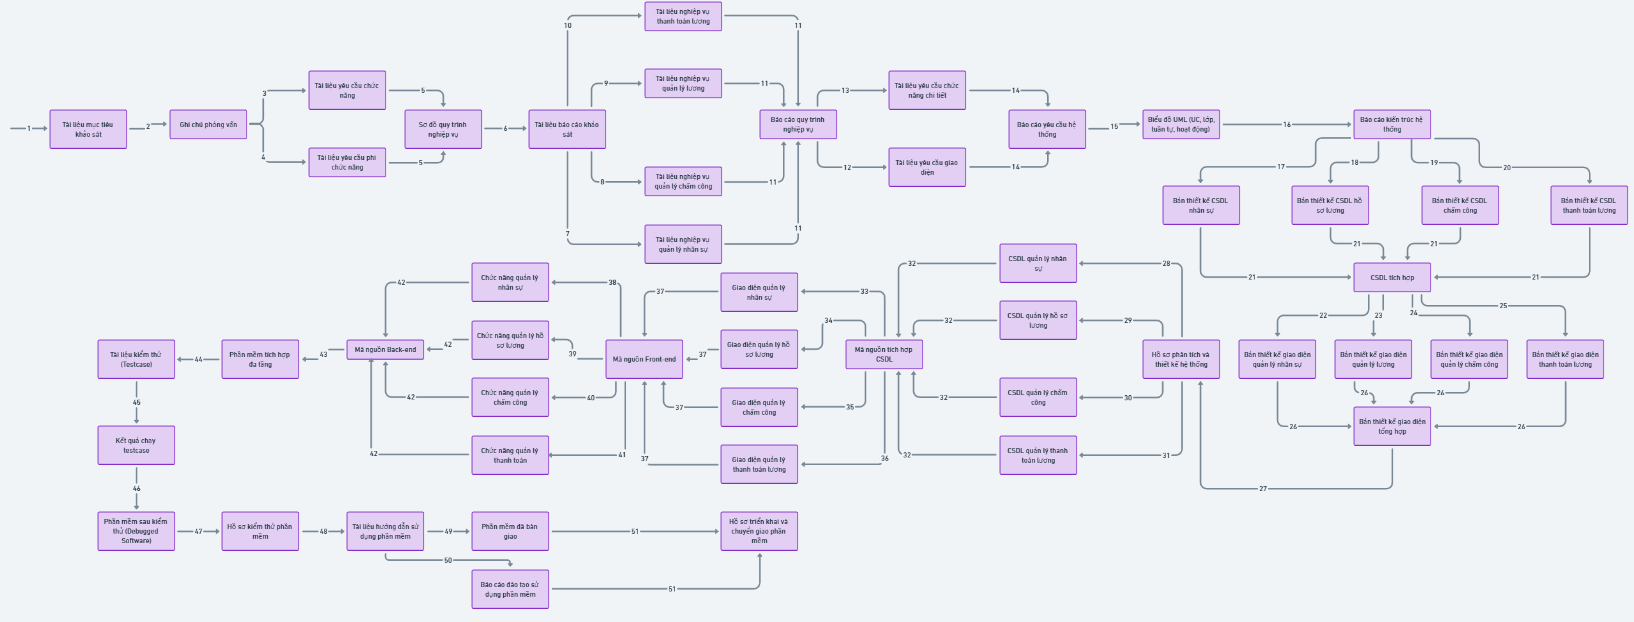
\includegraphics[width=\textwidth]{images/aoa.png}
    \caption{Sơ đồ AOA}
\end{figure}
\subsubsection{Sơ đồ AON}
\begin{figure}[H]
    \centering
    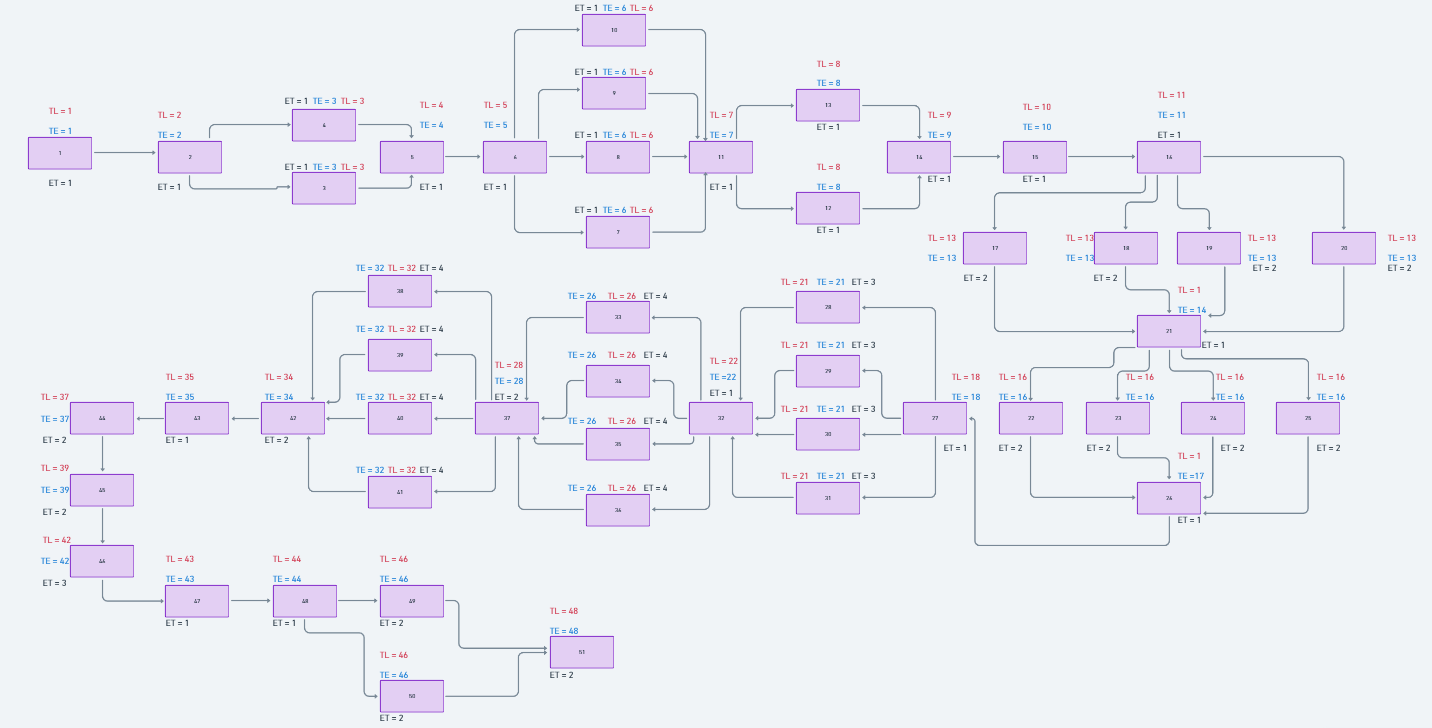
\includegraphics[width=\textwidth]{images/aon.png}
    \caption{Sơ đồ AON}
\end{figure}
\subsection{Sơ đồ Gantt}
\begin{figure}[H]
    \centering
    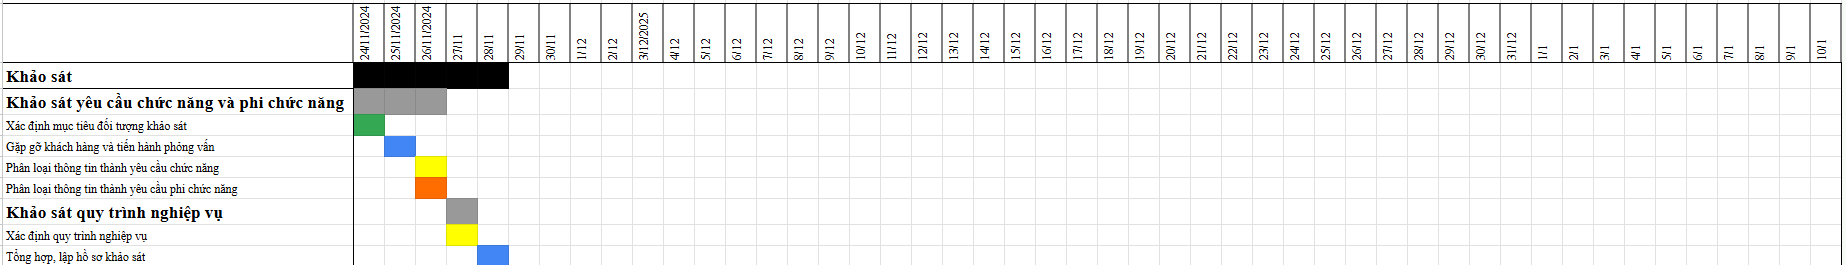
\includegraphics[width=\textwidth]{images/gantt1.png}
    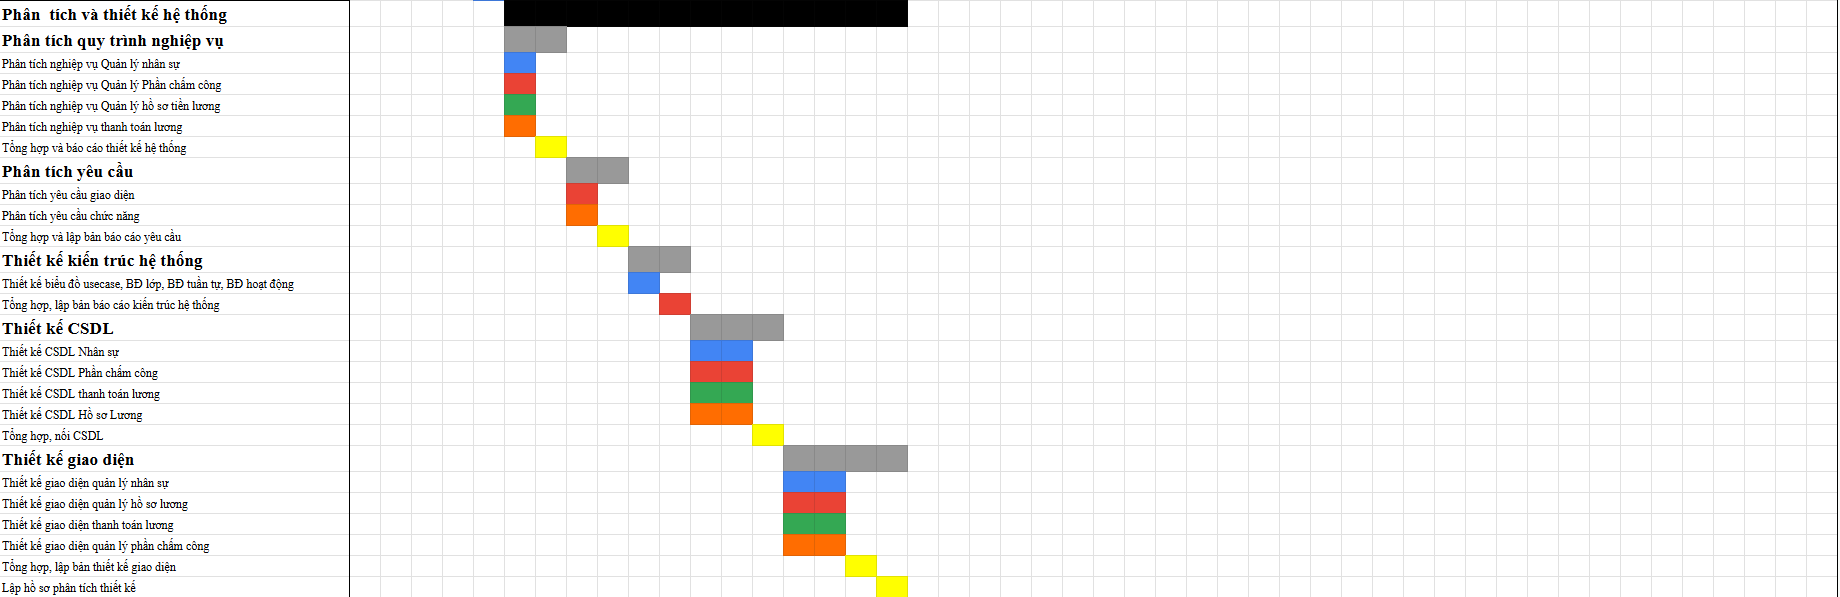
\includegraphics[width=\textwidth]{images/gantt2.png}
    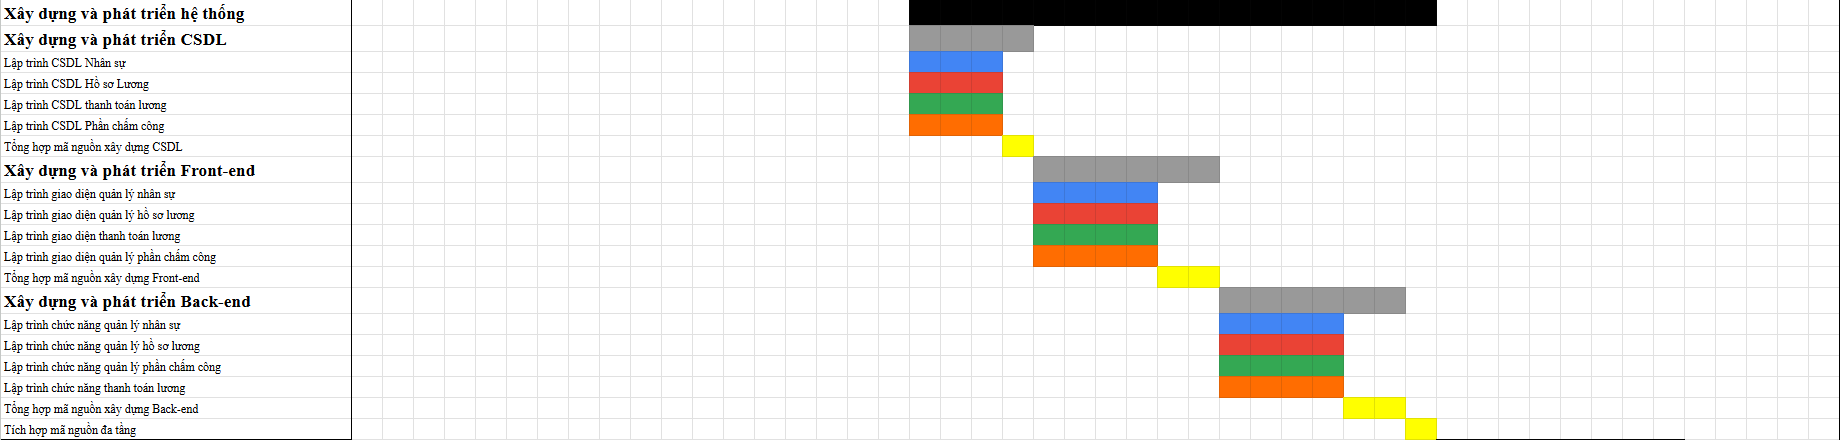
\includegraphics[width=\textwidth]{images/gantt3.png}
    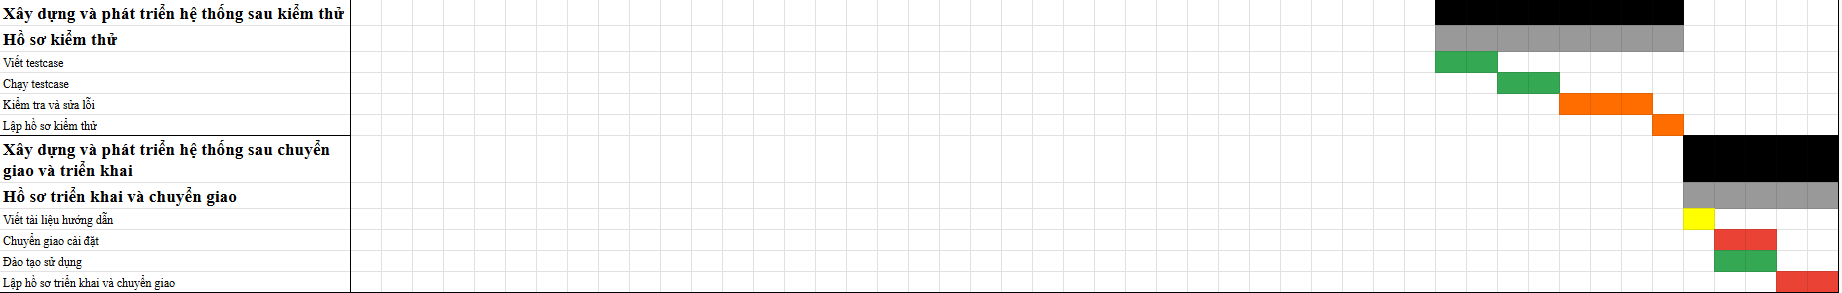
\includegraphics[width=\textwidth]{images/gantt4.png}
    \caption{Sơ đồ Gantt}
\end{figure}
\begin{figure}[H]
    \centering
    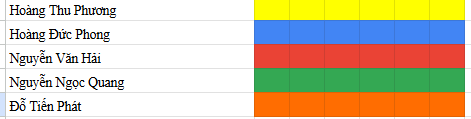
\includegraphics[width=\textwidth]{images/gantt_tv.png}
\end{figure}
\subsection{Tổng kết kế hoạch quản lý thời gian}
\clearpage
\begin{longtable}{|c|p{3cm}|c|c|c|p{2.8cm}|}
    \caption{Bảng phân chia công việc} \\ \hline
    \textbf{STT} & \textbf{Tên công việc} & \textbf{Thời gian (ngày)} & \textbf{Thời gian} & \textbf{Nhân lực} & \textbf{Sản phẩm} \\ \hline
    \endfirsthead
    \hline
    \textbf{STT} & \textbf{Tên công việc} & \textbf{Thời gian (ngày)} & \textbf{Thời gian} & \textbf{Nhân lực} & \textbf{Sản phẩm} \\ \hline
    \endhead
    \hline \multicolumn{6}{|r|}{{Tiếp theo trang sau}} \\ \hline
    \endfoot
    \hline
    \endlastfoot
    1 & Khảo sát & 5 & 24/11/2024 - 28/11/2024 & \hspace{0pt} & \hspace{0pt}\\ \hline
    1.1 & Khảo sát yêu cầu chức năng và phi chức năng & 3 & 24/11/2024 - 26/11/2024 & \hspace{0pt} & \hspace{0pt} \\ \hline
    1.1.1 & Xác định mục tiêu và đối tượng khảo sát & 1 & 24/11/2024 & Quang & Xác định được mục tiêu và đối tượng khảo sát \\ \hline
    1.1.2 & Gặp gỡ khách hàng và tiến hành phỏng vấn & 1 & 25/11/2024 & Phong & Thu thập được yêu cầu khách hàng \\ \hline
    1.1.3 & Phân loại thông tin thành yêu cầu chức năng & 1 & 26/11/2024 & Phương & Xác định được yêu cầu chức năng \\ \hline
    1.1.4 & Phân loại thông tin thành yêu cầu phi chức năng & 1 & 26/11/2024 & Phát & Xác định được yêu cầu phi chức năng \\ \hline
    1.2 & Khảo sát quy trình nghiệp vụ & 1 & 27/11/2024 & \hspace{0pt} & \hspace{0pt} \\ \hline
    1.2.1 & Xác định quy trình nghiệp vụ & 1 & 27/11/2024 & Phương & Xác định được quy trình nghiệp vụ \\ \hline
    1.3 & Tổng hợp, lập hồ sơ khảo sát & 1 & 28/11/2024 & Phong & Hồ sơ khảo sát \\ \hline
    2 & Phân tích và Thiết kế hệ thống & 13 & 29/11/2024 - 11/12/2024 & \hspace{0pt} & \hspace{0pt}\\ \hline
    2.1 & Phân tích quy trình nghiệp vụ & 2 & 29/11/2024 - 30/11/2024 & \hspace{0pt} & \hspace{0pt}\\ \hline
    2.1.1 & Phân tích nghiệp vụ Quản lý nhân sự & 1 & 29/11/2024 & Phong & Báo cáo nghiệp vụ quản lý nhân sự \\ \hline
    2.1.2 & Phân tích nghiệp vụ Quản lý Phần chấm công & 1 & 29/11/2024 & Quang & Báo cáo nghiệp vụ quản lý phần chấm công \\ \hline
    2.1.3 & Phân tích nghiệp vụ Quản lý hồ sơ tiền lương & 1 & 29/11/2024 & Hải & Báo cáo nghiệp vụ quản lý hồ sơ tiền lương \\ \hline
    2.1.4 & Phân tích nghiệp vụ thanh toán lương & 1 & 29/11/2024 & Phát & Báo cáo nghiệp vụ thanh toán lương \\ \hline
    2.1.5 & Tổng hợp và báo cáo thiết kế hệ thống & 1 & 30/11/2024 & Phương & Báo cáo thiết kế hệ thống \\ \hline
    2.2 & Phân tích yêu cầu & 2 & 1/12/2024 - 2/12/2024 & \hspace{0pt} & \hspace{0pt}\\ \hline
    2.2.1 & Phân tích yêu cầu giao diện & 1 & 1/12/2024 & Hải & Báo cáo yêu cầu giao diện \\ \hline
    2.2.2 & Phân tích yêu cầu chức năng & 1 & 1/12/2024 & Phát & Báo cáo yêu cầu chức năng \\ \hline
    2.2.3 & Tổng hợp và lập bản báo cáo yêu cầu & 1 & 2/12/2024 & Phương & Báo cáo yêu cầu \\ \hline
    2.3 & Thiết kế kiến trúc hệ thống & 2 & 3/12/2024 - 4/12/2024 & \hspace{0pt} & \hspace{0pt}\\ \hline
    2.3.1 & Thiết kế biểu đồ usecase, BĐ lớp, BĐ tuần tự, BĐ hoạt động & 1 & 3/12/2024 & Phong & Báo cáo các biểu đồ \\ \hline
    2.3.2 & Tổng hợp, lập bản báo cáo kiến trúc hệ thống & 1 & 4/12/2024 & Hải & Báo cáo kiến trúc hệ thống \\ \hline
    2.4 & Thiết kế CSDL & 3 & 5/12/2024 - 7/12/2024 & \hspace{0pt} & \hspace{0pt}\\ \hline
    2.4.1 & Thiết kế CSDL Nhân sự & 2 & 5/12/2024 - 6/12/2024 & Phong & Bản thiết kế CSDL nhân sự \\ \hline
    2.4.2 & Thiết kế CSDL Hồ sơ Lương & 2 & 5/12/2024 - 6/12/2024 & Hải & Bản thiết kế CSDL hồ sơ lương \\ \hline
    2.4.3 & Thiết kế CSDL Phần chấm công & 2 & 5/12/2024 - 6/12/2024 & Quang & Bản thiết kế CSDL phần chấm công \\ \hline
    2.4.4 & Thiết kế CSDL thanh toán lương & 2 & 5/12/2024 - 6/12/2024 & Phát & Bản thiết kế CSDL thanh toán lương \\ \hline
    2.4.5 & Tổng hợp, nối CSDL & 1 & 7/12/2024 & Phương & Bản thiết kế CSDL \\ \hline
    2.5 & Thiết kế giao diện & 4 & 8/12/2024 - 11/12/2024 & \hspace{0pt} & \hspace{0pt}\\ \hline
    2.5.1 & Thiết kế giao diện quản lý nhân sự & 2 & 8/12/2024 - 9/12/2024 & Phong & Bản thiết kế giao diện quản lý nhân sự \\ \hline
    2.5.2 & Thiết kế giao diện quản lý hồ sơ lương & 2 & 8/12/2024 - 9/12/2024 & Hải & Bản thiết kế giao diện quản lý hồ sơ lương \\ \hline
    2.5.3 & Thiết kế giao diện quản lý phần chấm công & 2 & 8/12/2024 - 9/12/2024 & Quang & Bản thiết kế giao diện quản lý phần chấm công \\ \hline
    2.5.4 & Thiết kế giao diện thanh toán lương & 2 & 8/12/2024 - 9/12/2024 & Phát & Bản thiết kế giao diện thanh toán lương \\ \hline
    2.5.5 & Tổng hợp, lập bản thiết kế giao diện & 1 & 10/12/2024 & Phương & Bản thiết kế giao diện \\ \hline
    2.6 & Lập hồ sơ phân tích thiết kế & 1 & 11/12/2024 & Phương & Hồ sơ phân tích thiết kế \\ \hline
    3 & Xây dựng và phát triển hệ thống & 17 & 12/12/2024 - 28/12/2024 & \hspace{0pt} & \hspace{0pt}\\ \hline
    3.1 & Xây dựng và phát triển CSDL & 4 & 12/12/2024 - 15/12/2024 & \hspace{0pt} & \hspace{0pt}\\ \hline
    3.1.1 & Lập trình CSDL Nhân sự & 3 & 12/12/2024 - 14/12/2024 & Phong & CSDL nhân sự \\ \hline
    3.1.2 & Lập trình CSDL Hồ sơ Lương & 3 & 12/12/2024 - 14/12/2024 & Hải & CSDL hồ sơ lương \\ \hline
    3.1.3 & Lập trình CSDL Phần chấm công & 3 & 12/12/2024 - 14/12/2024 & Quang & CSDL phần chấm công \\ \hline
    3.1.4 & Lập trình CSDL thanh toán lương & 3 & 12/12/2024 - 14/12/2024 & Phát & CSDL thanh toán lương \\ \hline
    3.1.5 & Tổng hợp mã nguồn xây dựng CSDL & 1 & 15/12/2024 & Phương & CSDL \\ \hline
    3.2 & Xây dựng và phát triển Front-end & 6 & 16/12/2024 - 21/12/2024 & \hspace{0pt} & \hspace{0pt}\\ \hline
    3.2.1 & Lập trình giao diện quản lý nhân sự & 4 & 16/12/2024 - 19/12/2024 & Phong & Giao diện quản lý nhân sự \\ \hline
    3.2.2 & Lập trình giao diện quản lý hồ sơ lương & 4 & 16/12/2024 - 19/12/2024 & Hải & Giao diện quản lý hồ sơ lương \\ \hline
    3.2.3 & Lập trình giao diện quản lý phần chấm công & 4 & 16/12/2024 - 19/12/2024 & Quang & Giao diện quản lý phần chấm công \\ \hline
    3.2.4 & Lập trình giao diện thanh toán lương & 4 & 16/12/2024 - 19/12/2024 & Phát & Giao diện thanh toán lương \\ \hline
    3.2.5 & Tổng hợp mã nguồn xây dựng Front-end & 2 & 20/12/2024 - 21/12/2024 & Phương & Giao diện \\ \hline
    3.3 & Xây dựng và phát triển Back-end & 7 & 22/12/2024 - 28/12/2024 & \hspace{0pt} & \hspace{0pt}\\ \hline
    3.3.1 & Lập trình chức năng quản lý nhân sự & 4 & 22/12/2024 - 25/12/2024 & Phong & Thực hiện được chức năng quản lý nhân sự \\ \hline
    3.3.2 & Lập trình chức năng quản lý hồ sơ lương & 4 & 22/12/2024 - 25/12/2024 & Hải & Thực hiện được chức năng quản lý hồ sơ lương \\ \hline
    3.3.3 & Lập trình chức năng quản lý phần chấm công & 4 & 22/12/2024 - 25/12/2024 & Quang & Thực hiện được chức năng quản lý phần chấm công \\ \hline
    3.3.4 & Lập trình chức năng thanh toán lương & 4 & 22/12/2024 - 25/12/2024 & Phát & Thực hiện được chức năng thanh toán lương \\ \hline
    3.3.5 & Tổng hợp mã nguồn xây dựng Back-end & 2 & 26/12/2024 - 27/12/2024 & Phương & Thực hiện được các chức năng \\ \hline
    3.4 & Tích hợp mã nguồn đa tầng & 1 & 28/12/2024 & Phương & Phần mềm \\ \hline
    4 & Xây dựng và phát triển phần mềm sau kiểm thử & 8 & 29/12/2024 - 5/1/2025 & \hspace{0pt} & \hspace{0pt}\\ \hline
    4.1 & Hồ sơ kiểm thử & 8 & 29/12/2024 - 5/1/2025 & \hspace{0pt} & \hspace{0pt}\\ \hline
    4.1.1 & Viết testcase & 2 & 29/12/2024 - 30/12/2024 & Quang & Viết testcase \\ \hline
    4.1.2 & Chạy testcase & 2 & 31/12/2024 - 1/1/2025 & Quang & Chạy testcase \\ \hline
    4.1.3 & Kiểm tra và sửa lỗi & 3 & 2/1/2025 - 4/1/2025 & Phát & Kiểm tra và sửa lỗi \\ \hline
    4.1.4 & Lập hồ sơ kiểm thử & 1 & 5/1/2025 & Phát & Phần mềm sau kiểm thử \\ \hline
    5 & Xây dựng và phát triển phần mềm sau triển khai và chuyển giao & 5 & 6/1/2025 - 10/1/2025 & \hspace{0pt} & \hspace{0pt}\\ \hline
    5.1 & Hồ sơ triển khai và chuyển giao & 5 & 6/1/2025 - 10/1/2025 & \hspace{0pt} & \hspace{0pt}\\ \hline
    5.1.1 & Viết tài liệu hướng dẫn & 1 & 6/1/2025 & Phương & Viết tài liệu hướng dẫn \\ \hline
    5.1.2 & Chuyển giao cài đặt & 2 & 7/1/2025 - 8/1/2025 & Hải & Chuyển giao cài đặt \\ \hline
    5.1.3 & Đào tạo sử dụng & 2 & 7/1/2025 - 8/1/2025 & Quang & Đào tạo sử dụng \\ \hline
    5.1.4 & Lập hồ sơ triển khai và chuyển giao & 2 & 9/1/2025 - 10/1/2025 & Hải & Phần mềm sau triển khai và bàn giao \\ \hline
\end{longtable}

\section{Kế hoạch quản lý chi phí}
\subsection{Kế hoạch cho nguồn tài nguyên}
\subsubsection{Tài sản cố định}
\begin{itemize}
    \item Các thiết bị phần cứng: máy chấm công.
\end{itemize}

\subsubsection{Chi phí vận hành}
\begin{itemize}
    \item Trả lương quản lý.
    \item Trả lương công việc.
\end{itemize}

\subsubsection{Chi phí phần mềm}
\begin{itemize}
    \item Domain, Hosting, Server
\end{itemize}

\subsubsection{Phúc lợi và hoạt động khác}
\begin{itemize}
    \item Liên hoan cuối tháng.
    \item Lương thưởng.
\end{itemize}

\subsection{Ước lượng chi phí}
\begin{table}[H]
    \caption{Ước lượng chi phí}
    \centering
    \renewcommand{\arraystretch}{1.5} % Tăng khoảng cách giữa các dòng
    \begin{tabular}{|c|c|}
        \hline
        \textbf{Đầu mục chi phí}                  & \textbf{Chi phí ước tính (VNĐ)} \\
        \hline
        Tài sản cố định                           & 44.400.000                      \\
        \hline
        Chi phí vận hành                          & 113.600.000                     \\
        \hline
        Chi phí phần mềm                          & 40.000.000                      \\
        \hline
        Phúc lợi và hoạt động khác                & 62.000.000                      \\
        \hline
        \multicolumn{1}{|c|}{\textbf{Tổng cộng:}} & \textbf{260.000.000}            \\
        \hline
    \end{tabular}
\end{table}

\subsection{Dự toán chi phí}
\subsubsection{Tài sản cố định}
\begin{table}[H]
    \caption{Dự toán chi phí tài sản cố định}
    \centering
    \renewcommand{\arraystretch}{1.5} % Tăng khoảng cách giữa các hàng
    \begin{tabular}{|c|c|c|c|c|}
        \hline
        \textbf{Hạng mục}                        & \textbf{Số lượng}   & \textbf{Đơn giá (VNĐ)} & \textbf{Đơn vị tính} & \textbf{Thành tiền (VNĐ)} \\
        \hline
        Máy chấm công                            & 1                   & 44.400.000             & Thiết bị             & 44.400.000                \\
        \hline
        \multicolumn{4}{|c|}{\textbf{Tổng cộng}} & \textbf{44.400.000}                                                                             \\
        \hline
    \end{tabular}
\end{table}


\subsubsection{Chi phí vận hành}
A. Trả lương quản lý
\begin{table}[H]
    \centering
    \renewcommand{\arraystretch}{1.5} % Tăng khoảng cách giữa các hàng
    \begin{tabular}{|p{3cm}|p{2.5cm}|p{2.3cm}|p{2cm}|p{3cm}|}
        \hline
        \textbf{Họ tên}                           & \textbf{Vị trí}     & \textbf{Mức lương (VND/Ngày)} & \textbf{Thời gian quản lý dự án (ngày)} & \textbf{Chi phí quản lý thực tế (VNĐ)} \\
        \hline
        Hoàng Thu Phương                          & Quản lý dự án       & 1.000.000                     & 48                                      & 48.000.000                             \\
        \hline
        \multicolumn{4}{|c|}{\textbf{Tổng cộng:}} & \textbf{48.000.000}                                                                                                                    \\
        \hline
    \end{tabular}
    \caption{Chi phí trả lương quản lý}
\end{table}

B. Trả lương công việc
\begin{table}[H]
    \centering
    \renewcommand{\arraystretch}{1.5} % Tăng khoảng cách giữa các hàng
    \caption{Bảng lương cơ bản theo vị trí}
    \begin{tabular}{|c|c|c|}
        \hline
        \textbf{Vị trí} & \textbf{Mức lương (VNĐ/Ngày)} & \textbf{Lương (VNĐ/Tháng)} \\
        \hline
        Quản lý dự án   & 1.000.000                     & 30.000.000                 \\
        \hline
        Nhân viên       & 600.000                       & 18.000.000                 \\
        \hline
    \end{tabular}
\end{table}

\clearpage
\begin{longtable}{|c|p{3cm}|c|c|c|c|p{3cm}|}
    \caption{WBS - Chi phí thực tế theo công việc}                                                                                                                                                                                                                                                         \\
    \hline
    \multirow{2}{*}{\textbf{WBS}}   & \multirow{2}{*}{\textbf{Tên công việc}}                       & \multicolumn{2}{c|}{\textbf{Thời gian (ngày)}} & \multicolumn{2}{c|}{\textbf{Số người tham gia}} & \multirow{2}{*}{\parbox{3cm}{\centering \textbf{Chi phí thực tế                                   \\ (VNĐ)}}} \\ \cline{3-6}
                                    &                                                               & \textbf{Kế hoạch}                              & \textbf{Thực tế}                                & \textbf{Quản lý}                                                & \textbf{Nhân viên} &            \\ \hline
    \endfirsthead
    \hline
    \multirow{2}{*}{\textbf{WBS}}   & \multirow{2}{*}{\textbf{Tên công việc}}                       & \multicolumn{2}{c|}{\textbf{Thời gian (ngày)}} & \multicolumn{2}{c|}{\textbf{Số người tham gia}} & \multirow{2}{*}{\parbox{3cm}{\centering \textbf{Chi phí thực tế                                   \\ (VNĐ)}}} \\ \cline{3-6}
                                    &                                                               & \textbf{Kế hoạch}                              & \textbf{Thực tế}                                & \textbf{Quản lý}                                                & \textbf{Nhân viên} &            \\ \hline
    \endhead
    \hline \multicolumn{7}{|r|}{{Tiếp theo trang sau}}                                                                                                                                                                                                                                                     \\ \hline
    \endfoot
    \hline
    \endlastfoot
    1                               & Khảo sát                                                      & 5                                              & 5                                               & 1                                                               & 3                  & 4.400.000  \\ \hline
    1.1                             & Khảo sát yêu cầu chức năng và phi chức năng                   & 3                                              & 3                                               & 1                                                               & 3                  & 2.800.000  \\ \hline
    1.1.1                           & Xác định mục tiêu và đối tượng khảo sát                       & 1                                              & 1                                               & 0                                                               & 1                  & 600.000    \\ \hline
    1.1.2                           & Gặp gỡ khách hàng và tiến hành phỏng vấn                      & 1                                              & 1                                               & 0                                                               & 1                  & 600.000    \\ \hline
    1.1.3                           & Phân loại thông tin thành yêu cầu chức năng                   & 1                                              & 1                                               & 1                                                               & 0                  & 1.000.000  \\ \hline
    1.1.4                           & Phân loại thông tin thành yêu cầu phi chức năng               & 1                                              & 1                                               & 0                                                               & 1                  & 600.000    \\ \hline
    1.2                             & Khảo sát quy trình nghiệp vụ                                  & 1                                              & 1                                               & 1                                                               & 0                  & 1.000.000  \\ \hline
    1.2.1                           & Xác định quy trình nghiệp vụ                                  & 1                                              & 1                                               & 1                                                               & 0                  & 1.000.000  \\ \hline
    1.3                             & Tổng hợp, lập hồ sơ khảo sát                                  & 1                                              & 1                                               & 0                                                               & 1                  & 600.000    \\ \hline
    2                               & Phân tích và Thiết kế hệ thống                                & 13                                             & 13                                              & 1                                                               & 4                  & 19.400.000 \\ \hline
    2.1                             & Phân tích quy trình nghiệp vụ                                 & 2                                              & 2                                               & 1                                                               & 4                  & 3.400.000  \\ \hline
    2.1.1                           & Phân tích nghiệp vụ Quản lý nhân sự                           & 1                                              & 1                                               & 0                                                               & 1                  & 600.000    \\ \hline
    2.1.2                           & Phân tích nghiệp vụ Quản lý Phần chấm công                    & 1                                              & 1                                               & 0                                                               & 1                  & 600.000    \\ \hline
    2.1.3                           & Phân tích nghiệp vụ Quản lý hồ sơ tiền lương                  & 1                                              & 1                                               & 0                                                               & 1                  & 600.000    \\ \hline
    2.1.4                           & Phân tích nghiệp vụ thanh toán lương                          & 1                                              & 1                                               & 0                                                               & 1                  & 600.000    \\ \hline
    2.1.5                           & Tổng hợp và báo cáo thiết kế hệ thống                         & 1                                              & 1                                               & 1                                                               & 0                  & 1.000.000  \\ \hline
    2.2                             & Phân tích yêu cầu                                             & 2                                              & 2                                               & 1                                                               & 2                  & 2.200.000  \\ \hline
    2.2.1                           & Phân tích yêu cầu giao diện                                   & 1                                              & 1                                               & 0                                                               & 1                  & 600.000    \\ \hline
    2.2.2                           & Phân tích yêu cầu chức năng                                   & 1                                              & 1                                               & 0                                                               & 1                  & 600.000    \\ \hline
    2.2.3                           & Tổng hợp và lập bản báo cáo yêu cầu                           & 1                                              & 1                                               & 1                                                               & 0                  & 1.000.000  \\ \hline
    2.3                             & Thiết kế kiến trúc hệ thống                                   & 2                                              & 2                                               & 0                                                               & 2                  & 1.200.000  \\ \hline
    2.3.1                           & Thiết kế biểu đồ usecase, BĐ lớp, BĐ tuần tự, BĐ hoạt động    & 1                                              & 1                                               & 0                                                               & 1                  & 600.000    \\ \hline
    2.3.2                           & Tổng hợp, lập bản báo cáo kiến trúc hệ thống                  & 1                                              & 1                                               & 0                                                               & 1                  & 600.000    \\ \hline
    2.4                             & Thiết kế CSDL                                                 & 3                                              & 3                                               & 1                                                               & 4                  & 5.800.000  \\ \hline
    2.4.1                           & Thiết kế CSDL Nhân sự                                         & 2                                              & 2                                               & 0                                                               & 1                  & 1.200.000  \\ \hline
    2.4.2                           & Thiết kế CSDL Hồ sơ Lương                                     & 2                                              & 2                                               & 0                                                               & 1                  & 1.200.000  \\ \hline
    2.4.3                           & Thiết kế CSDL Phần chấm công                                  & 2                                              & 2                                               & 0                                                               & 1                  & 1.200.000  \\ \hline
    2.4.4                           & Thiết kế CSDL thanh toán lương                                & 2                                              & 2                                               & 0                                                               & 1                  & 1.200.000  \\ \hline
    2.4.5                           & Tổng hợp, nối CSDL                                            & 1                                              & 1                                               & 1                                                               & 0                  & 1.000.000  \\ \hline
    2.5                             & Thiết kế giao diện                                            & 4                                              & 4                                               & 1                                                               & 4                  & 5.800.000  \\ \hline
    2.5.1                           & Thiết kế giao diện quản lý nhân sự                            & 2                                              & 2                                               & 0                                                               & 1                  & 1.200.000  \\ \hline
    2.5.2                           & Thiết kế giao diện quản lý hồ sơ lương                        & 2                                              & 2                                               & 0                                                               & 1                  & 1.200.000  \\ \hline
    2.5.3                           & Thiết kế giao diện quản lý phần chấm công                     & 2                                              & 2                                               & 0                                                               & 1                  & 1.200.000  \\ \hline
    2.5.4                           & Thiết kế giao diện thanh toán lương                           & 2                                              & 2                                               & 0                                                               & 1                  & 1.200.000  \\ \hline
    2.5.5                           & Tổng hợp, lập bản thiết kế giao diện                          & 1                                              & 1                                               & 1                                                               & 0                  & 1.000.000  \\ \hline
    2.6                             & Lập hồ sơ phân tích thiết kế                                  & 1                                              & 1                                               & 1                                                               & 0                  & 1.000.000  \\ \hline
    3                               & Xây dựng và phát triển hệ thống                               & 17                                             & 17                                              & 1                                                               & 4                  & 32.400.000 \\ \hline
    3.1                             & Xây dựng và phát triển CSDL                                   & 4                                              & 4                                               & 1                                                               & 4                  & 8.200.000  \\ \hline
    3.1.1                           & Lập trình CSDL Nhân sự                                        & 3                                              & 3                                               & 0                                                               & 1                  & 1.800.000  \\ \hline
    3.1.2                           & Lập trình CSDL Hồ sơ Lương                                    & 3                                              & 3                                               & 0                                                               & 1                  & 1.800.000  \\ \hline
    3.1.3                           & Lập trình CSDL Phần chấm công                                 & 3                                              & 3                                               & 0                                                               & 1                  & 1.800.000  \\ \hline
    3.1.4                           & Lập trình CSDL thanh toán lương                               & 3                                              & 3                                               & 0                                                               & 1                  & 1.800.000  \\ \hline
    3.1.5                           & Tổng hợp mã nguồn xây dựng CSDL                               & 1                                              & 1                                               & 1                                                               & 0                  & 1.000.000  \\ \hline
    3.2                             & Xây dựng và phát triển Front-end                              & 6                                              & 6                                               & 1                                                               & 4                  & 11.600.000 \\ \hline
    3.2.1                           & Lập trình giao diện quản lý nhân sự                           & 4                                              & 4                                               & 0                                                               & 1                  & 2.400.000  \\ \hline
    3.2.2                           & Lập trình giao diện quản lý hồ sơ lương                       & 4                                              & 4                                               & 0                                                               & 1                  & 2.400.000  \\ \hline
    3.2.3                           & Lập trình giao diện quản lý phần chấm công                    & 4                                              & 4                                               & 0                                                               & 1                  & 2.400.000  \\ \hline
    3.2.4                           & Lập trình giao diện thanh toán lương                          & 4                                              & 4                                               & 0                                                               & 1                  & 2.400.000  \\ \hline
    3.2.5                           & Tổng hợp mã nguồn xây dựng Front-end                          & 2                                              & 2                                               & 1                                                               & 0                  & 2.000.000  \\ \hline
    3.3                             & Xây dựng và phát triển Back-end                               & 7                                              & 7                                               & 1                                                               & 4                  & 11.600.000 \\ \hline
    3.3.1                           & Lập trình chức năng quản lý nhân sự                           & 4                                              & 4                                               & 0                                                               & 1                  & 2.400.000  \\ \hline
    3.3.2                           & Lập trình chức năng quản lý hồ sơ lương                       & 4                                              & 4                                               & 0                                                               & 1                  & 2.400.000  \\ \hline
    3.3.3                           & Lập trình chức năng quản lý phần chấm công                    & 4                                              & 4                                               & 0                                                               & 1                  & 2.400.000  \\ \hline
    3.3.4                           & Lập trình chức năng thanh toán lương                          & 4                                              & 4                                               & 0                                                               & 1                  & 2.400.000  \\ \hline
    3.3.5                           & Tổng hợp mã nguồn xây dựng Back-end                           & 2                                              & 2                                               & 1                                                               & 0                  & 2.000.000  \\ \hline
    3.4                             & Tích hợp mã nguồn đa tầng                                     & 1                                              & 1                                               & 1                                                               & 0                  & 1.000.000  \\ \hline
    4                               & Xây dựng và phát triển phần mềm sau kiểm thử                  & 8                                              & 8                                               & 0                                                               & 2                  & 4.800.000  \\ \hline
    4.1                             & Hồ sơ kiểm thử                                                & 8                                              & 8                                               & 0                                                               & 2                  & 4.800.000  \\ \hline
    4.1.1                           & Viết testcase                                                 & 2                                              & 2                                               & 0                                                               & 1                  & 1.200.000  \\ \hline
    4.1.2                           & Chạy testcase                                                 & 2                                              & 2                                               & 0                                                               & 1                  & 1.200.000  \\ \hline
    4.1.3                           & Kiểm tra và sửa lỗi                                           & 3                                              & 3                                               & 0                                                               & 1                  & 1.800.000  \\ \hline
    4.1.4                           & Lập hồ sơ kiểm thử                                            & 1                                              & 1                                               & 0                                                               & 1                  & 600.000    \\ \hline
    5                               & Xây dựng và phát triển phần mềm sau triển khai và chuyển giao & 5                                              & 5                                               & 1                                                               & 2                  & 4.600.000  \\ \hline
    5.1                             & Hồ sơ triển khai và chuyển giao                               & 5                                              & 5                                               & 1                                                               & 2                  & 4.600.000  \\ \hline
    5.1.1                           & Viết tài liệu hướng dẫn                                       & 1                                              & 1                                               & 1                                                               & 0                  & 1.000.000  \\ \hline
    5.1.2                           & Chuyển giao cài đặt                                           & 2                                              & 2                                               & 0                                                               & 1                  & 1.200.000  \\ \hline
    5.1.3                           & Đào tạo sử dụng                                               & 2                                              & 2                                               & 0                                                               & 1                  & 1.200.000  \\ \hline
    5.1.4                           & Lập hồ sơ triển khai và chuyển giao                           & 2                                              & 2                                               & 0                                                               & 1                  & 1.200.000  \\ \hline
    \multicolumn{6}{|c|}{Tổng cộng} & 65.600.000                                                                                                                                                                                                                                                           \\ \hline
\end{longtable}

\begin{tabbing}
    Tổng CPVH (*): 65.600.000 + 48.000.000 = \= 113.600.000 (VNĐ) \\
    *: Chi phí vận hành gồm: Chi phí quản lý và chi phí thực tế theo phân chia công việc \\
    ( được trình bày ở phần B.Trả lương công việc ) %  % Dòng này sẽ xuống dòng nhưng vẫn thẳng hàng
\end{tabbing}

\subsubsection{Chi phí phần mềm}
\begin{table}[H]
    \centering
    \renewcommand{\arraystretch}{1.5} % Tăng khoảng cách giữa các hàng
    \caption{Dự toán chi phí phần mềm}
    \begin{tabular}{|c|c|c|c|c|}
        \hline
        \textbf{Hạng mục}                         & \textbf{Số lượng}   & \textbf{Đơn giá (VNĐ)} & \textbf{Đơn vị tính} & \textbf{Thành tiền (VNĐ)} \\
        \hline
        Domain                                    & 1                   & 500.000                & Năm                  & 500.000                   \\
        \hline
        Hosting                                   & 1                   & 1.500.000              & Năm                  & 1.500.000                 \\
        \hline
        Server                                    & 1                   & 38.000.000             & Năm                  & 38.000.000                \\
        \hline
        \multicolumn{4}{|c|}{\textbf{Tổng cộng:}} & \textbf{40.000.000}                                                                             \\
        \hline
    \end{tabular}
\end{table}


\subsubsection{Phúc lợi và hoạt động khác}
\begin{table}[H]
    \centering
    \renewcommand{\arraystretch}{1.5} % Tăng khoảng cách giữa các hàng
    \caption{Dự toán chi phí phúc lợi và hoạt động khác}
    \begin{tabular}{|c|c|c|c|c|}
        \hline
        \textbf{Hạng mục}                         & \textbf{Số lượng}   & \textbf{Đơn giá (VNĐ)} & \textbf{Đơn vị tính} & \textbf{Thành tiền (VNĐ)} \\
        \hline
        Liên hoan cuối tháng                      & 2                   & 6.000.000              & Tháng                & 12.000.000                \\
        \hline
        Lương thưởng                              & 1                   & 50.000.000             & Lần                  & 50.000.000                \\
        \hline
        \multicolumn{4}{|c|}{\textbf{Tổng cộng:}} & \textbf{62.000.000}                                                                             \\
        \hline
    \end{tabular}
\end{table}

\subsection{Quản lý chi phí chia theo giai đoạn dự án}
\subsubsection{Bảng phân bổ chi phí theo giai đoạn dự án}
\begin{table}[H]
    \centering
    \renewcommand{\arraystretch}{1.5} % Tăng khoảng cách giữa các hàng
    \caption{Bảng phân bổ chi phí theo giai đoạn dự án}
    \begin{tabular}{|c|c|}
        \hline
        \textbf{Giai đoạn}                        & \textbf{Chi phí (VNĐ)} \\
        \hline
        Khảo sát                                  & 9.400.000              \\
        \hline
        Phân tích và Thiết kế                     & 76.800.000             \\
        \hline
        Xây dựng và phát triển                    & 89.400.000             \\
        \hline
        Kiểm thử                                  & 18.800.000             \\
        \hline
        Triển khai và bàn giao                    & 65.600.000             \\
        \hline
        \multicolumn{1}{|c|}{\textbf{Tổng cộng:}} & \textbf{260.000.000}   \\
        \hline
    \end{tabular}
\end{table}


\subsubsection{Quản lý chi phí chi tiết theo giai đoạn dự án}
Giai đoạn 1: Khảo sát
\begin{tabbing}
    Thời gian: \= 5 ngày. \\
    Chi phí chi tiết: %  % Dòng này sẽ xuống dòng nhưng vẫn thẳng hàng
\end{tabbing}
\begin{itemize}
    \item Chi phí nhân sự: 4.400.000 VNĐ.
    \item Chi phí quản lý: 5.000.000 VNĐ.
    \item Tổng chi phí: 9.400.000 VNĐ.
\end{itemize}

Giai đoạn 2: Phân tích và Thiết kế
\begin{tabbing}
    Thời gian: \= 13 ngày. \\
    Chi phí chi tiết: %  % Dòng này sẽ xuống dòng nhưng vẫn thẳng hàng
\end{tabbing}
\begin{itemize}
    \item Chi phí nhân sự: 19.400.000 VNĐ.
    \item Chi phí quản lý: 13.000.000 VNĐ.
    \item Chi phí mua thiết bị phần cứng (Máy chấm công): 44.400.000 VNĐ.
    \item Tổng chi phí: 76.800.000 VNĐ.
\end{itemize}

Giai đoạn 3: Xây dựng và phát triển
\begin{tabbing}
    Thời gian: \= 17 ngày. \\
    Chi phí chi tiết: %  % Dòng này sẽ xuống dòng nhưng vẫn thẳng hàng
\end{tabbing}
\begin{itemize}
    \item Chi phí nhân sự: 32.400.000 VNĐ.
    \item Chi phí quản lý: 17.000.000 VNĐ.
    \item Chi phí phần mềm (Hosting, Server, Domain): 40.000.000 VNĐ.
    \item Tổng chi phí: 89.400.000 VNĐ.
\end{itemize}

Giai đoạn 4: Kiểm thử
\begin{tabbing}
    Thời gian: \= 8 ngày. \\
    Chi phí chi tiết: %  % Dòng này sẽ xuống dòng nhưng vẫn thẳng hàng
\end{tabbing}
\begin{itemize}
    \item Chi phí nhân sự: 4.800.000 VNĐ.
    \item Chi phí quản lý: 8.000.000 VNĐ.
    \item Chi phí liên hoan: 6.000.000 VNĐ.
    \item Tổng chi phí: 18.800.000 VNĐ.
\end{itemize}

Giai đoạn 5: Triển khai và bàn giao
\begin{tabbing}
    Thời gian: \= 5 ngày. \\
    Chi phí chi tiết: %  % Dòng này sẽ xuống dòng nhưng vẫn thẳng hàng
\end{tabbing}
\begin{itemize}
    \item Chi phí nhân sự: 4.600.000 VNĐ.
    \item Chi phí quản lý: 5.000.000 VNĐ.
    \item Chi phí phúc lợi và hoạt động khác (Liên hoan, lương thưởng): 56.000.000 VNĐ.
    \item Tổng chi phí: 65.600.000 VNĐ.
\end{itemize}

\subsubsection{Tổng chi phí dự án}
\begin{itemize}
    \item Tổng chi phí nhân sự: 65.600.000 VNĐ
    \item Tổng chi phí quản lý: 48.000.000 VNĐ
    \item Tổng chi phí mua thiết bị: 44.400.000 VNĐ
    \item Tổng chi phí phần mềm: 40.000.000 VNĐ
    \item Tổng chi phí phúc lợi và hoạt động khác: 62.000.000 VNĐ
\end{itemize}
\textbf{Tổng chi phí dự án: 260.000.000 VNĐ}
